\documentclass[11pt]{article}

\usepackage{tocloft}
\usepackage[margin=1in]{geometry} %used for margins
\usepackage{graphics}
\usepackage{graphicx}
\usepackage{gensymb} %for symbols such as the degree sign
% \usepackage{fixltx2e}
\usepackage{titlesec}
\graphicspath{
{../../figures/stimuli/experiment1/before/}
{../../figures/stimuli/experiment1/after/}
{../../figures/stimuli/experiment2/}
{../../figures/stimuli/experiment2/initial/}
{../../figures/stimuli/experiment2/final/}
{../../figures/stimuli/experiment3/initial_labeled/}
{../../figures/stimuli/experiment4/initial_small/}
{../../figures/plots/selected_bricks/}
{../../figures/plots/}
{../../figures/plots/selected_bricks/}
{../../figures/screenshots/}
}
\usepackage[natbibapa]{apacite}
\usepackage{xcolor}
\usepackage{array}% http://ctan.org/pkg/array
\usepackage{tikz} %used for drawing colored boxes 
\usepackage{bibentry} %for full citations
% \nobibliography* 
\usepackage{subfig} %for creating panels
% \usepackage{subcaption} %for creating panels
\usepackage{todonotes}  
\usepackage{booktabs}% http://ctan.org/pkg/booktabs
\usepackage{ctable}% http://ctan.org/pkg/booktabs
\usepackage[countmax]{subfloat} %for creating panels
\usepackage{enumitem} %better environment for lists 
\usepackage{multirow} %to have multiple row entries in tables 
\usepackage{breakurl} %to break urls
\usepackage{wrapfig} %to wrap figures
\usepackage{float}  %for floating figures
\usepackage{amsmath}
\usepackage{hyperref} %to h ave links within the document 
\hypersetup{
    colorlinks,%
    citecolor=black,%
    filecolor=black,%
    linkcolor=black,%
    urlcolor=black
}

%to allow for more figures per page 
\renewcommand\floatpagefraction{.95}
\renewcommand\topfraction{.95}
\renewcommand\bottomfraction{.95}
\renewcommand\textfraction{.05}   
\setcounter{totalnumber}{200}
\setcounter{topnumber}{200}
\setcounter{bottomnumber}{200}

%some settings to make lists look nicer 
\setlist{leftmargin=*} 
\setlist[1]{labelindent=\parindent} % Only the level 1
\setlist{topsep = 0cm,partopsep = 1pt, parsep = 1pt} %changes the separation of lists 

%some stuff to decrease the space around section headings, etc. 
\titleformat{\section}
  {\bfseries \Large}{\thesection}{0.5em}{}

\titleformat{\subsection}
  {\bfseries \large}{\thesubsection}{0.5em}{}

\titleformat{\subsubsection}
{\bfseries}{\thesubsubsection}{0.5em}{}

\titlespacing{\section}{0cm}{0.3cm}{0.1cm}
\titlespacing{\subsection}{0cm}{0.3cm}{0.1cm}
\titlespacing{\subsubsection}{0cm}{0.3cm}{0.1cm}

%special trick for having vertically aligned table entries (just use M instead of the normal ways of defining table columns)
\newcolumntype{M}{>{\centering\arraybackslash}m{\dimexpr.2\linewidth-2\tabcolsep}}

%command to create boxes 
\newcommand{\mycbox}[2]{\tikz{\path[draw=#1,fill=#2] (0,0) rectangle (1cm,1cm);}}

%nice to do notes
\newcommand{\ttodo}[2][]
{\todo[caption={#2}, size=\small, #1]{\renewcommand{\baselinestretch}{1}\selectfont#2\par}~}

%for tick marks
\usepackage{pifont}% http://ctan.org/pkg/pifont
\newcommand{\cmark}{\ding{51}}%
\newcommand{\xmark}{\ding{55}}%

%for possessive citing
\def\citeapos#1{\citeauthor{#1}'s (\citeyear{#1})}

\begin{document}

\begin{center} 
{\LARGE \textbf{Faulty Towers}}
\linebreak
\linebreak
{\large Tobias Gerstenberg (\href{mailto:tger@mit.edu}{tger@mit.edu}),
 Liang Zhou, Kevin Smith, Josh Tenenbaum}
\linebreak
\today
\end{center} 

\tableofcontents 
\clearpage

% \section{Experiment 1}
% \label{sec:experiment_1}

% \subsection{Methods}
% \label{sub:methods}

% \begin{figure}[H]
% \centering
% {\hfill}
% \subfloat[][Instructions]{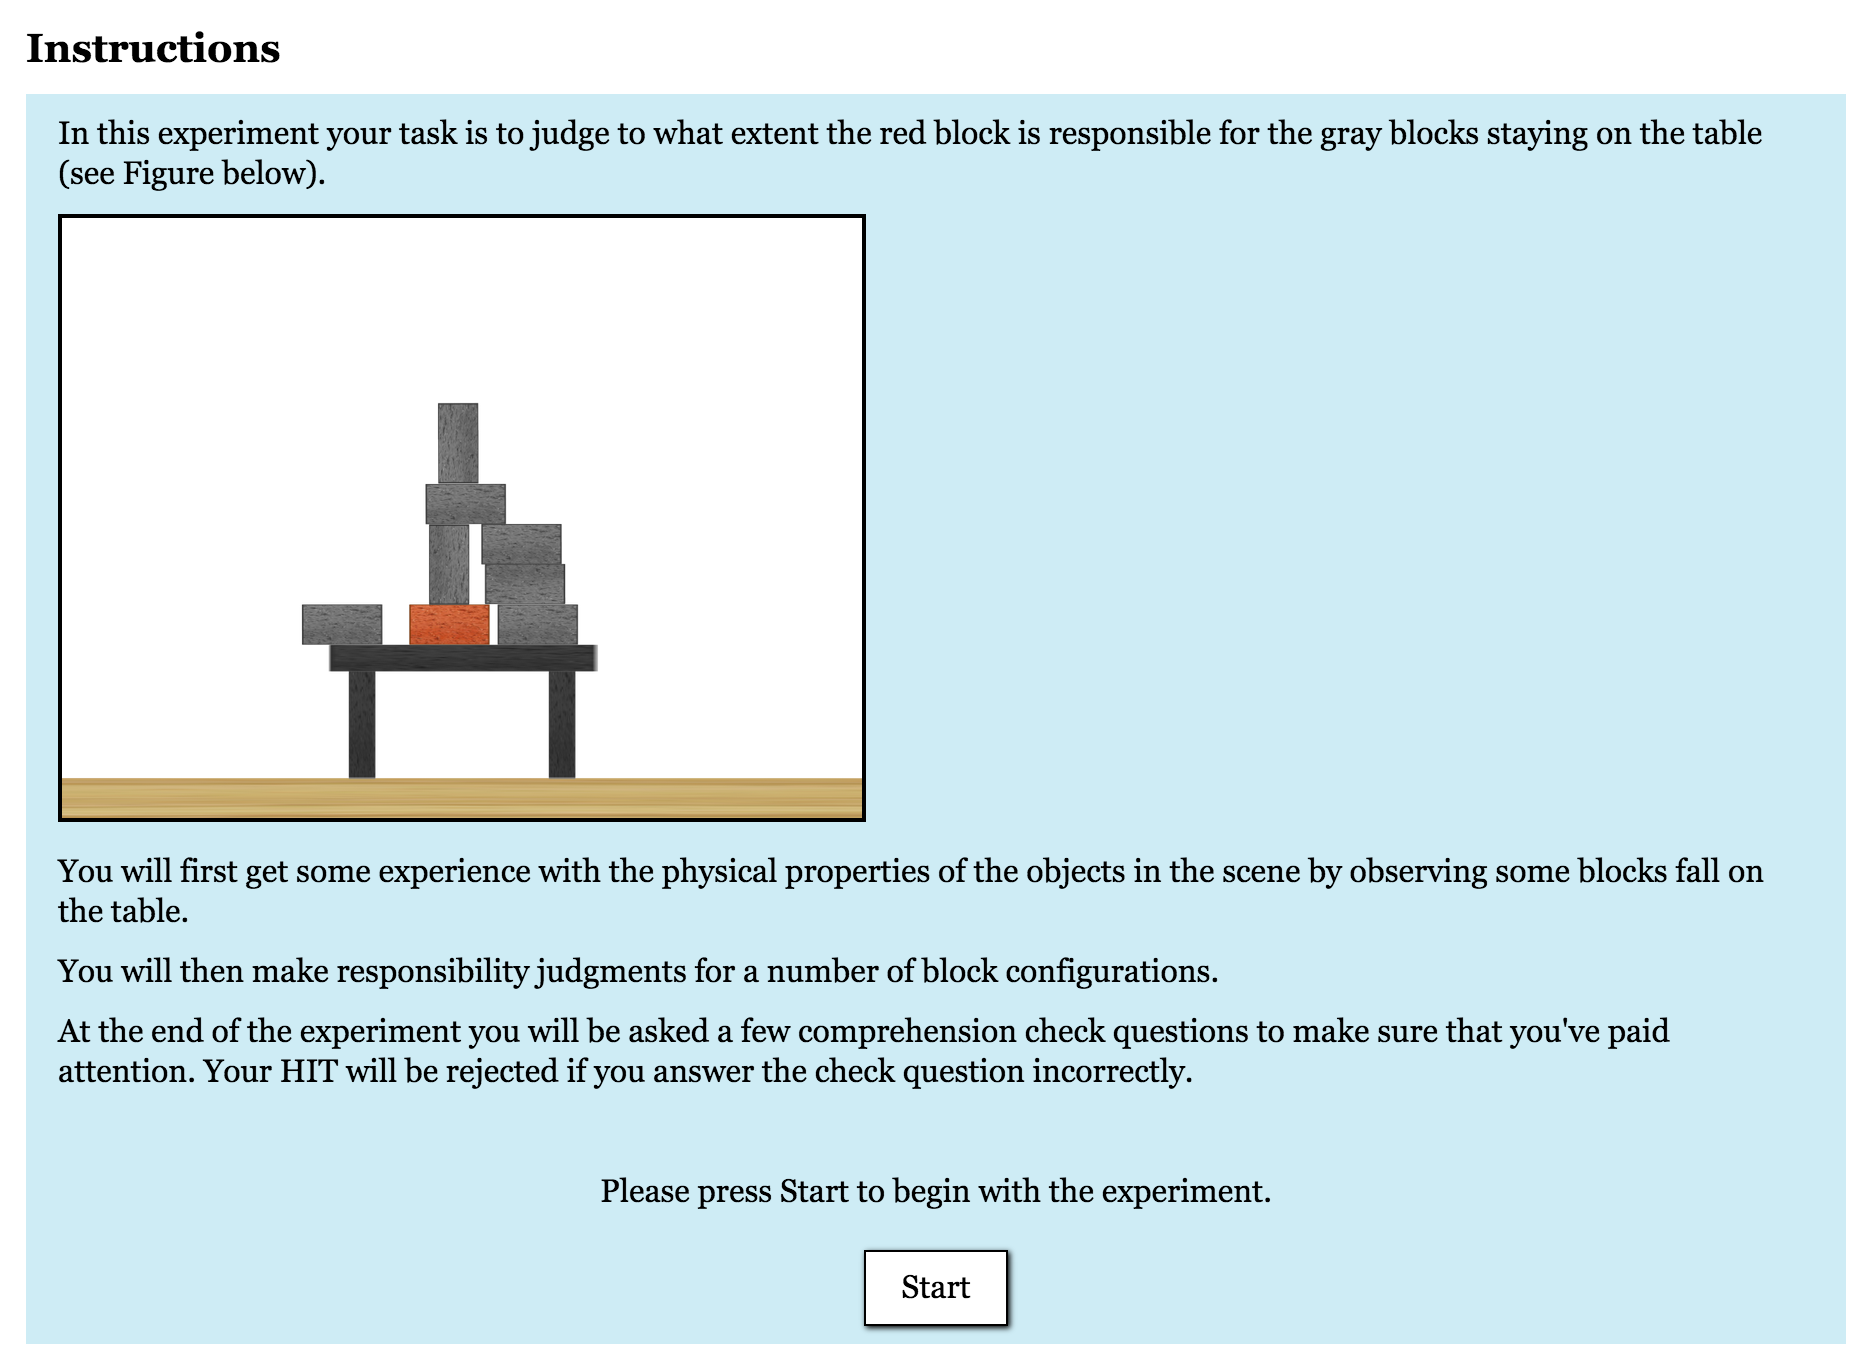
\includegraphics[width=0.32\columnwidth]{exp1_screenshot_1}}
% \hfill
% \subfloat[][Observations]{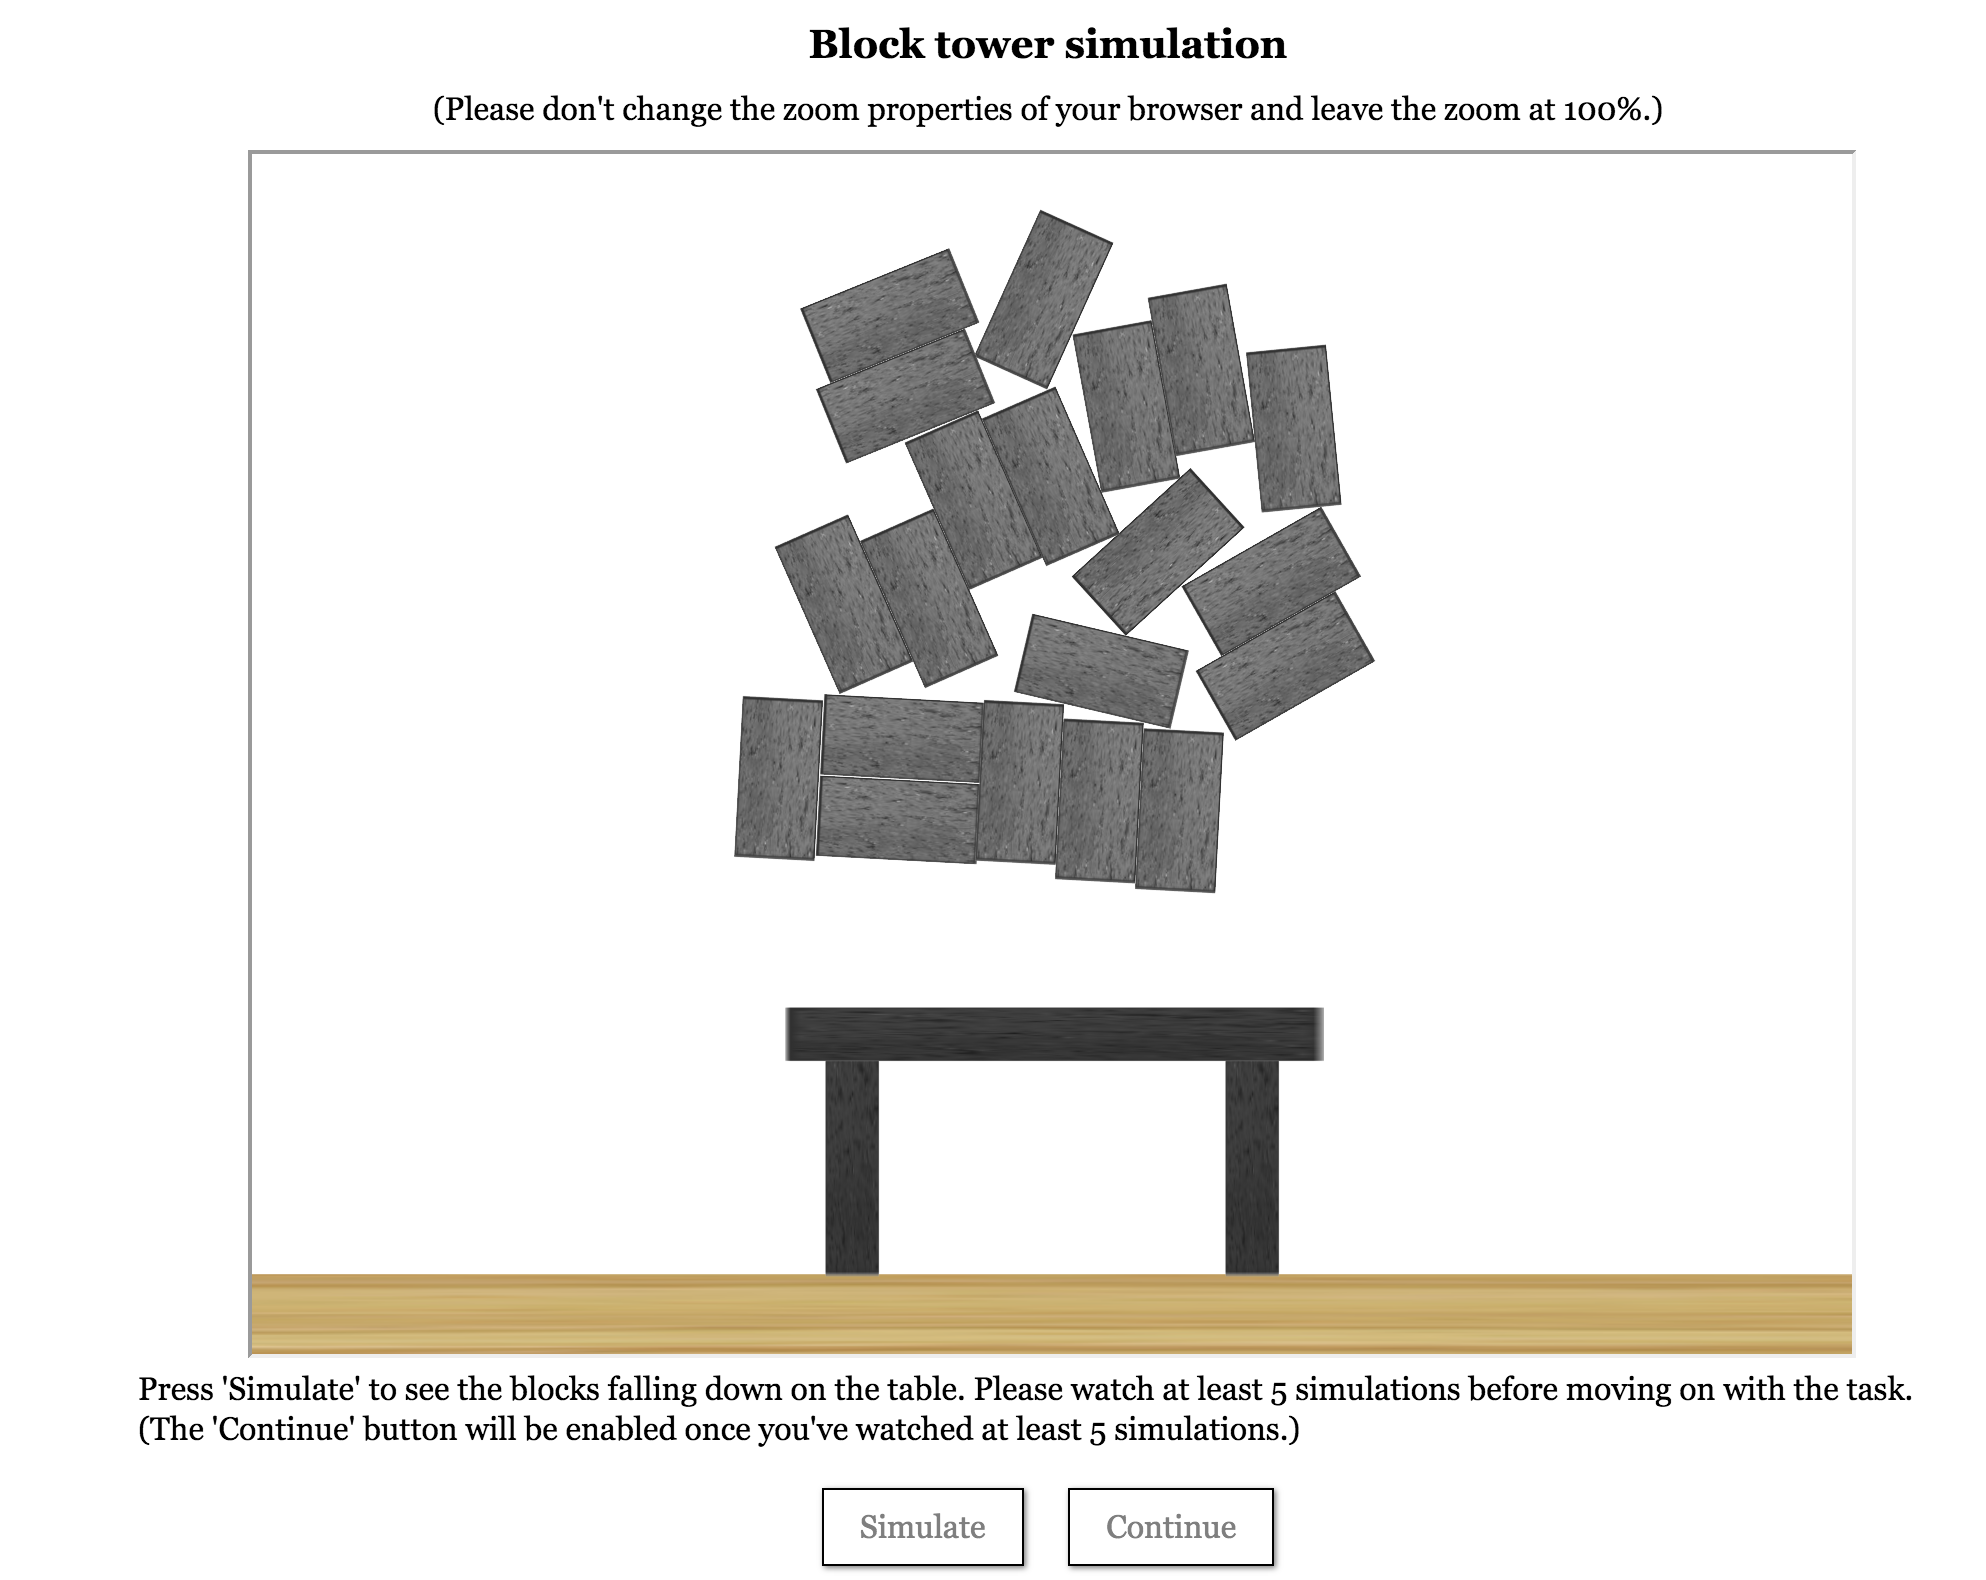
\includegraphics[width=0.32\columnwidth]{exp1_screenshot_2}}
% \hfill
% \subfloat[][Responsibility judgments]{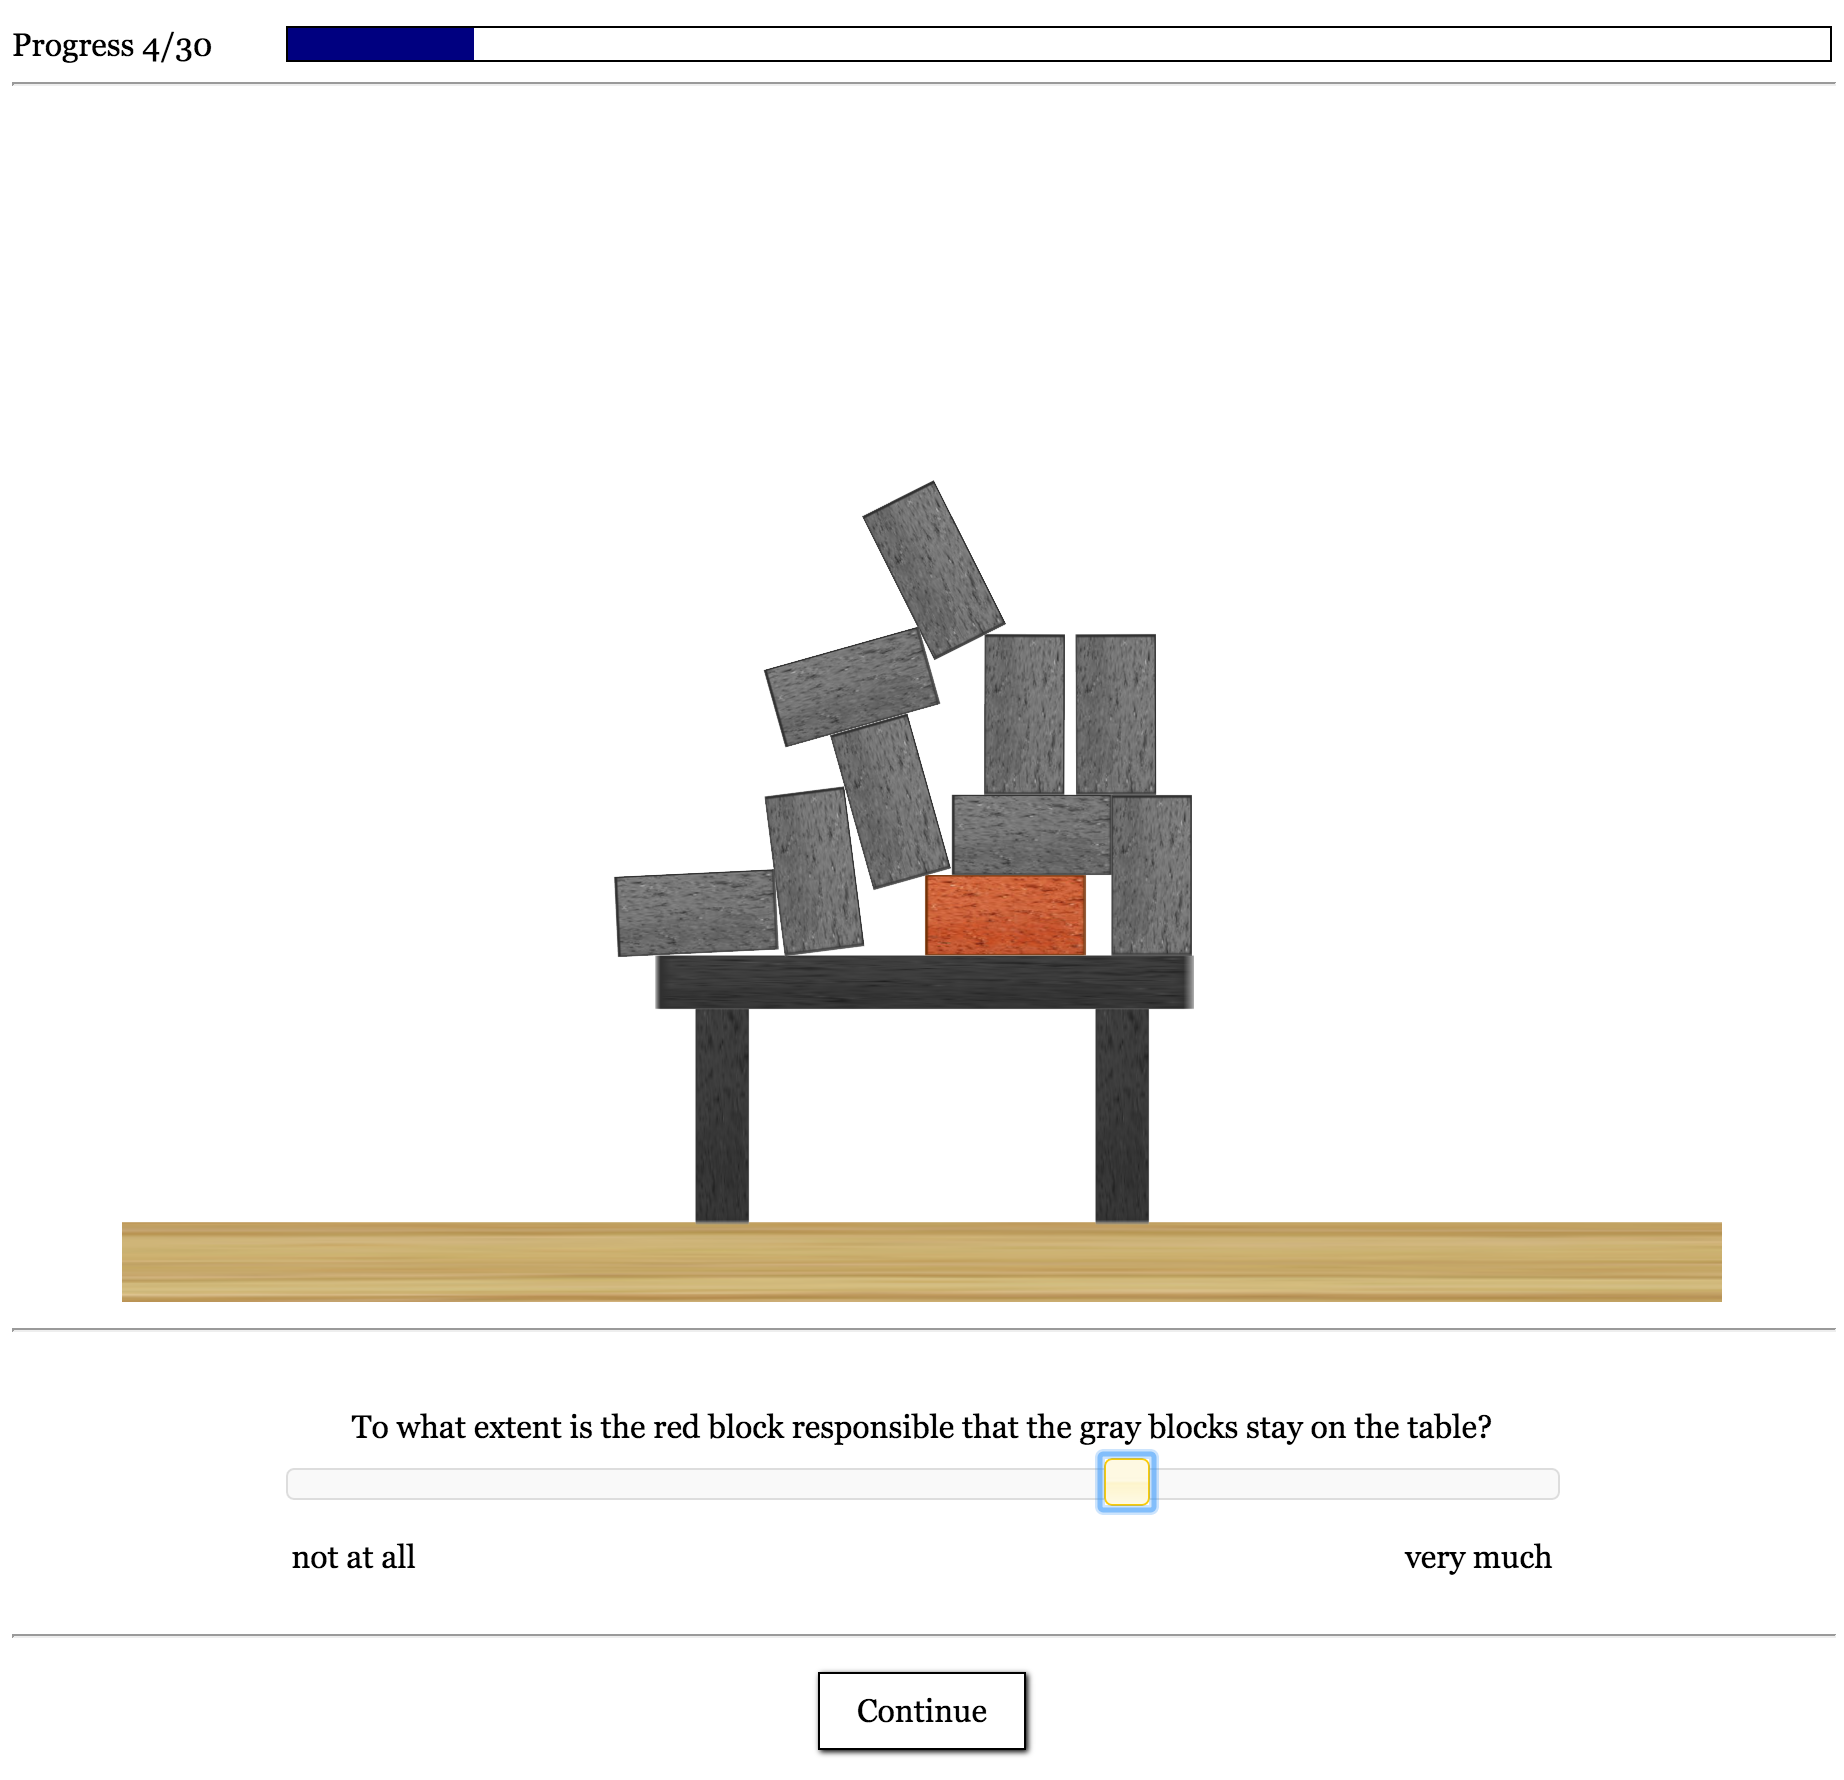
\includegraphics[width=0.32\columnwidth]{exp1_screenshot_3}}
% {\hfill}
% \caption{Experiment screenshots.}
% \label{fig:label}
% \end{figure}

% \begin{itemize}
%   \item Participants viewed a couple of animations of bricks falling on the table to get a sense for their physical properties. 
%   \item Participants then judged the responsibility of the red block for a set of 30 different stimuli (Figure~\ref{fig:Stimuli}).
% \end{itemize}

% \subsubsection{Stimuli}
% \label{sssec:stimuli}

% \begin{figure}[H]
% % \captionsetup[subfigure]{labelformat=empty}
% \renewcommand{\thesubfigure}{\arabic{subfigure}}
% \centering
% {\hfill}
% \subfloat[][bricks before: \textbf{9} (image~1)]{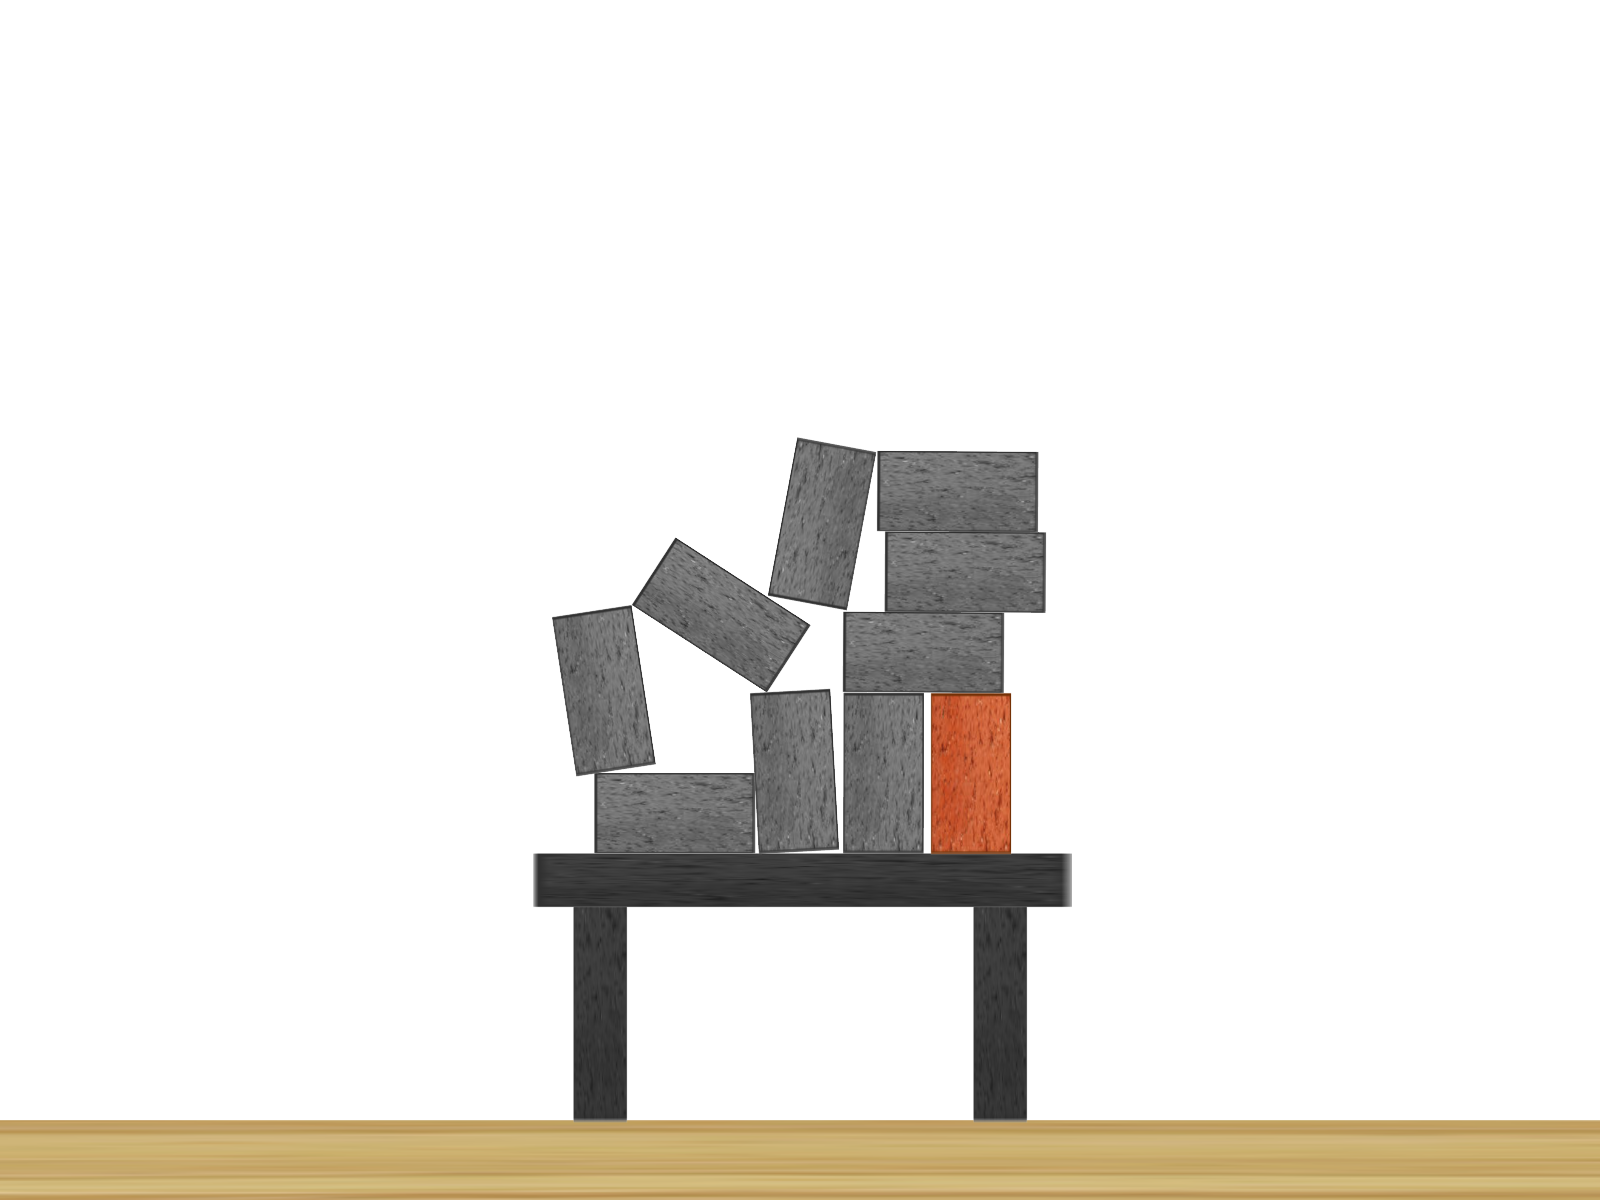
\includegraphics[width=0.2\columnwidth]{tower_image_(1)}}
% \hfill
% \subfloat[][bricks before: \textbf{9} (image~2)]{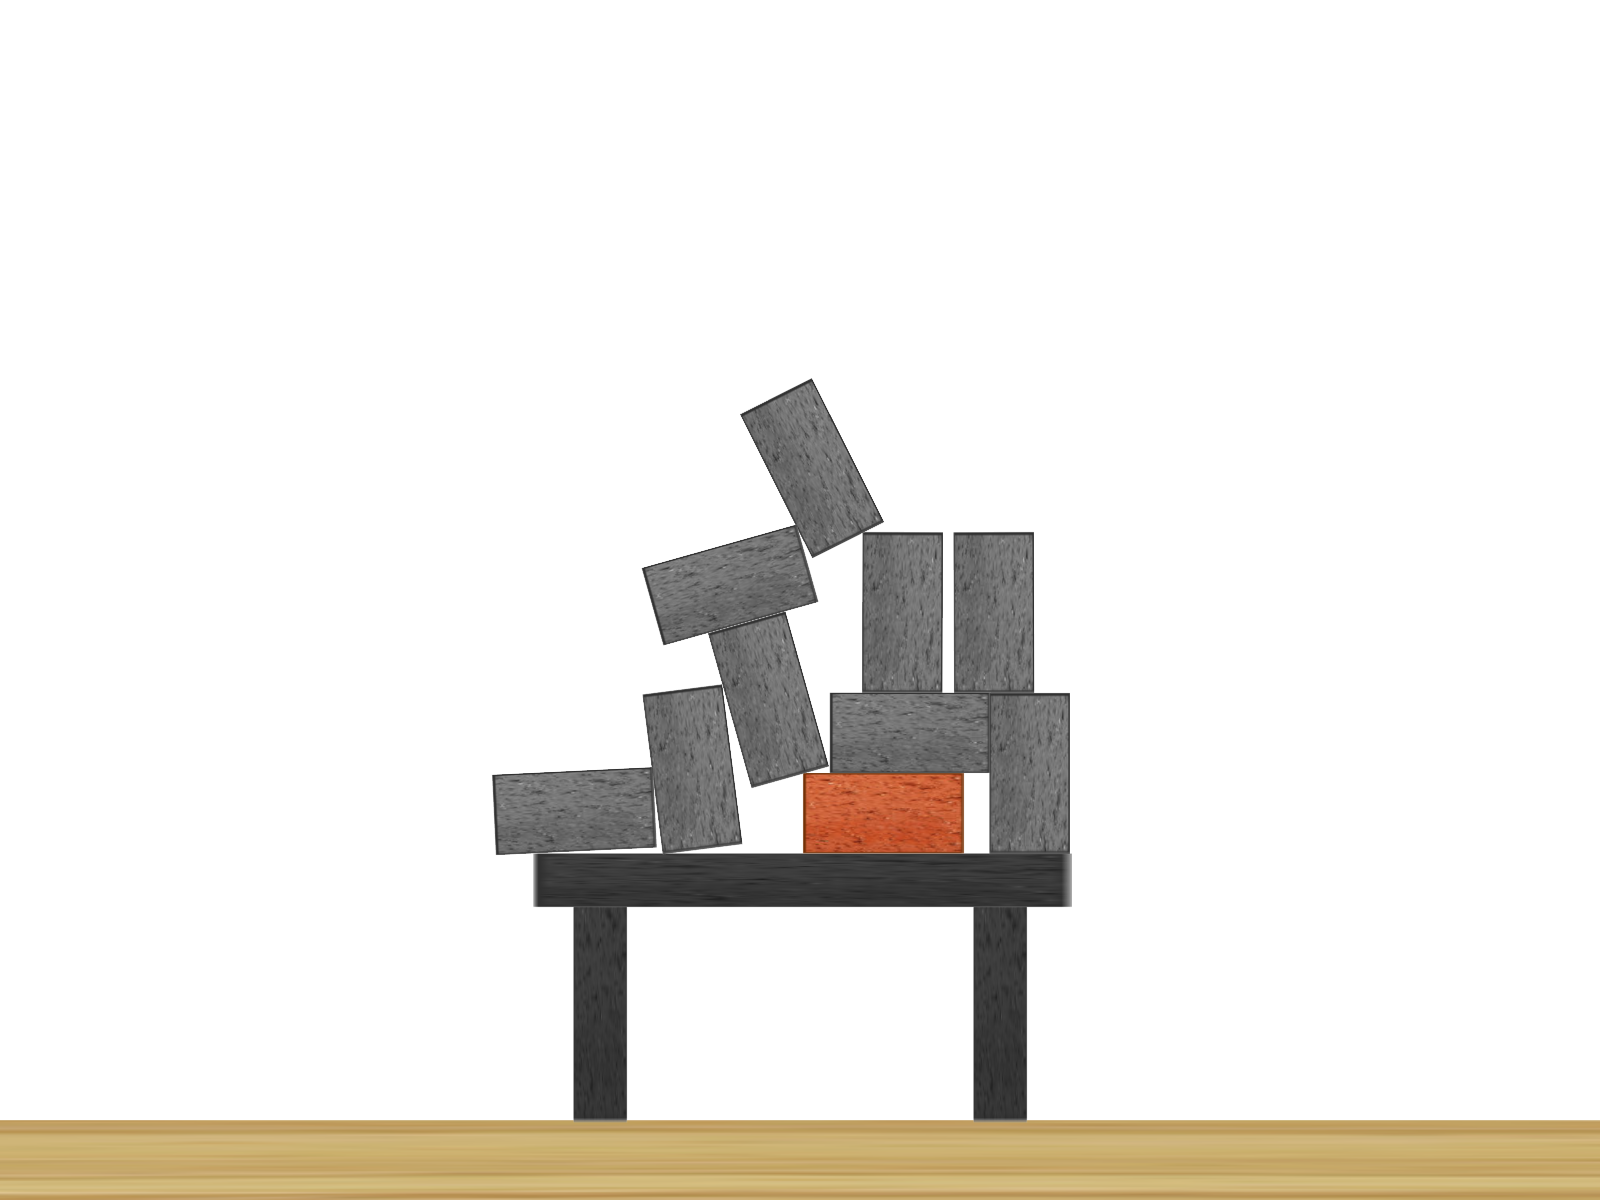
\includegraphics[width=0.2\columnwidth]{tower_image_(2)}}
% \hfill
% \subfloat[][bricks before: \textbf{18} (image~4)]{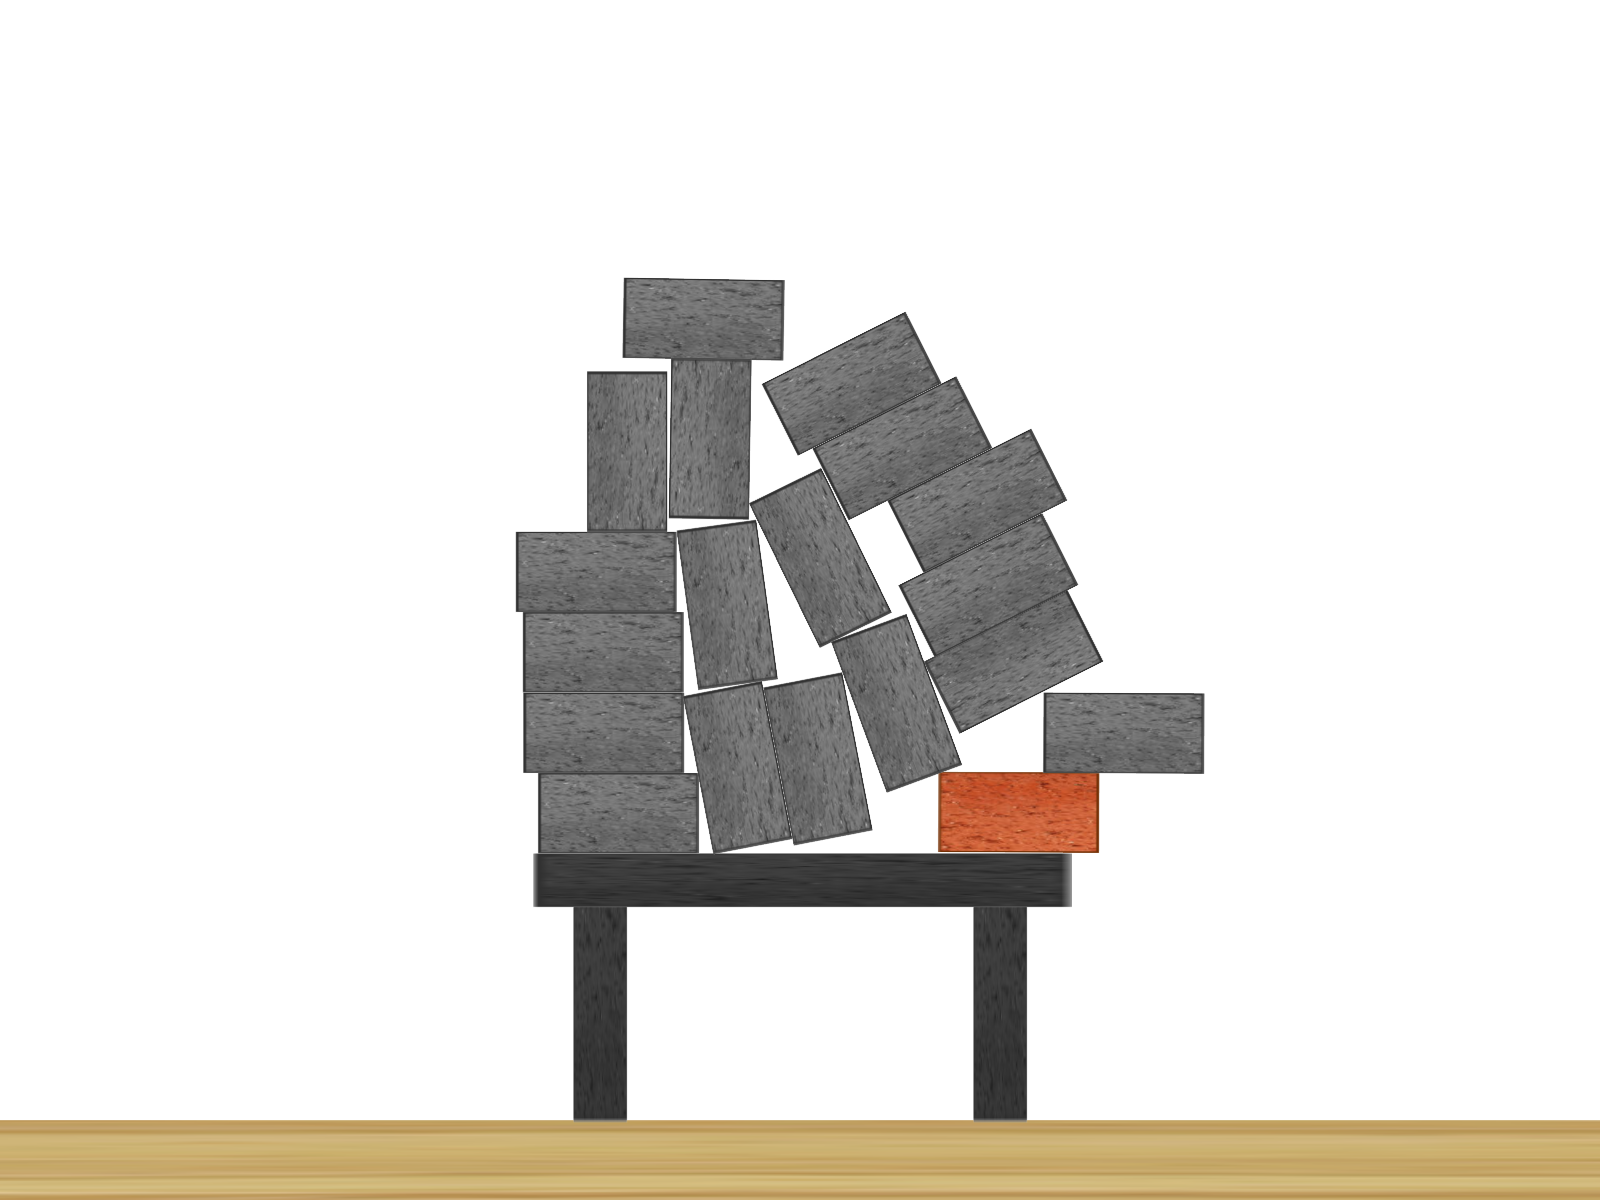
\includegraphics[width=0.2\columnwidth]{tower_image_(4)}}
% \hfill
% \subfloat[][bricks before: \textbf{3} (image~5)]{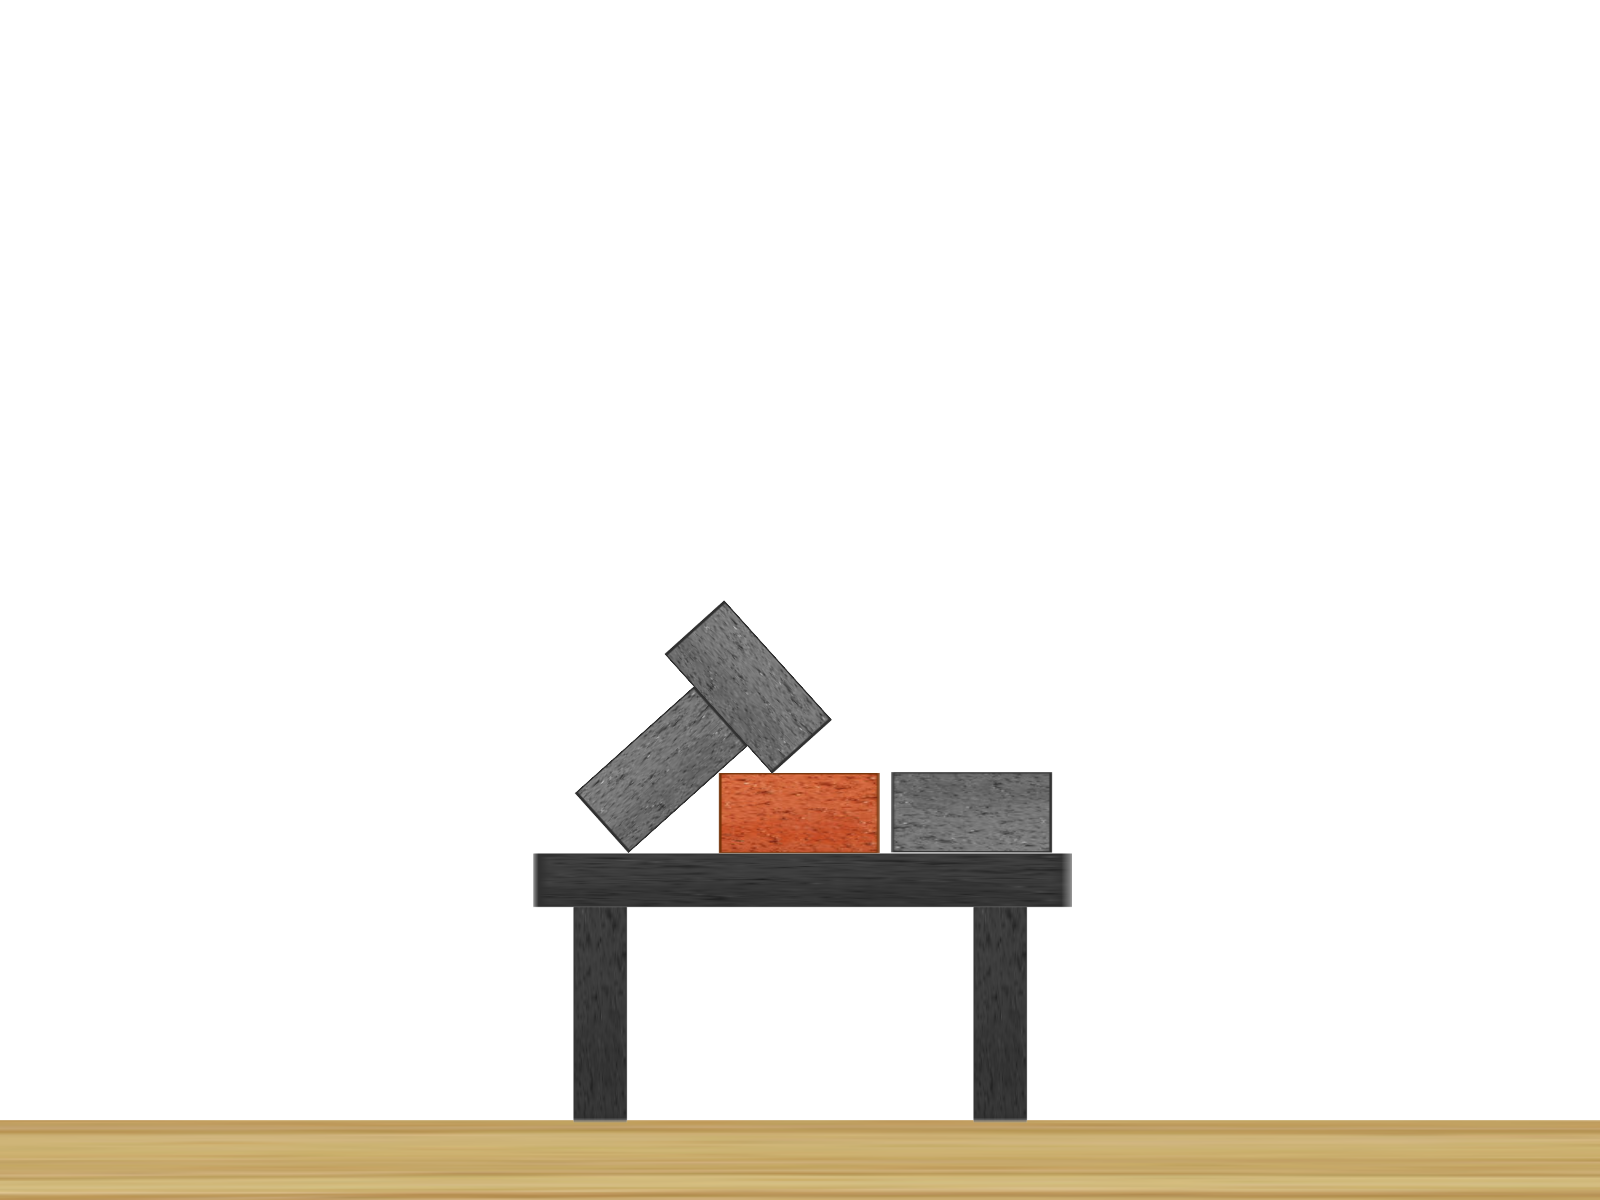
\includegraphics[width=0.2\columnwidth]{tower_image_(5)}}
% {\hfill}

% {\hfill}
% \subfloat[][bricks before: \textbf{7} (image~6)]{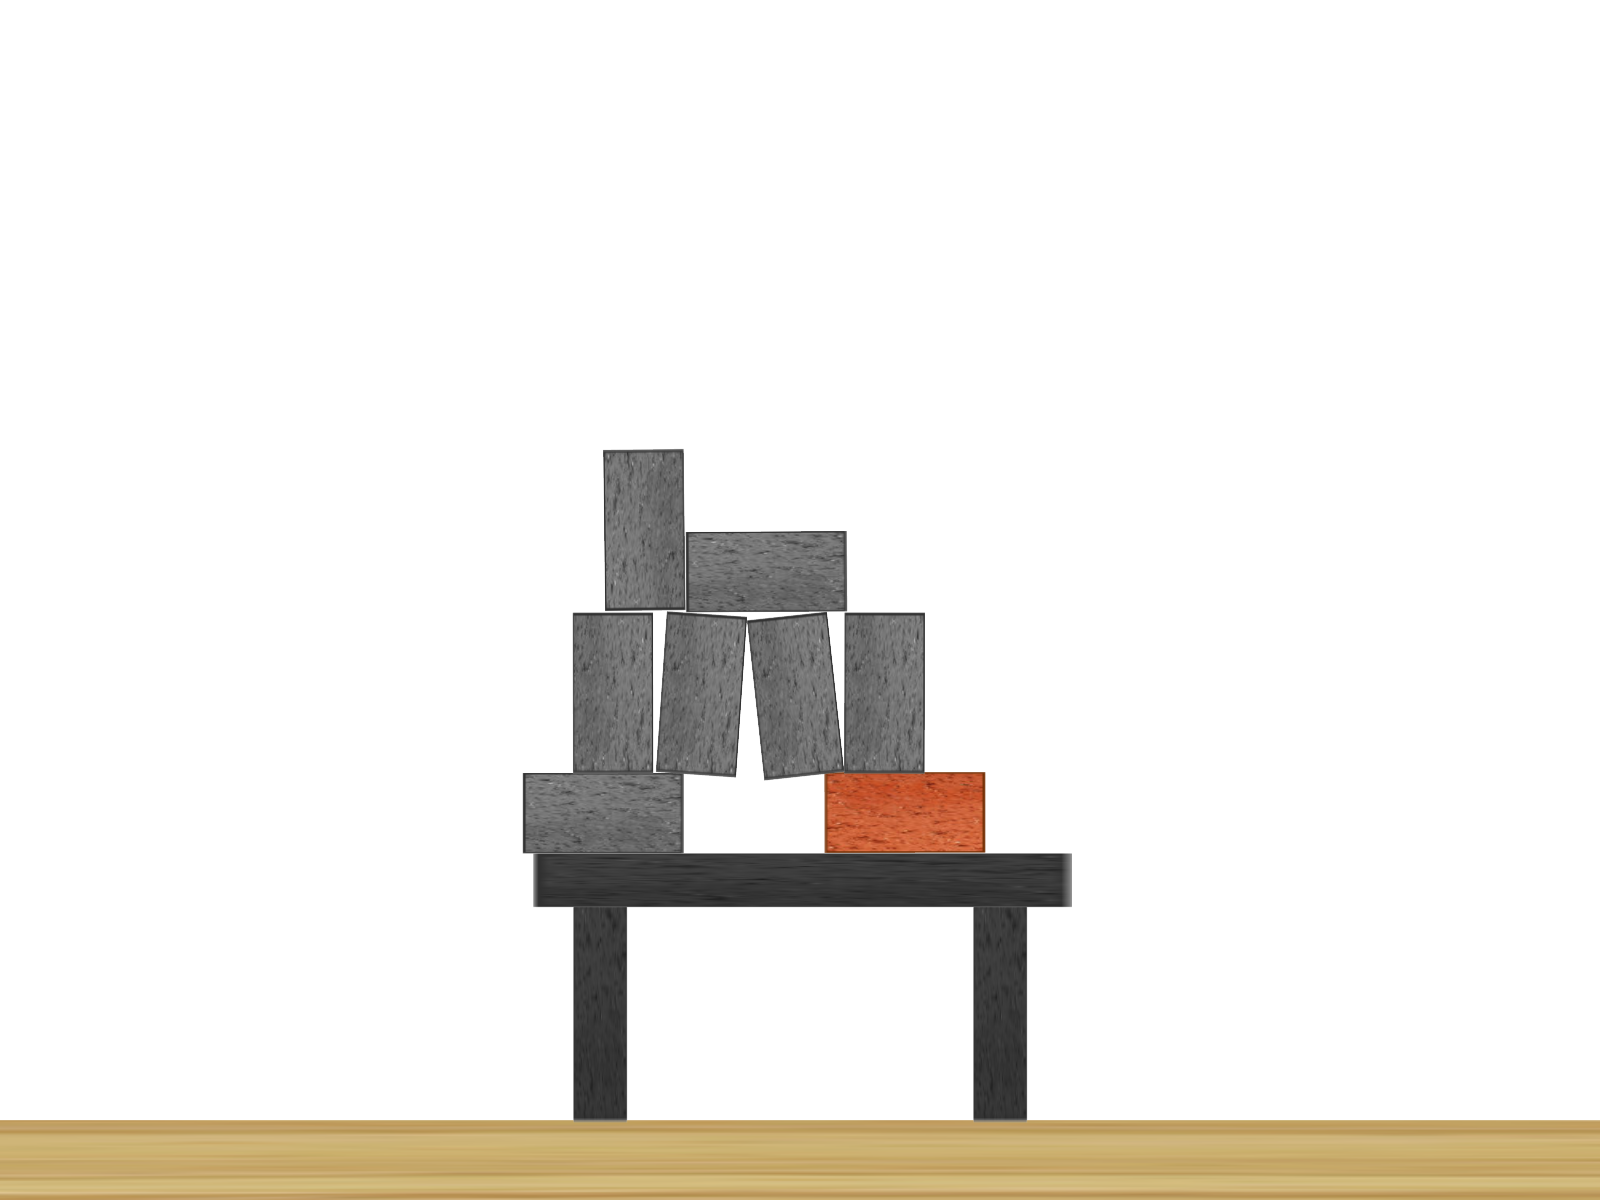
\includegraphics[width=0.2\columnwidth]{tower_image_(6)}}
% \hfill
% \subfloat[][bricks before: \textbf{3} (image~7)]{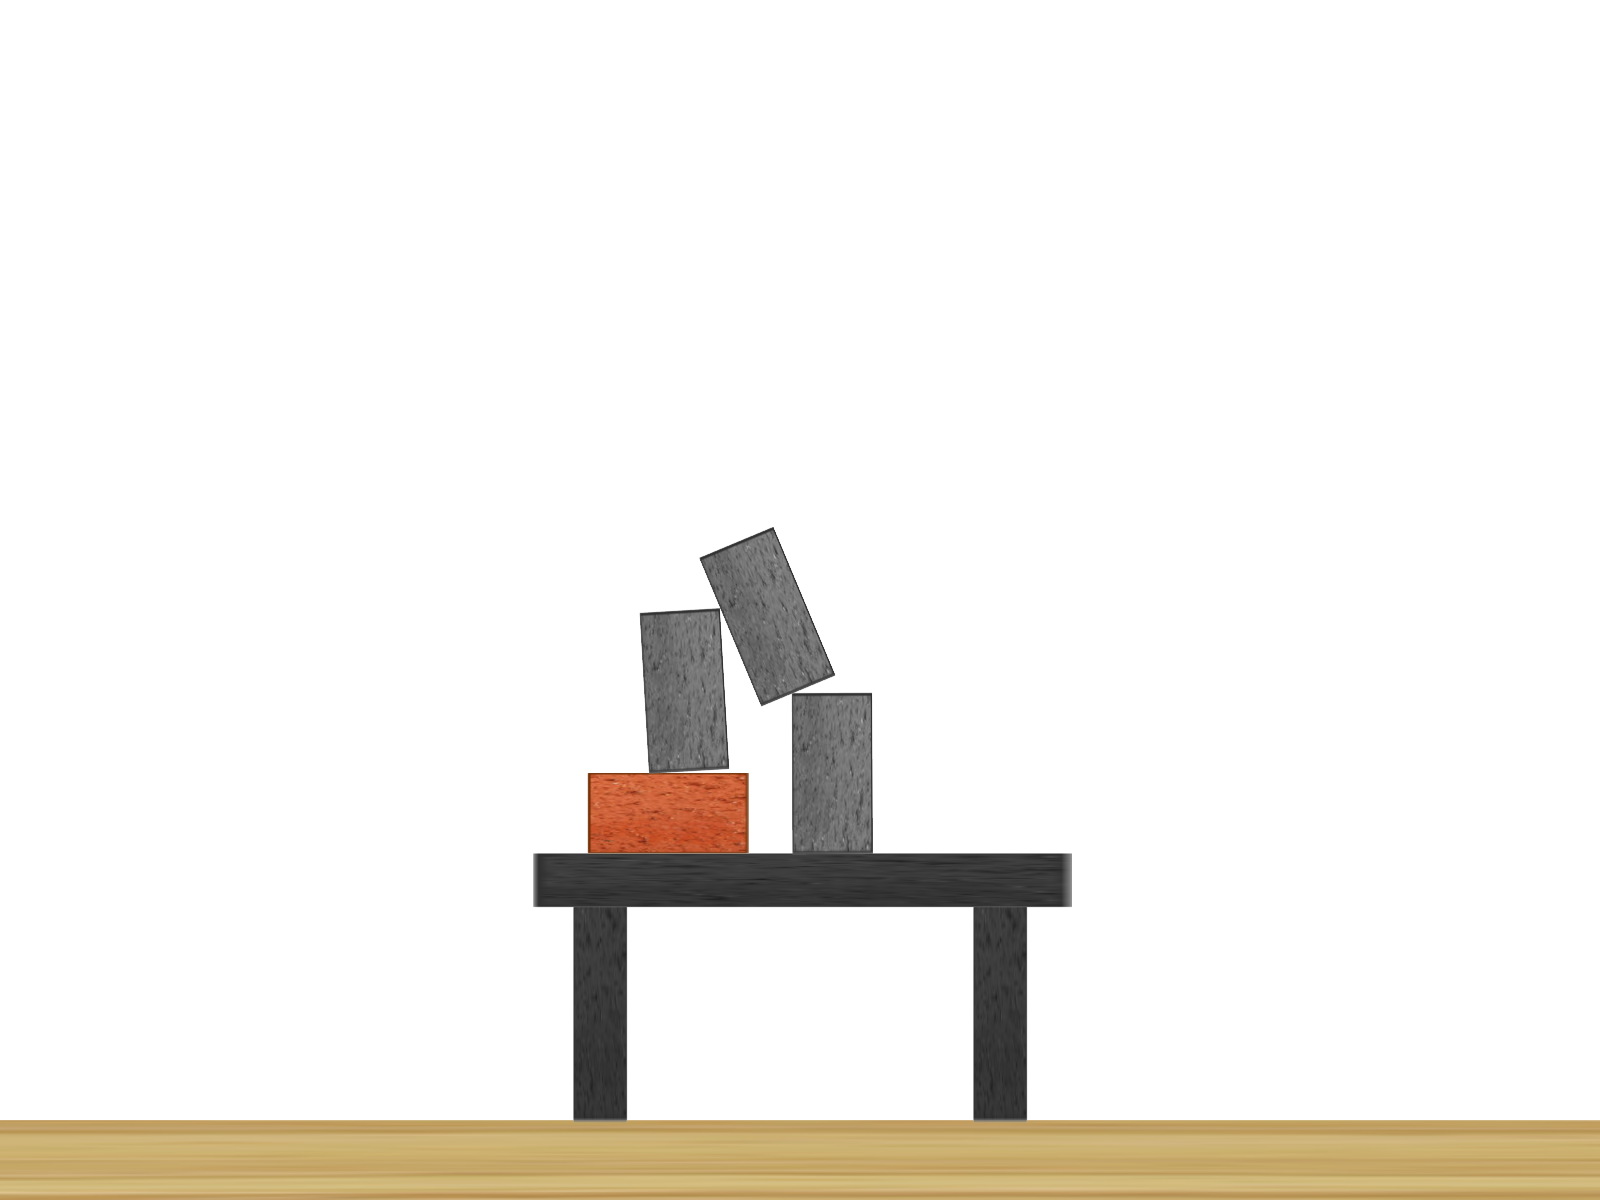
\includegraphics[width=0.2\columnwidth]{tower_image_(7)}}
% \hfill
% \subfloat[][bricks before: \textbf{7} (image~8)]{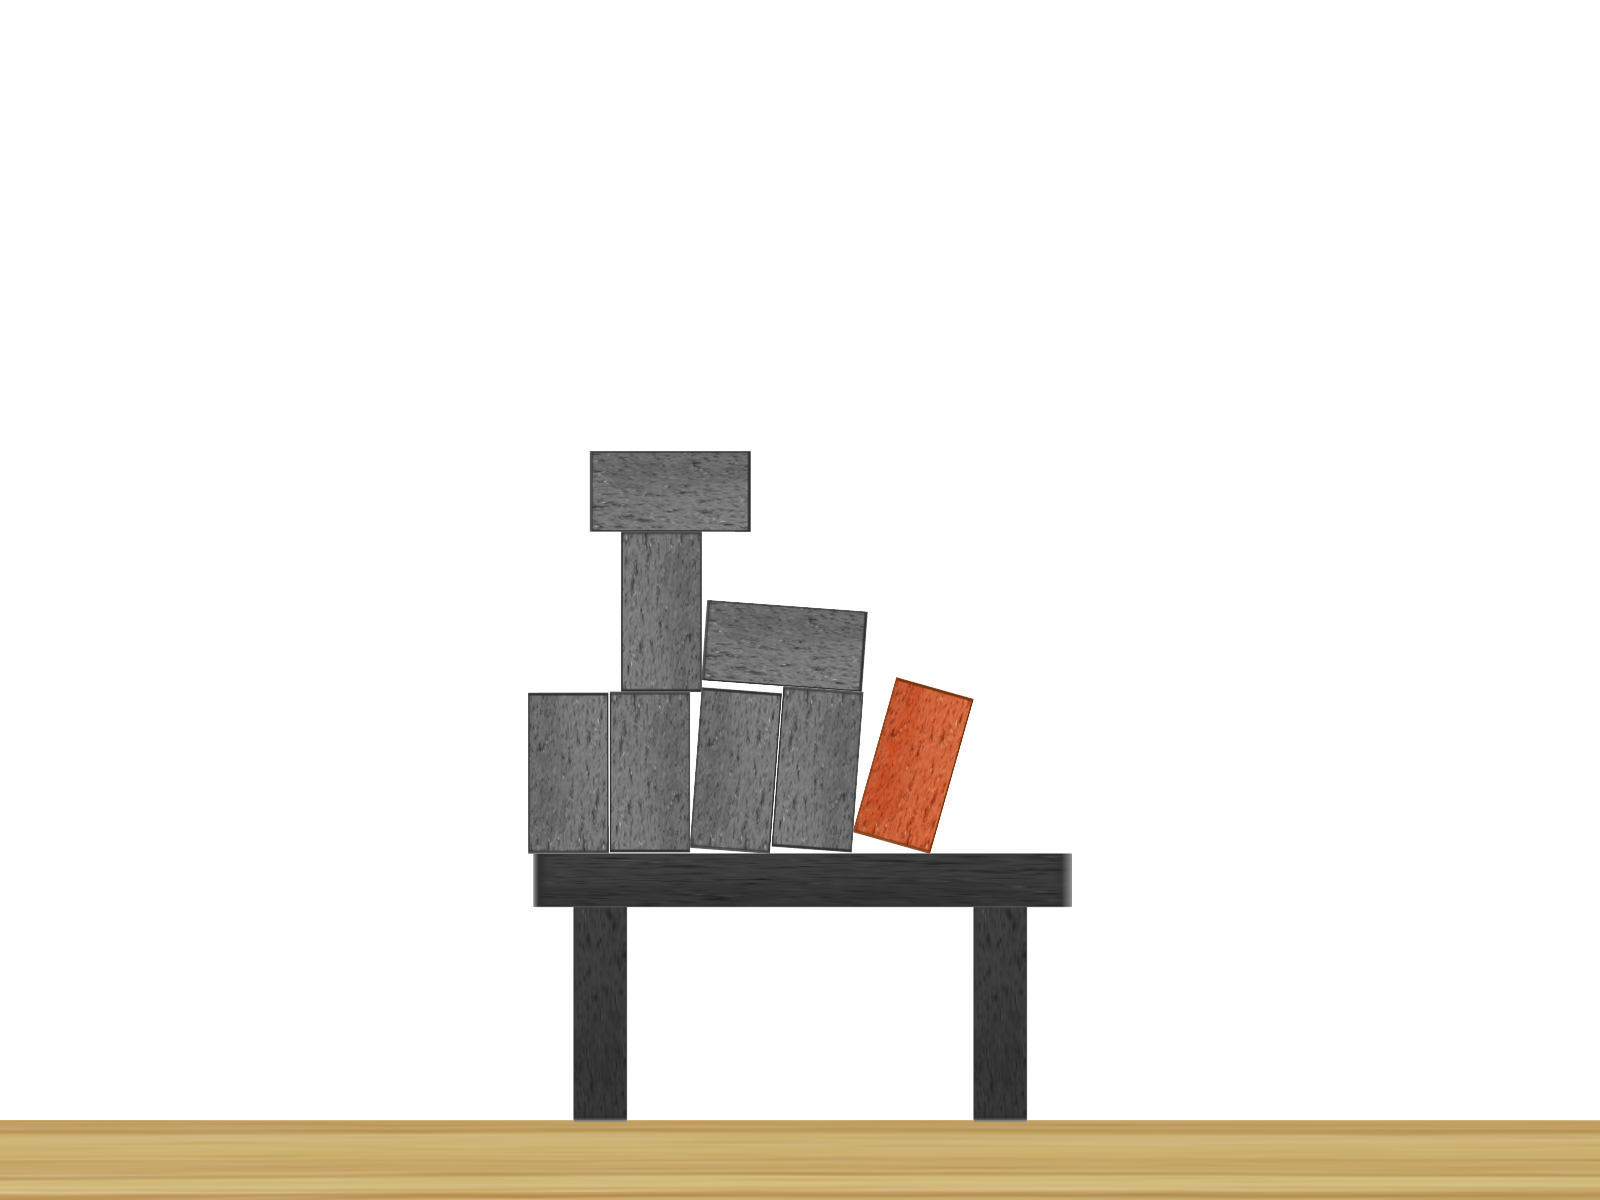
\includegraphics[width=0.2\columnwidth]{tower_image_(8)}}
% \hfill
% \subfloat[][bricks before: \textbf{5} (image~13)]{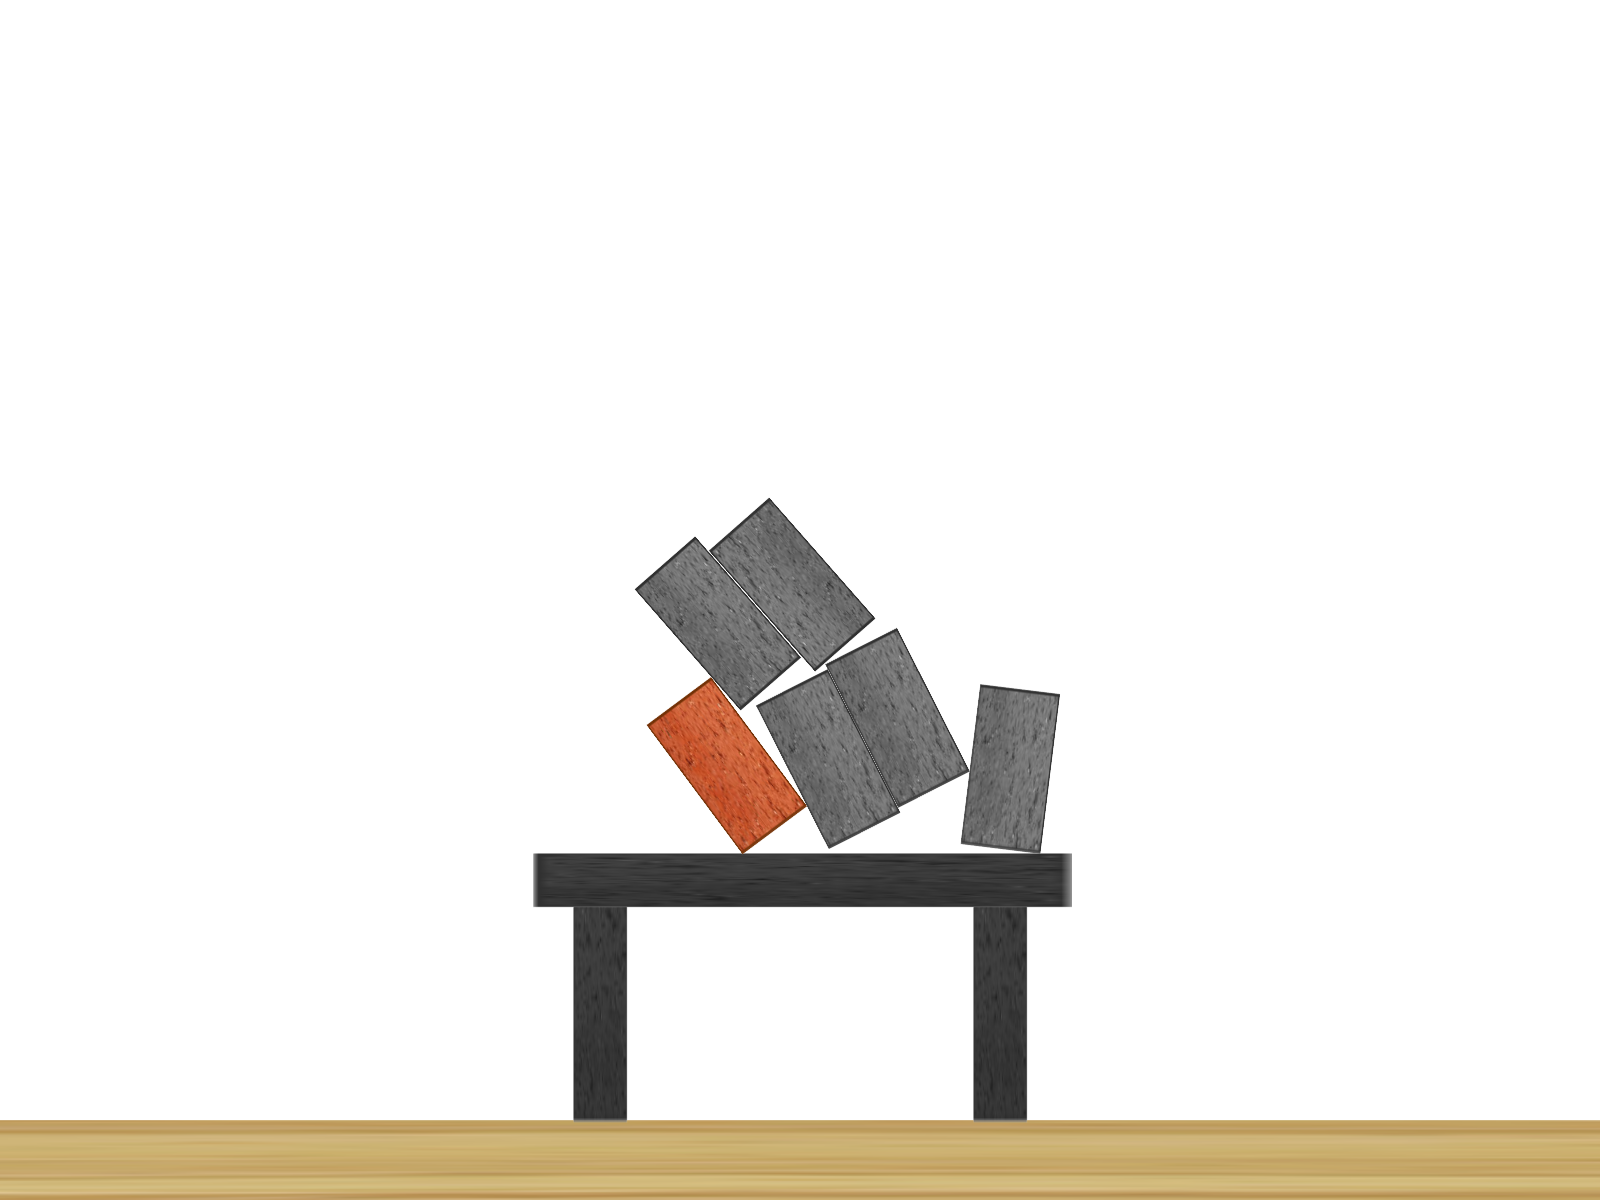
\includegraphics[width=0.2\columnwidth]{tower_image_(13)}}
% {\hfill}

% {\hfill}
% \subfloat[][bricks before: \textbf{6} (image~14)]{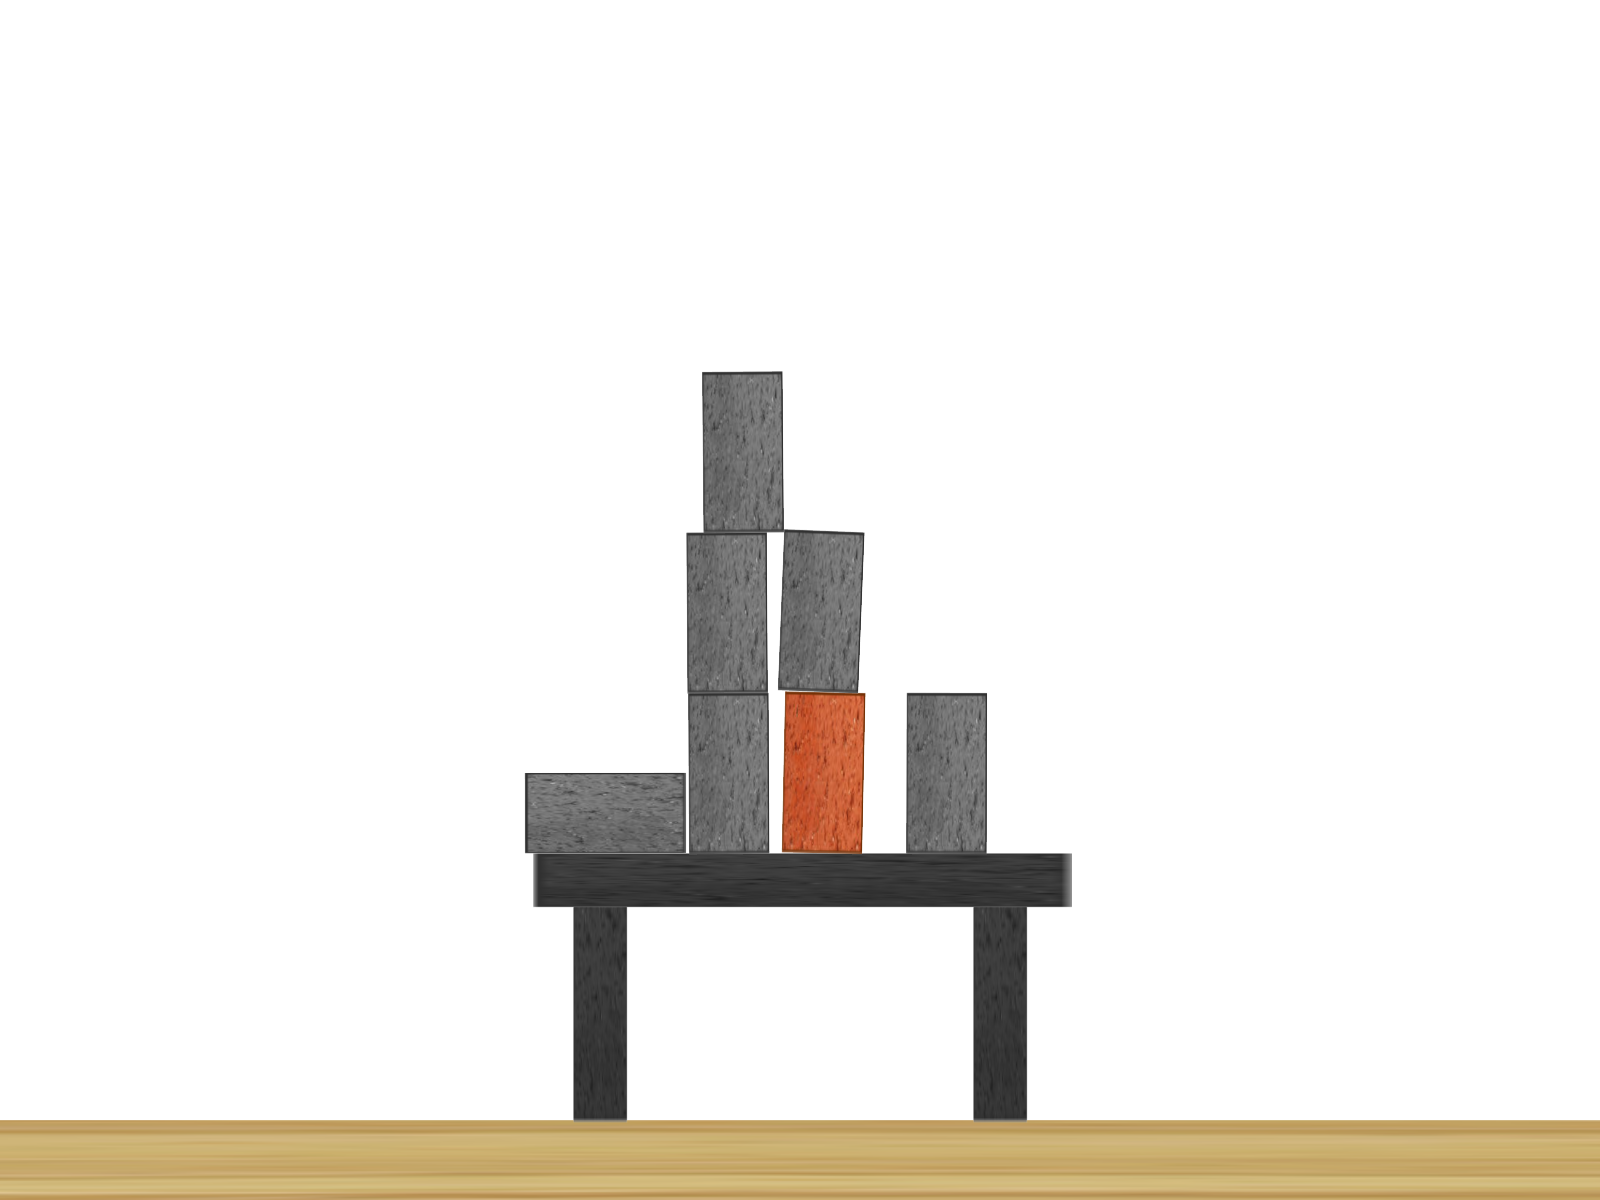
\includegraphics[width=0.2\columnwidth]{tower_image_(14)}}
% \hfill
% \subfloat[][bricks before: \textbf{12} (image~15)]{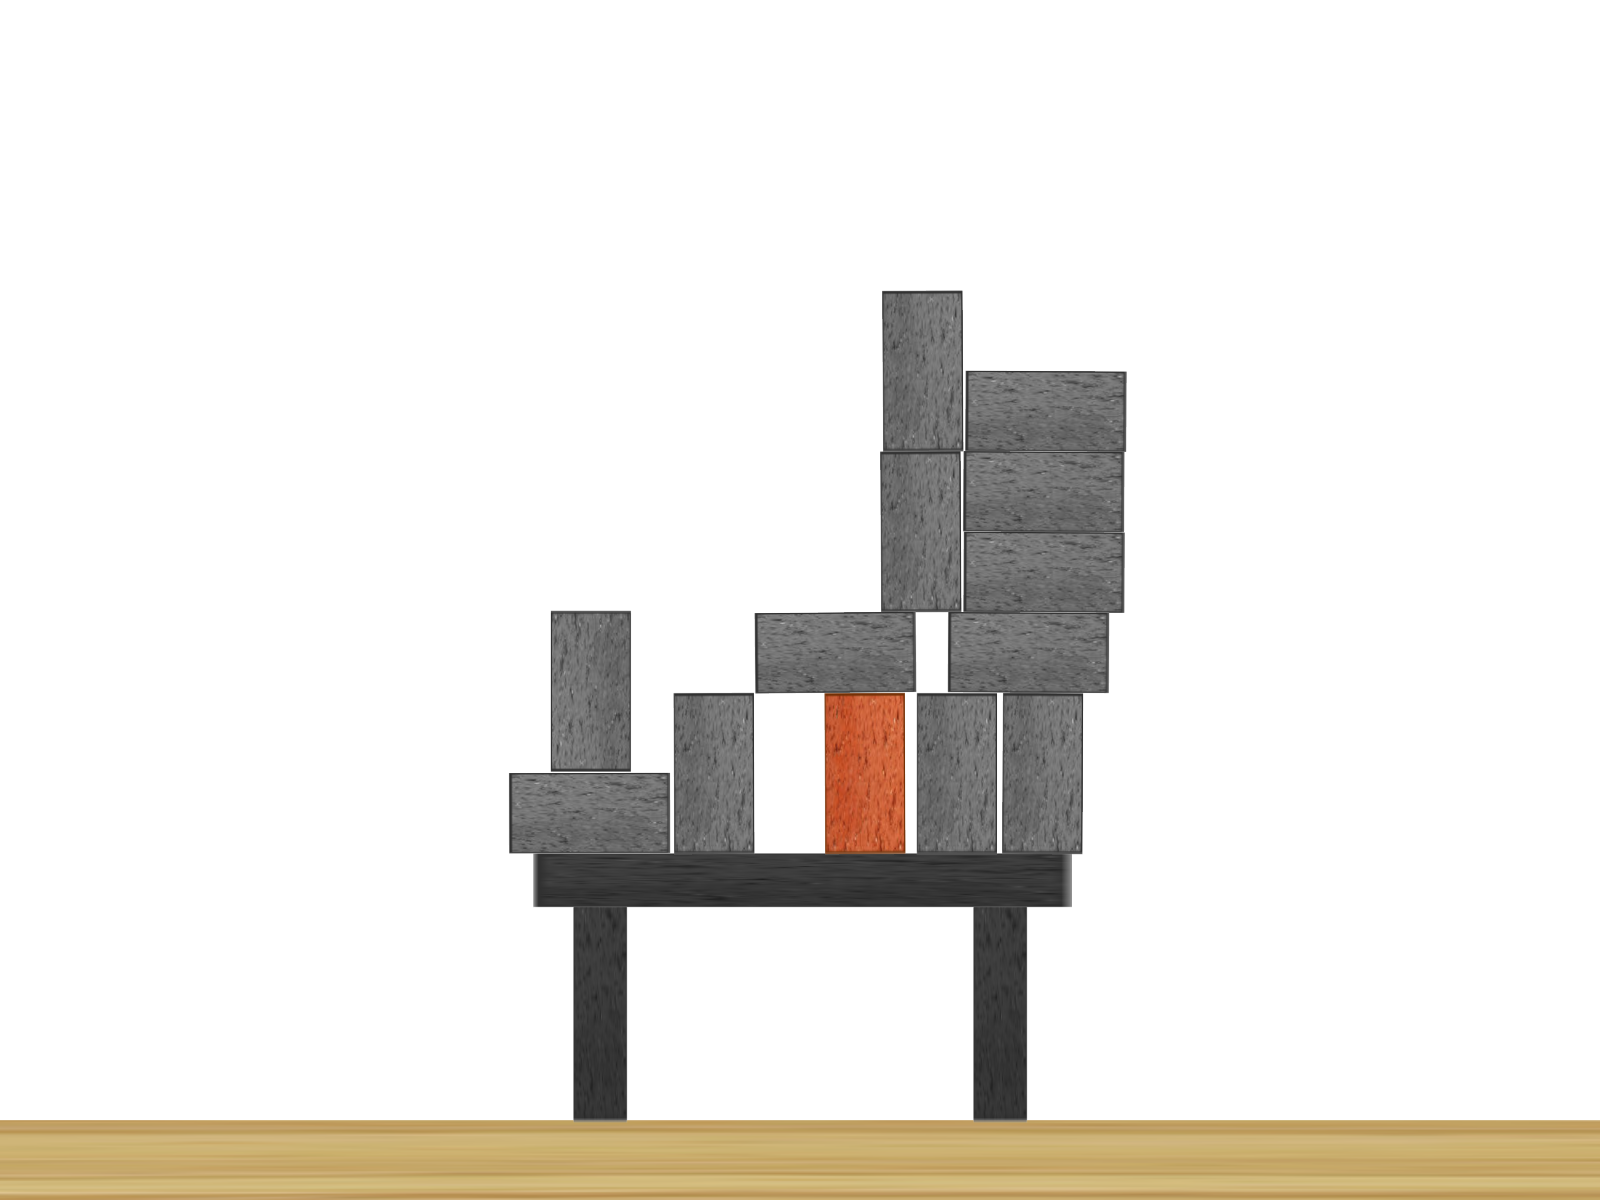
\includegraphics[width=0.2\columnwidth]{tower_image_(15)}}
% \hfill
% \subfloat[][bricks before: \textbf{3} (image~16)]{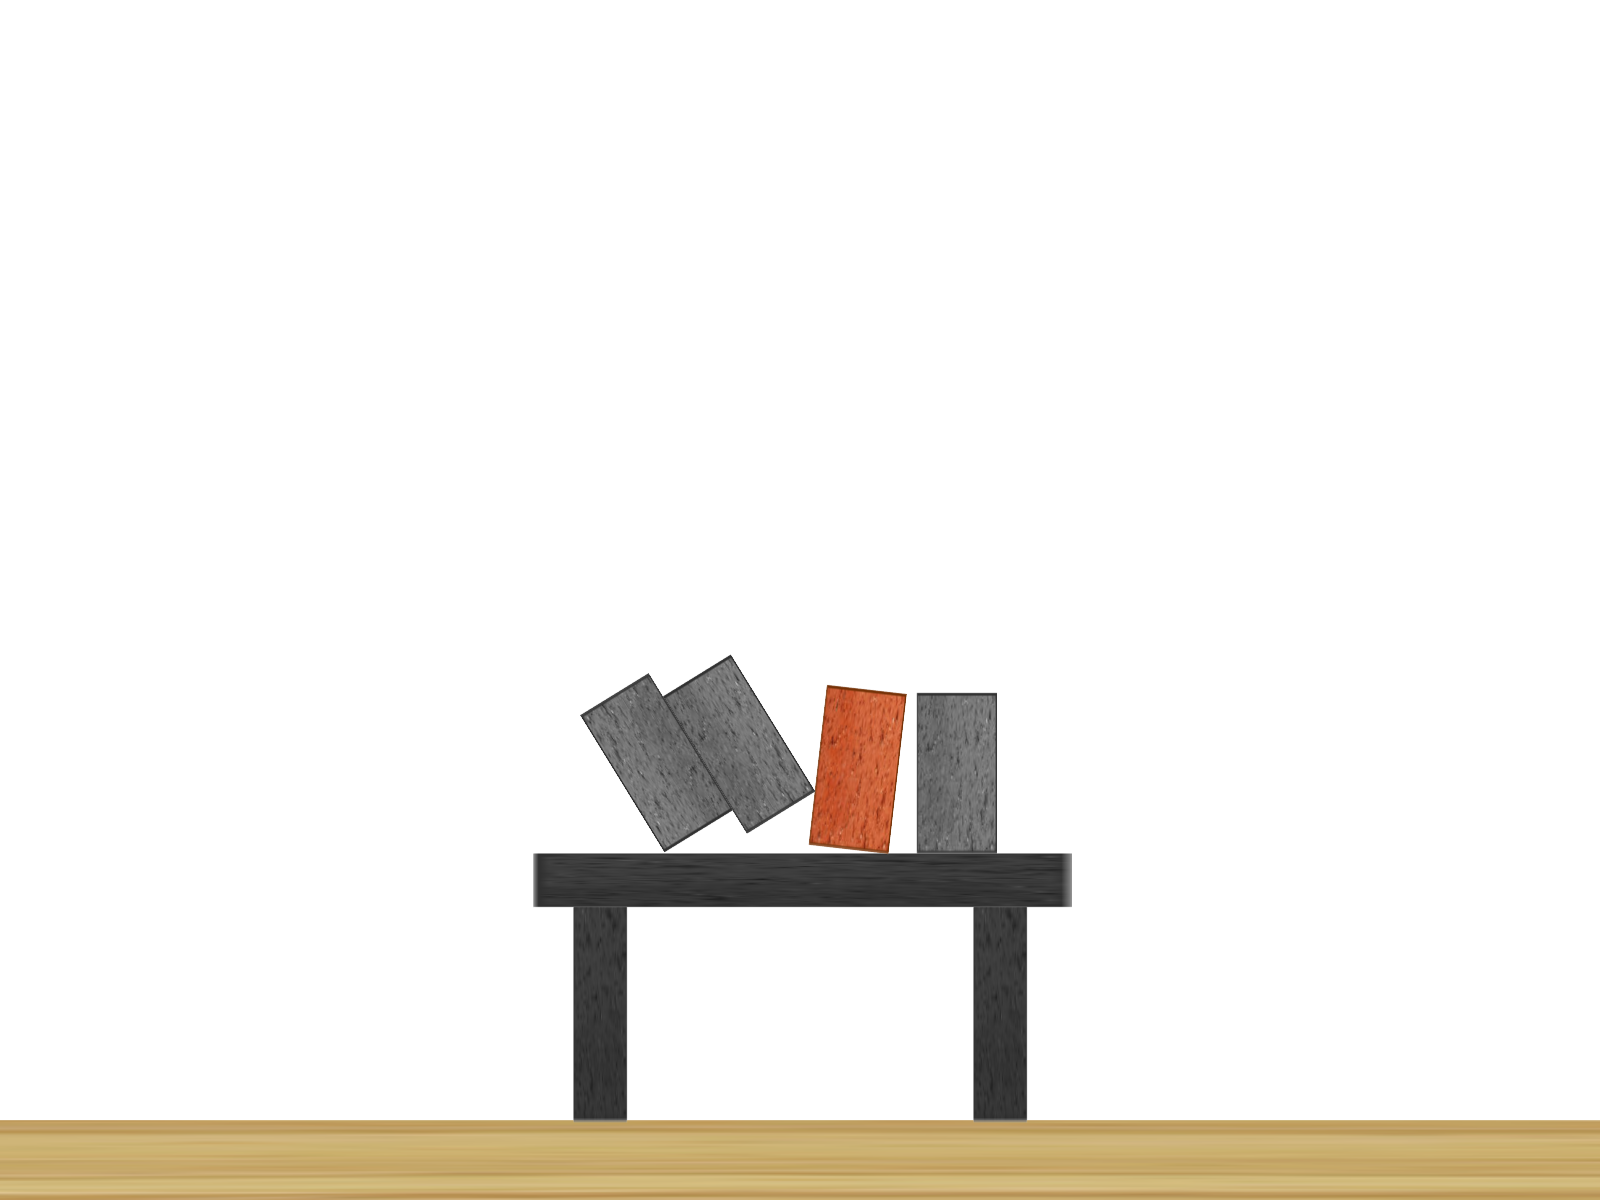
\includegraphics[width=0.2\columnwidth]{tower_image_(16)}}
% \hfill
% \subfloat[][bricks before: \textbf{3} (image~17)]{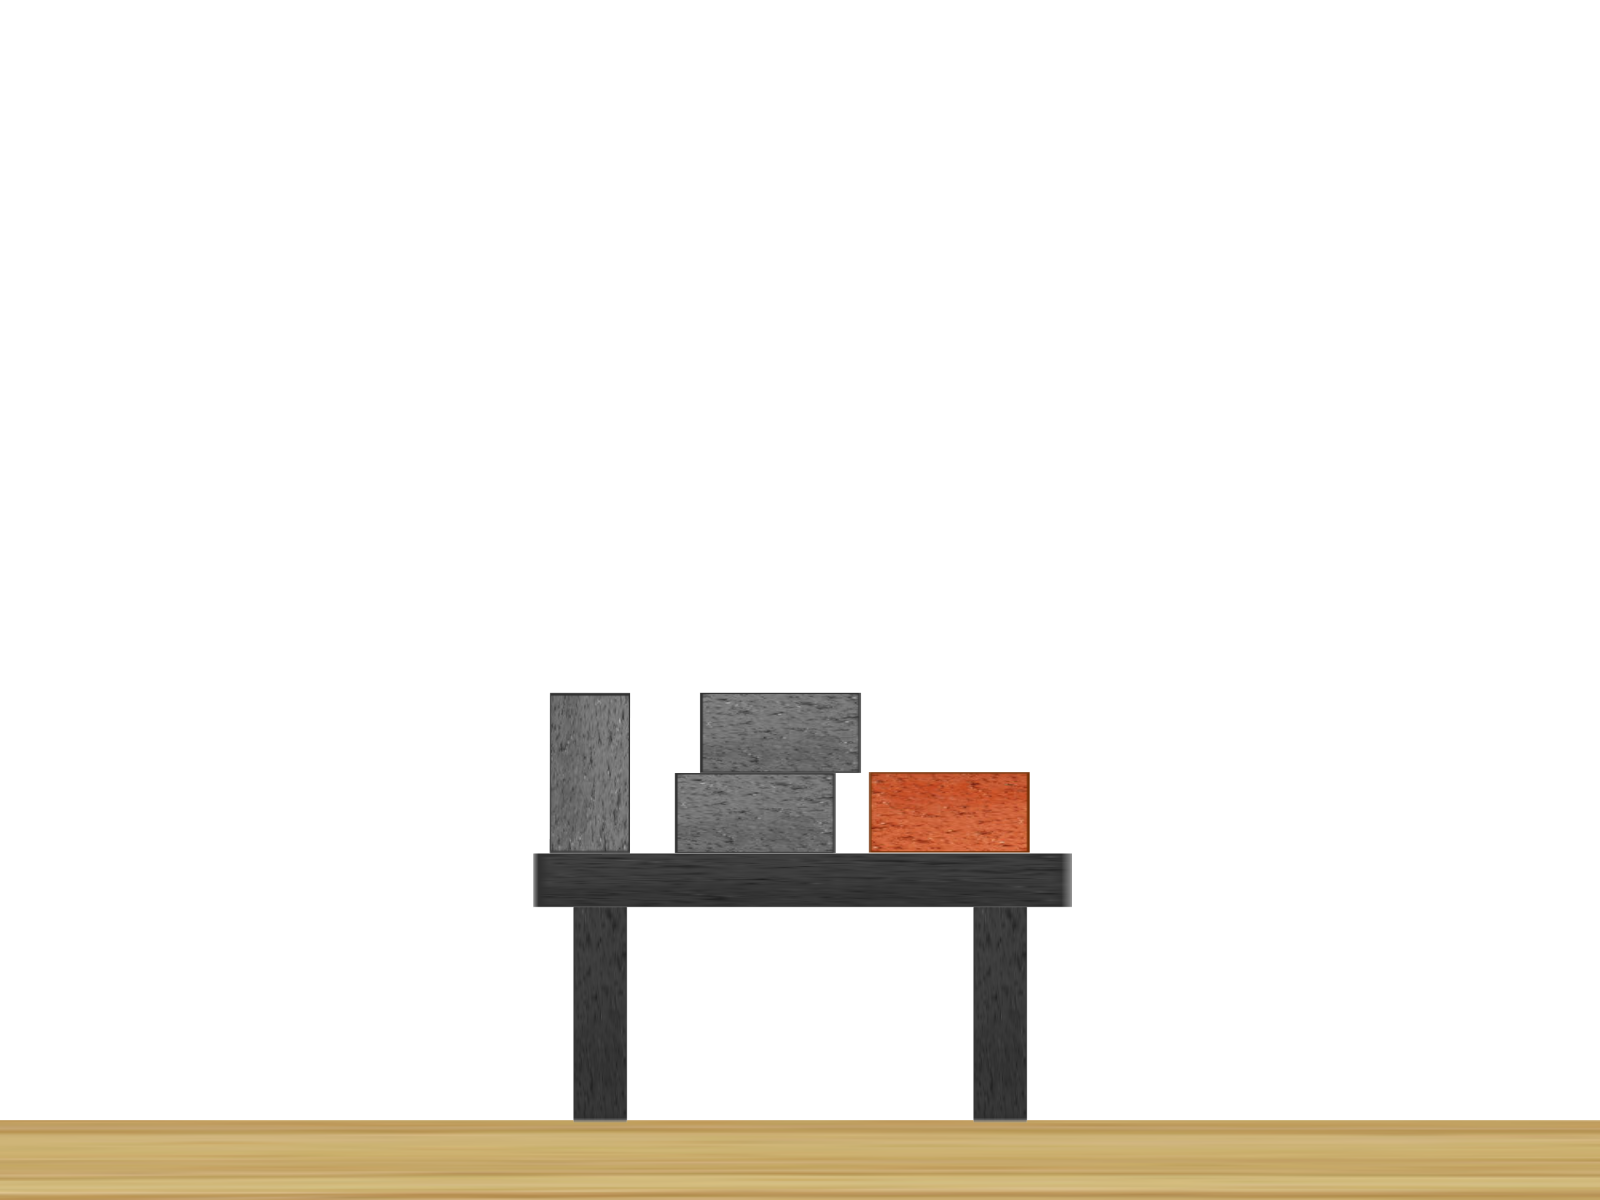
\includegraphics[width=0.2\columnwidth]{tower_image_(17)}}
% {\hfill}

% {\hfill}
% \subfloat[][bricks before: \textbf{5} (image~18)]{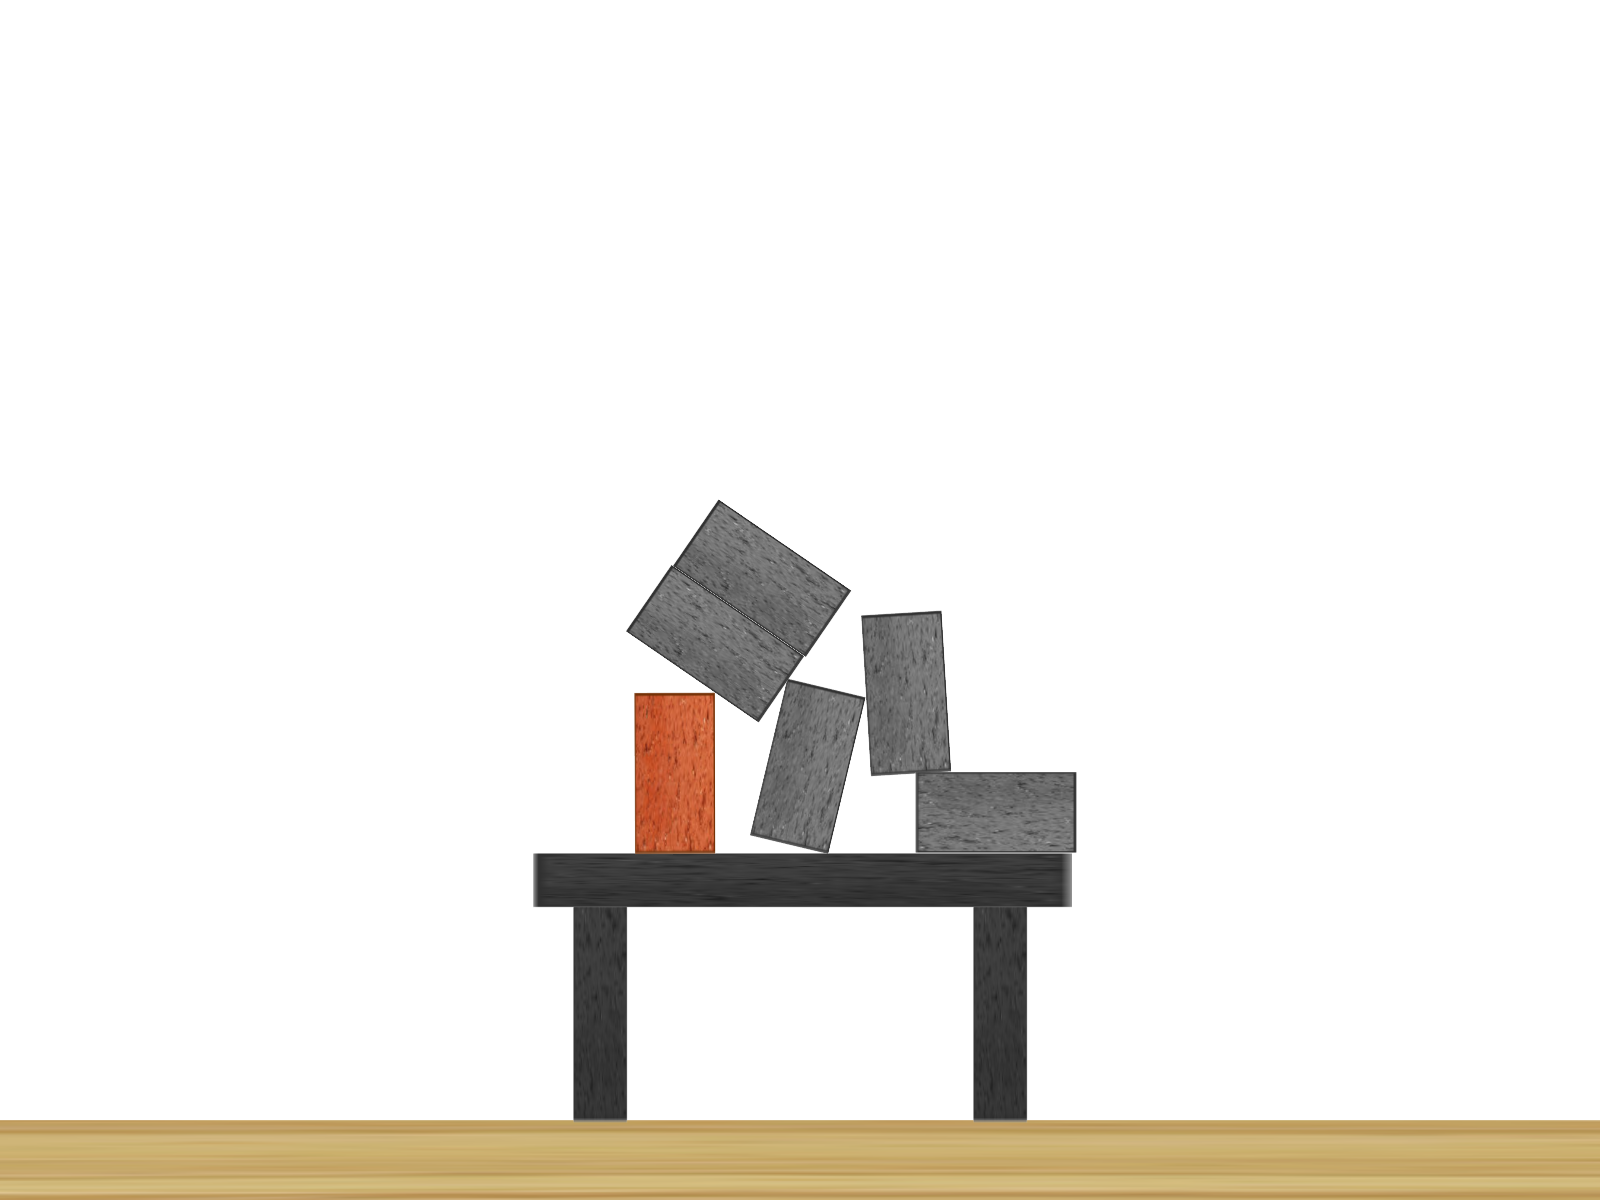
\includegraphics[width=0.2\columnwidth]{tower_image_(18)}}
% \hfill
% \subfloat[][bricks before: \textbf{11} (image~19)]{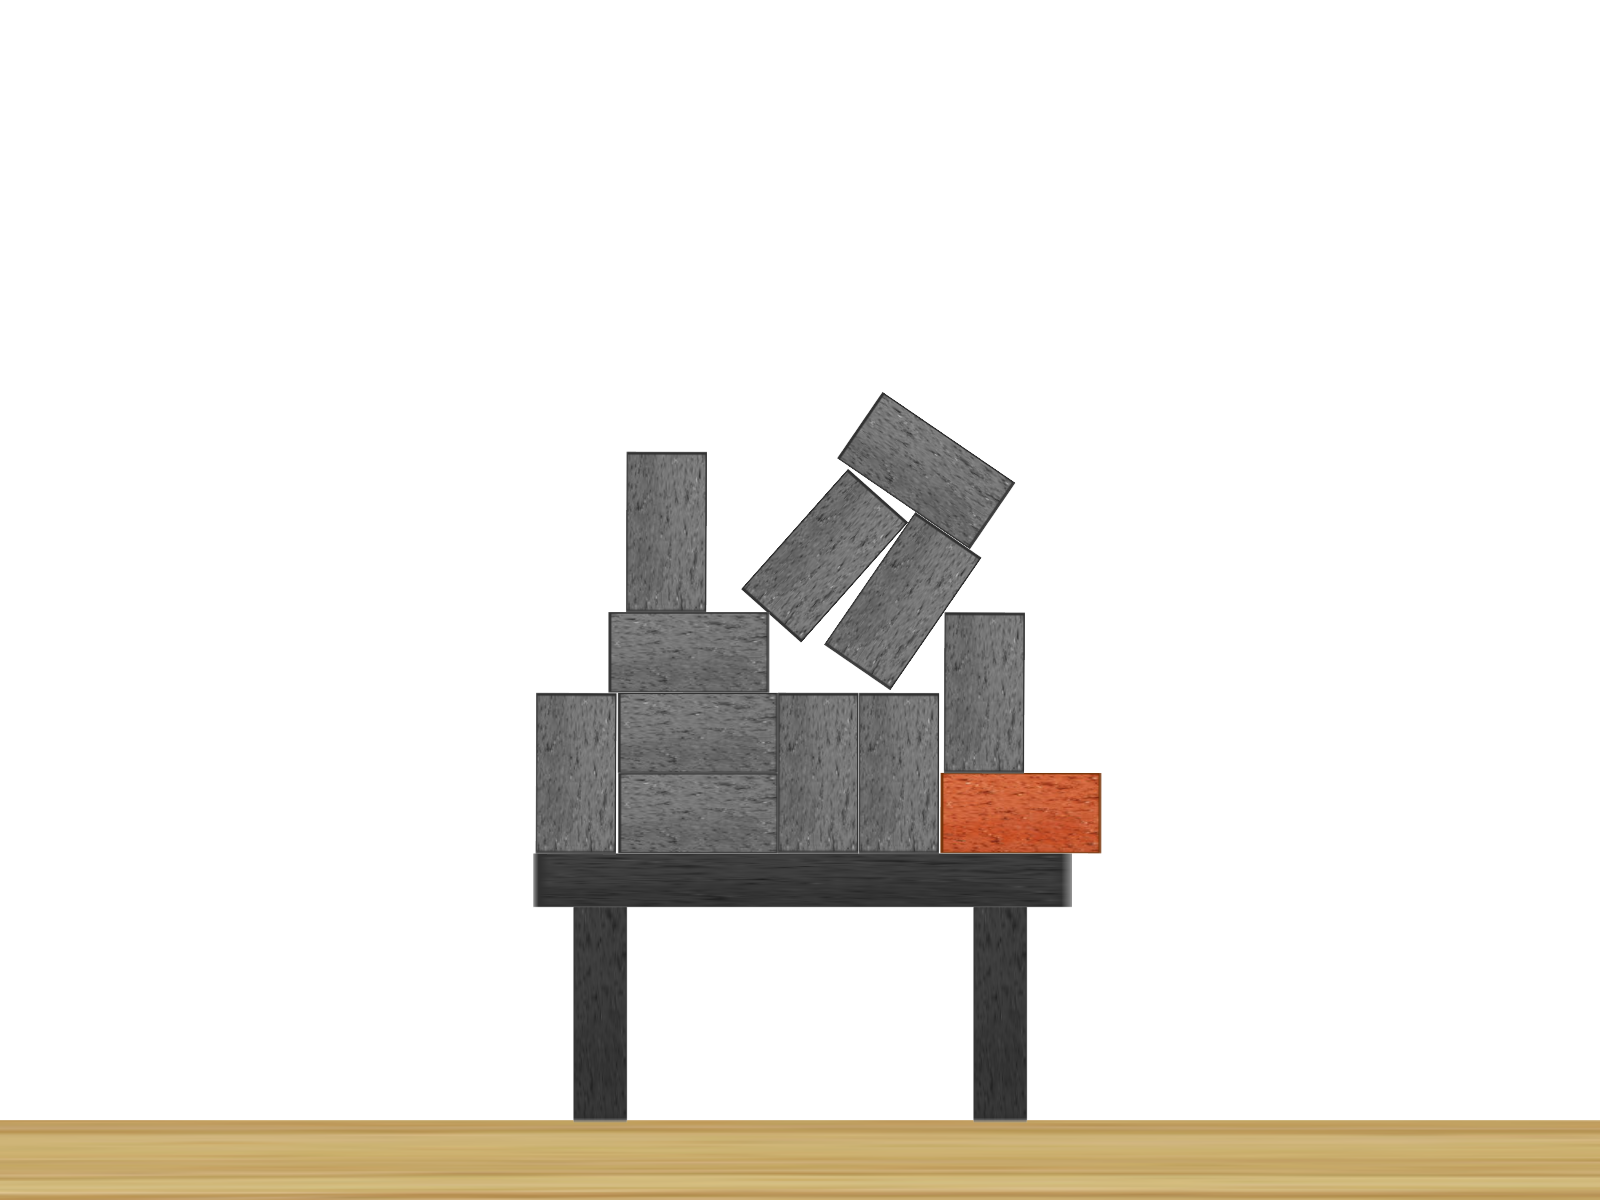
\includegraphics[width=0.2\columnwidth]{tower_image_(19)}}
% \hfill
% \subfloat[][bricks before: \textbf{8} (image~21)]{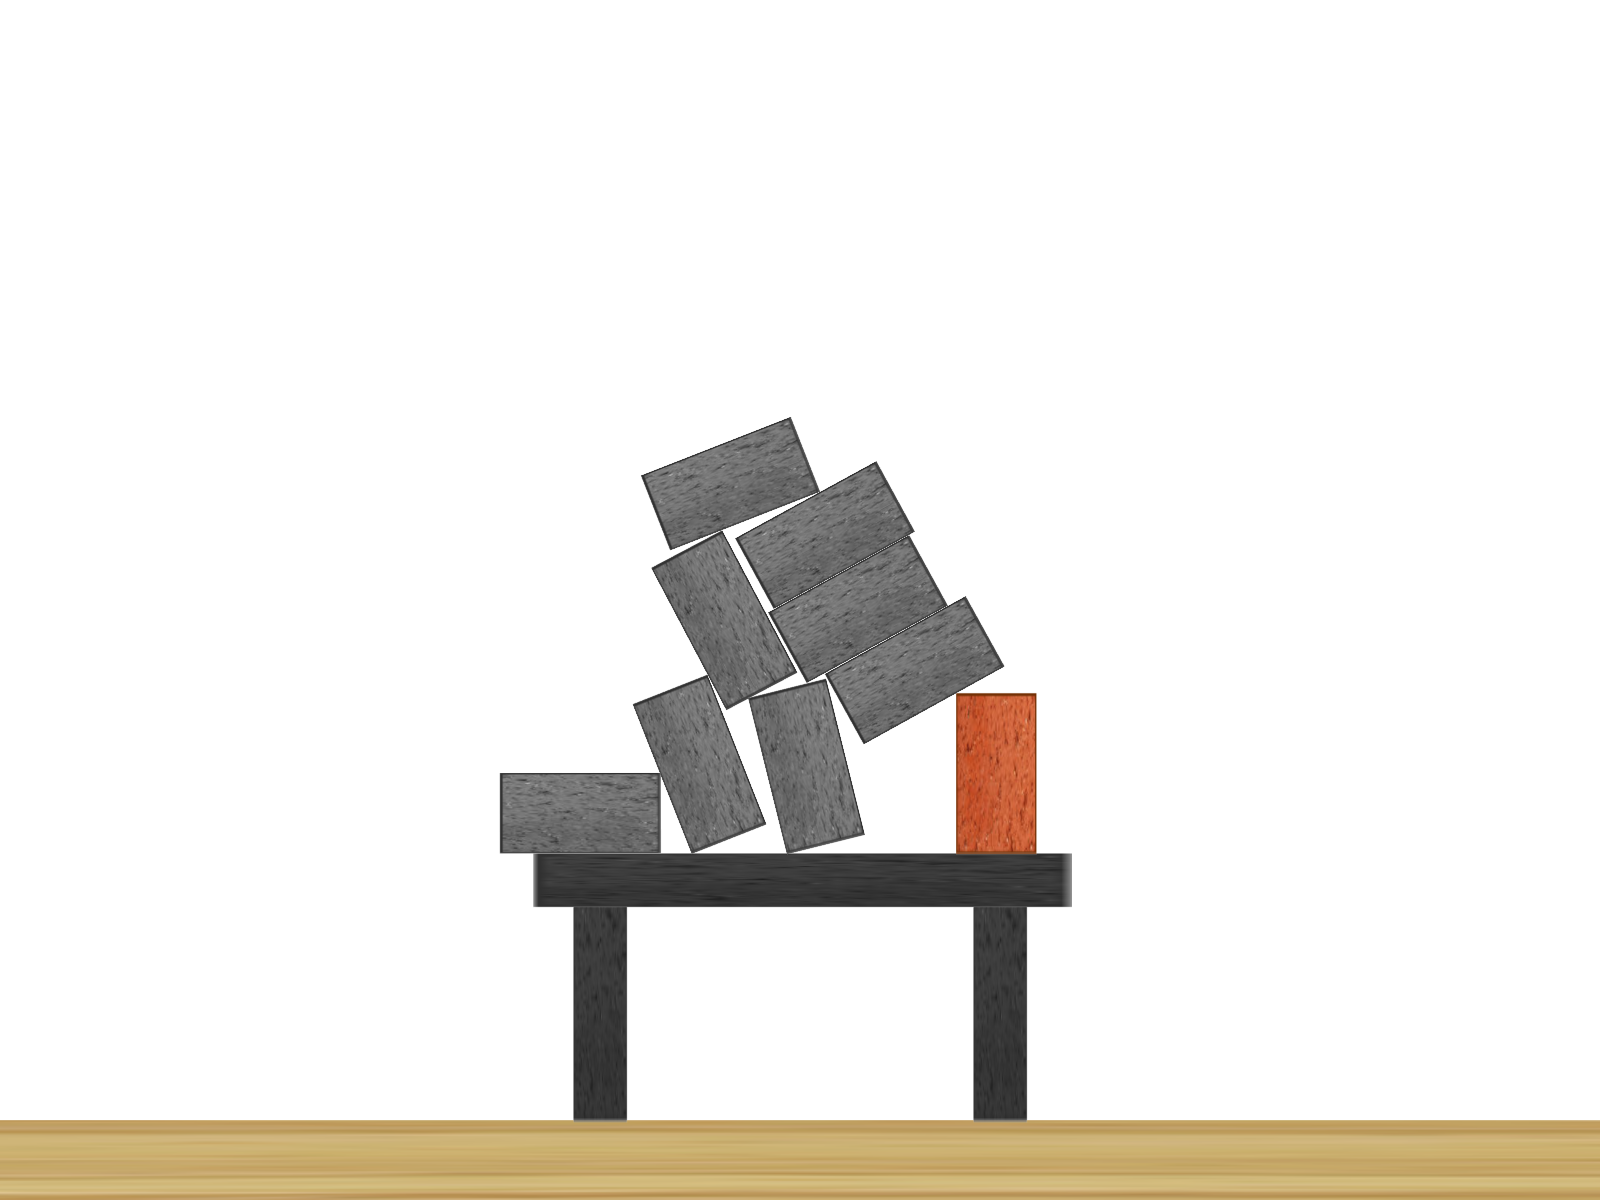
\includegraphics[width=0.2\columnwidth]{tower_image_(21)}}
% \hfill
% \subfloat[][bricks before: \textbf{8} (image~22)]{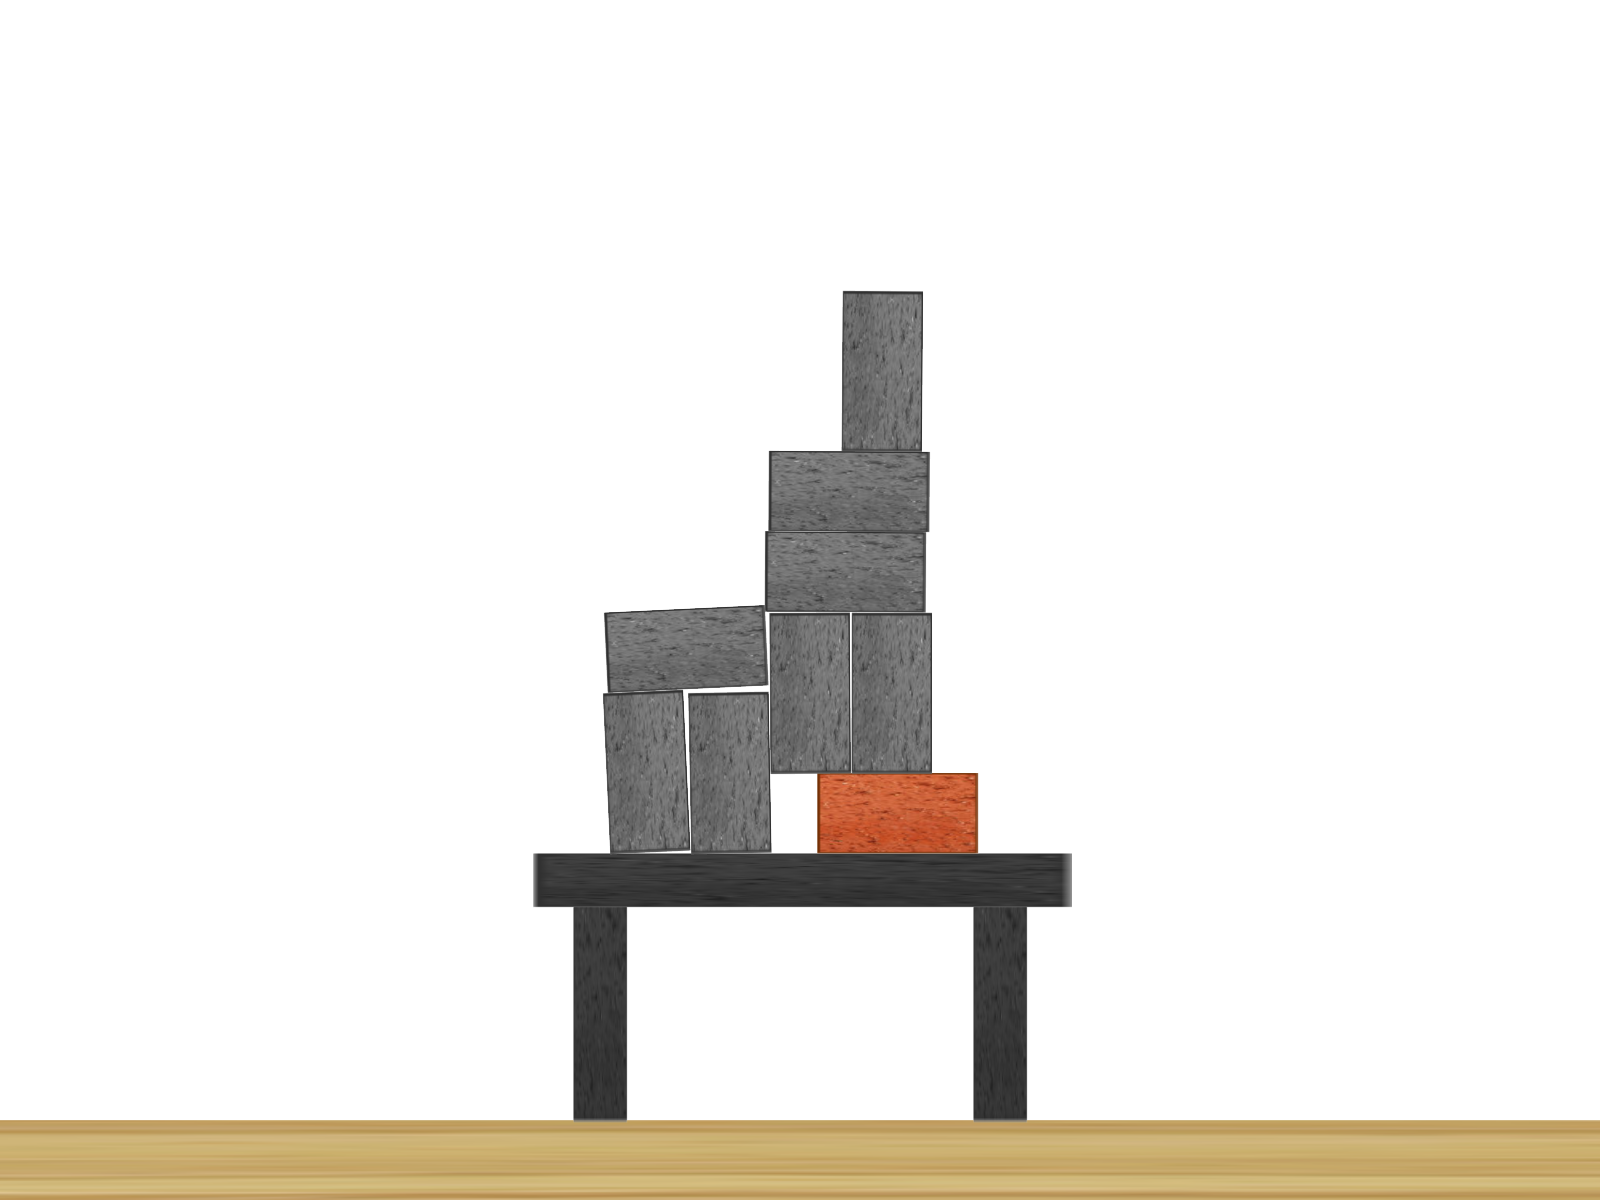
\includegraphics[width=0.2\columnwidth]{tower_image_(22)}}
% {\hfill}

% {\hfill}
% \subfloat[][bricks before: \textbf{5} (image~23)]{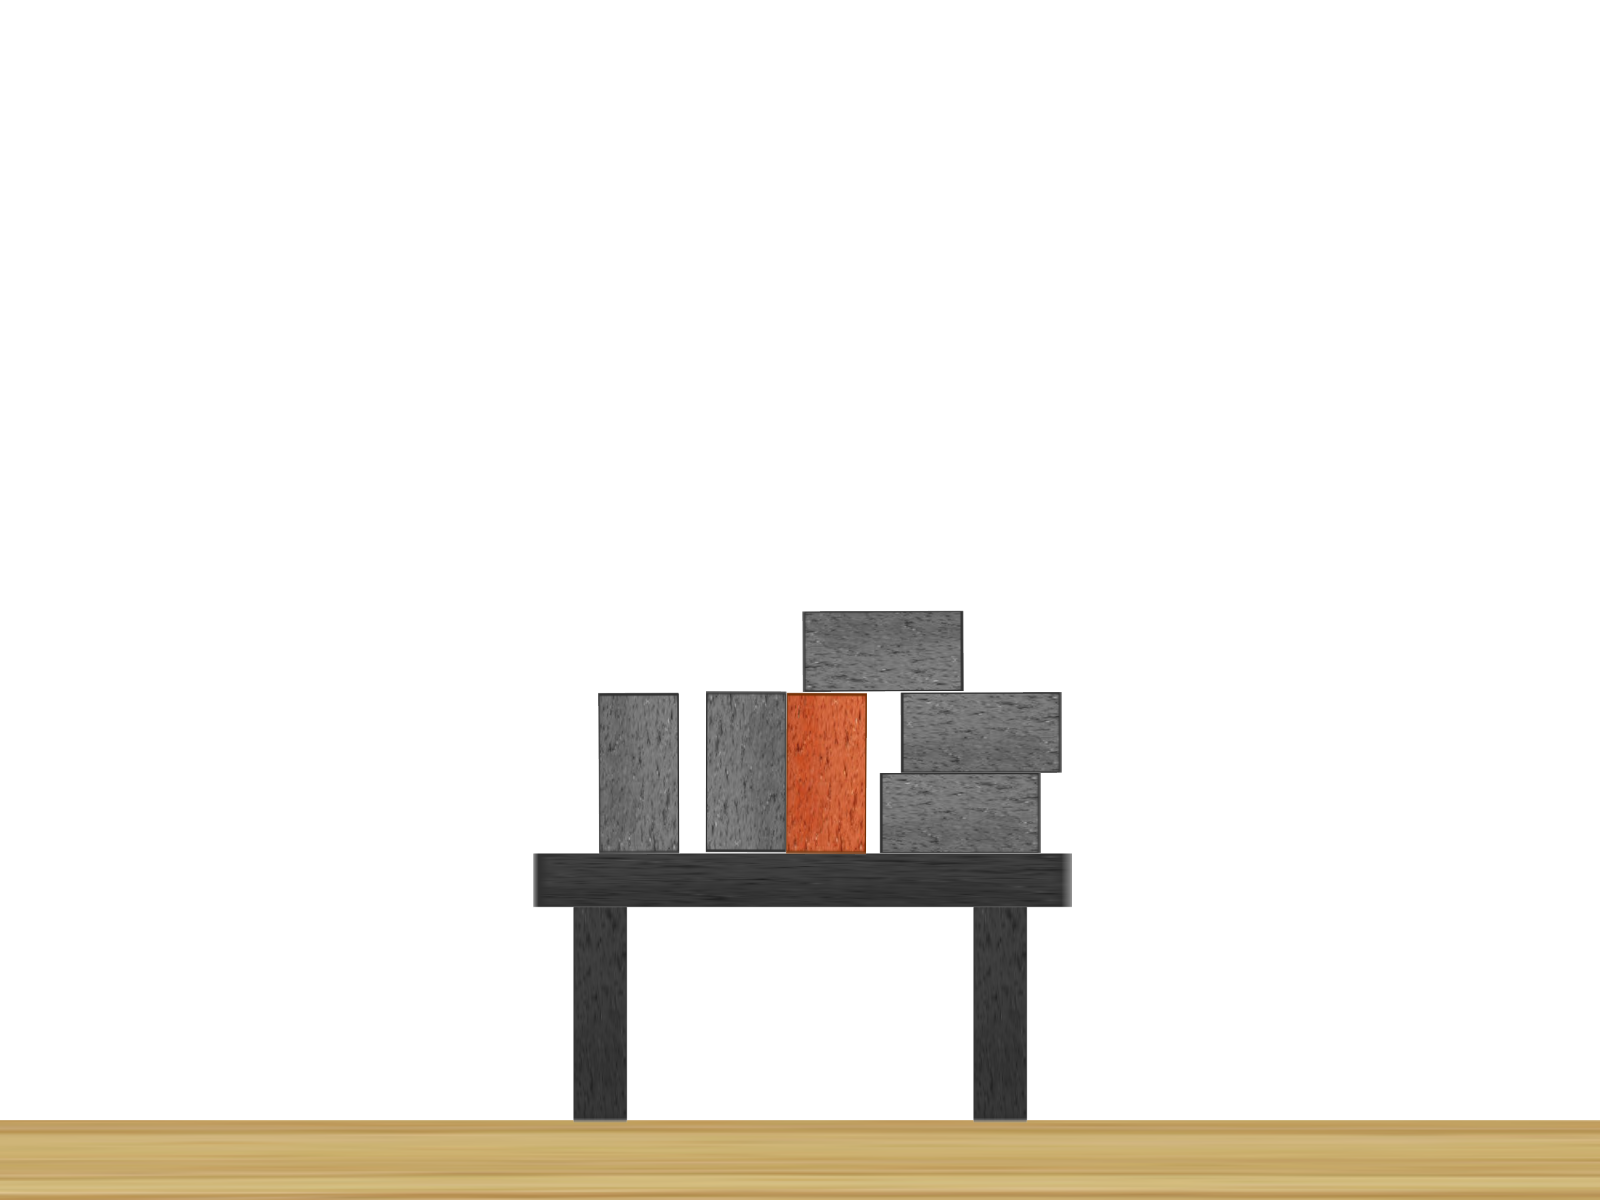
\includegraphics[width=0.2\columnwidth]{tower_image_(23)}}
% \hfill
% \subfloat[][bricks before: \textbf{5} (image~25)]{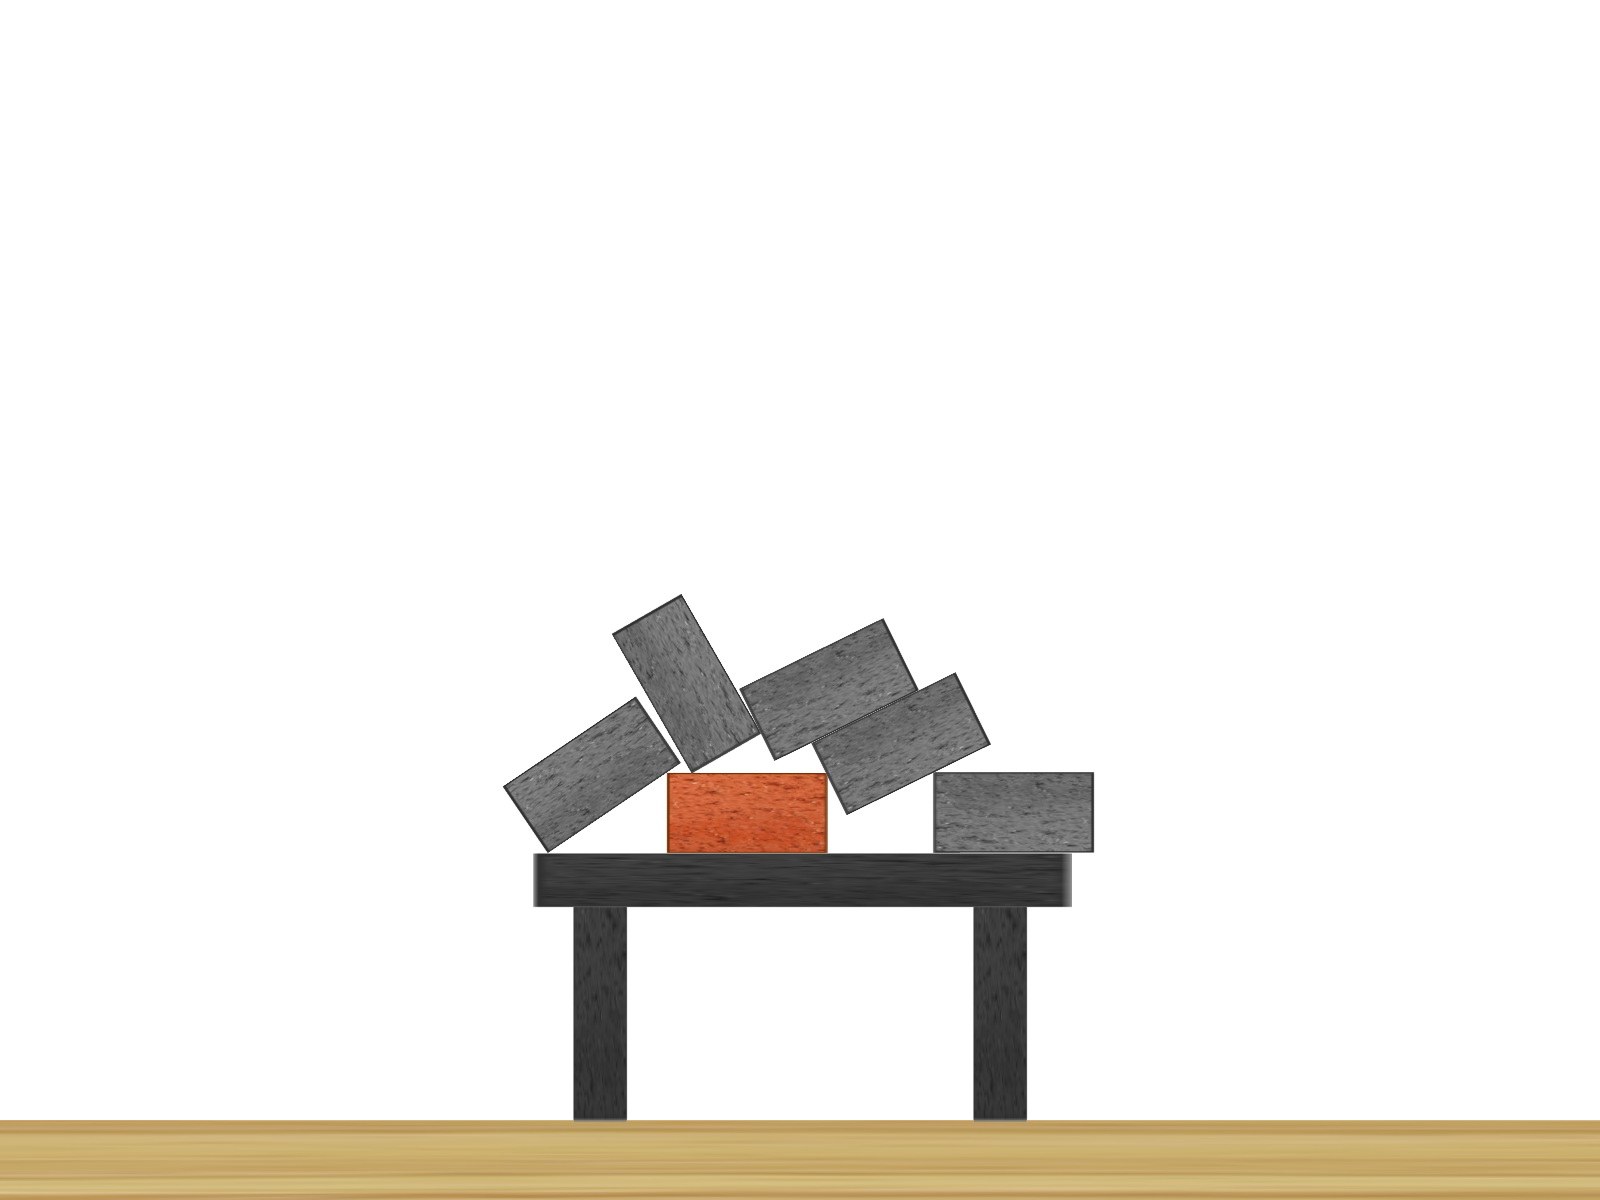
\includegraphics[width=0.2\columnwidth]{tower_image_(25)}}
% \hfill
% \subfloat[][bricks before: \textbf{12} (image~26)]{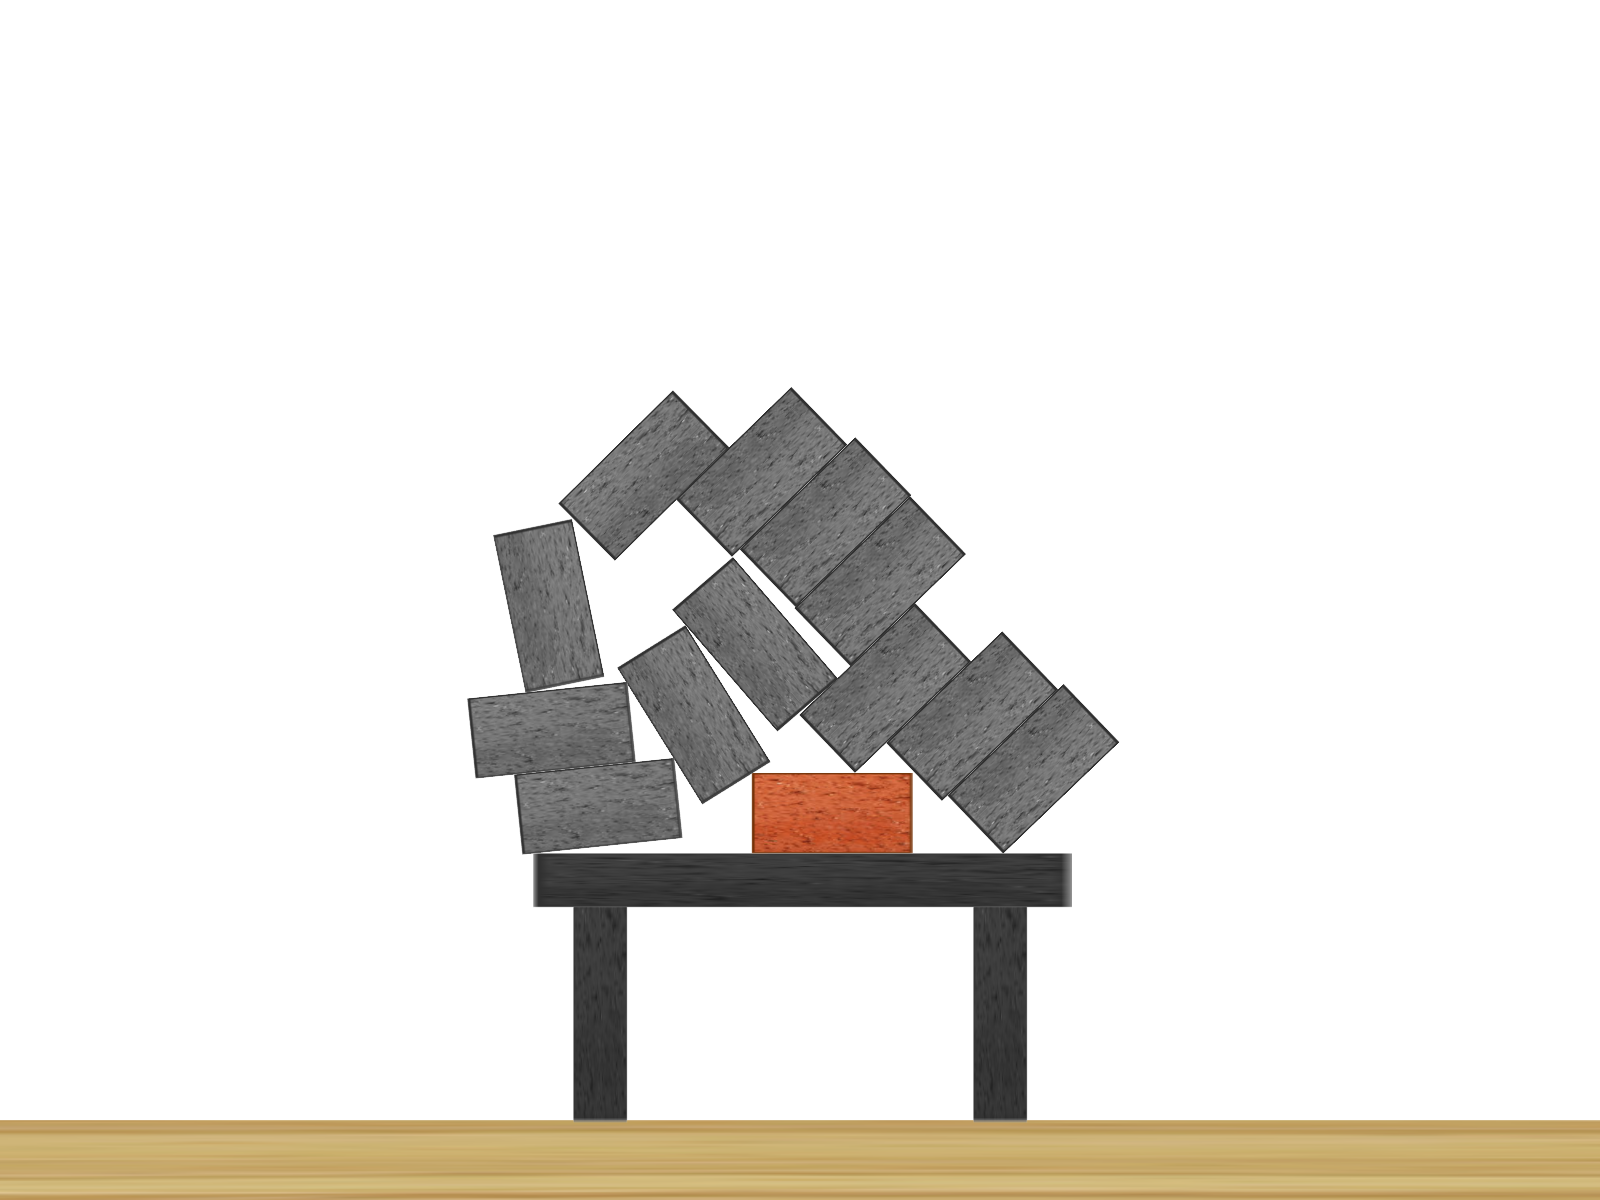
\includegraphics[width=0.2\columnwidth]{tower_image_(26)}}
% \hfill
% \subfloat[][bricks before: \textbf{10} (image~27)]{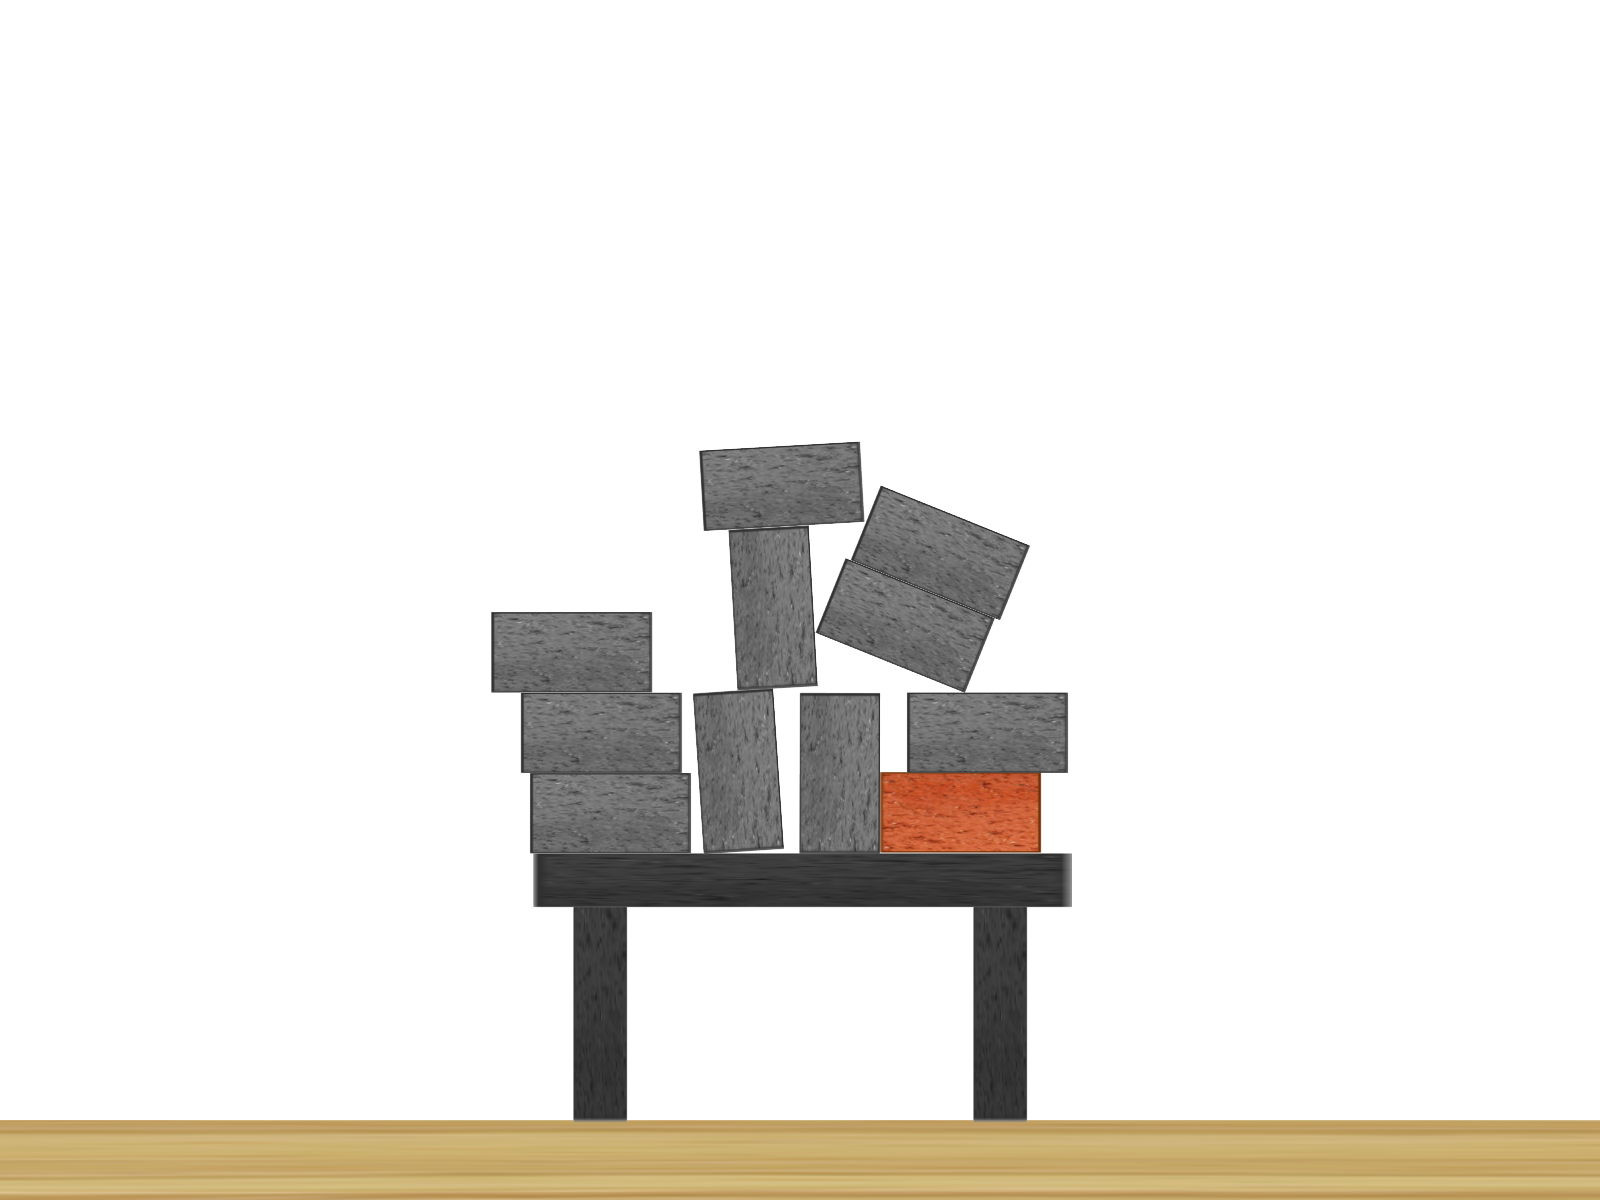
\includegraphics[width=0.2\columnwidth]{tower_image_(27)}}
% {\hfill}
% % \caption{Stimuli.}
% \end{figure}

% \clearpage

% \begin{figure}[H]
% % \ContinuedFloat
% \renewcommand{\thesubfigure}{\arabic{subfigure}}
%  % \addtocounter{subfigure}{20} 
% {\hfill}
% \subfloat[][bricks before: \textbf{7} (image~28)]{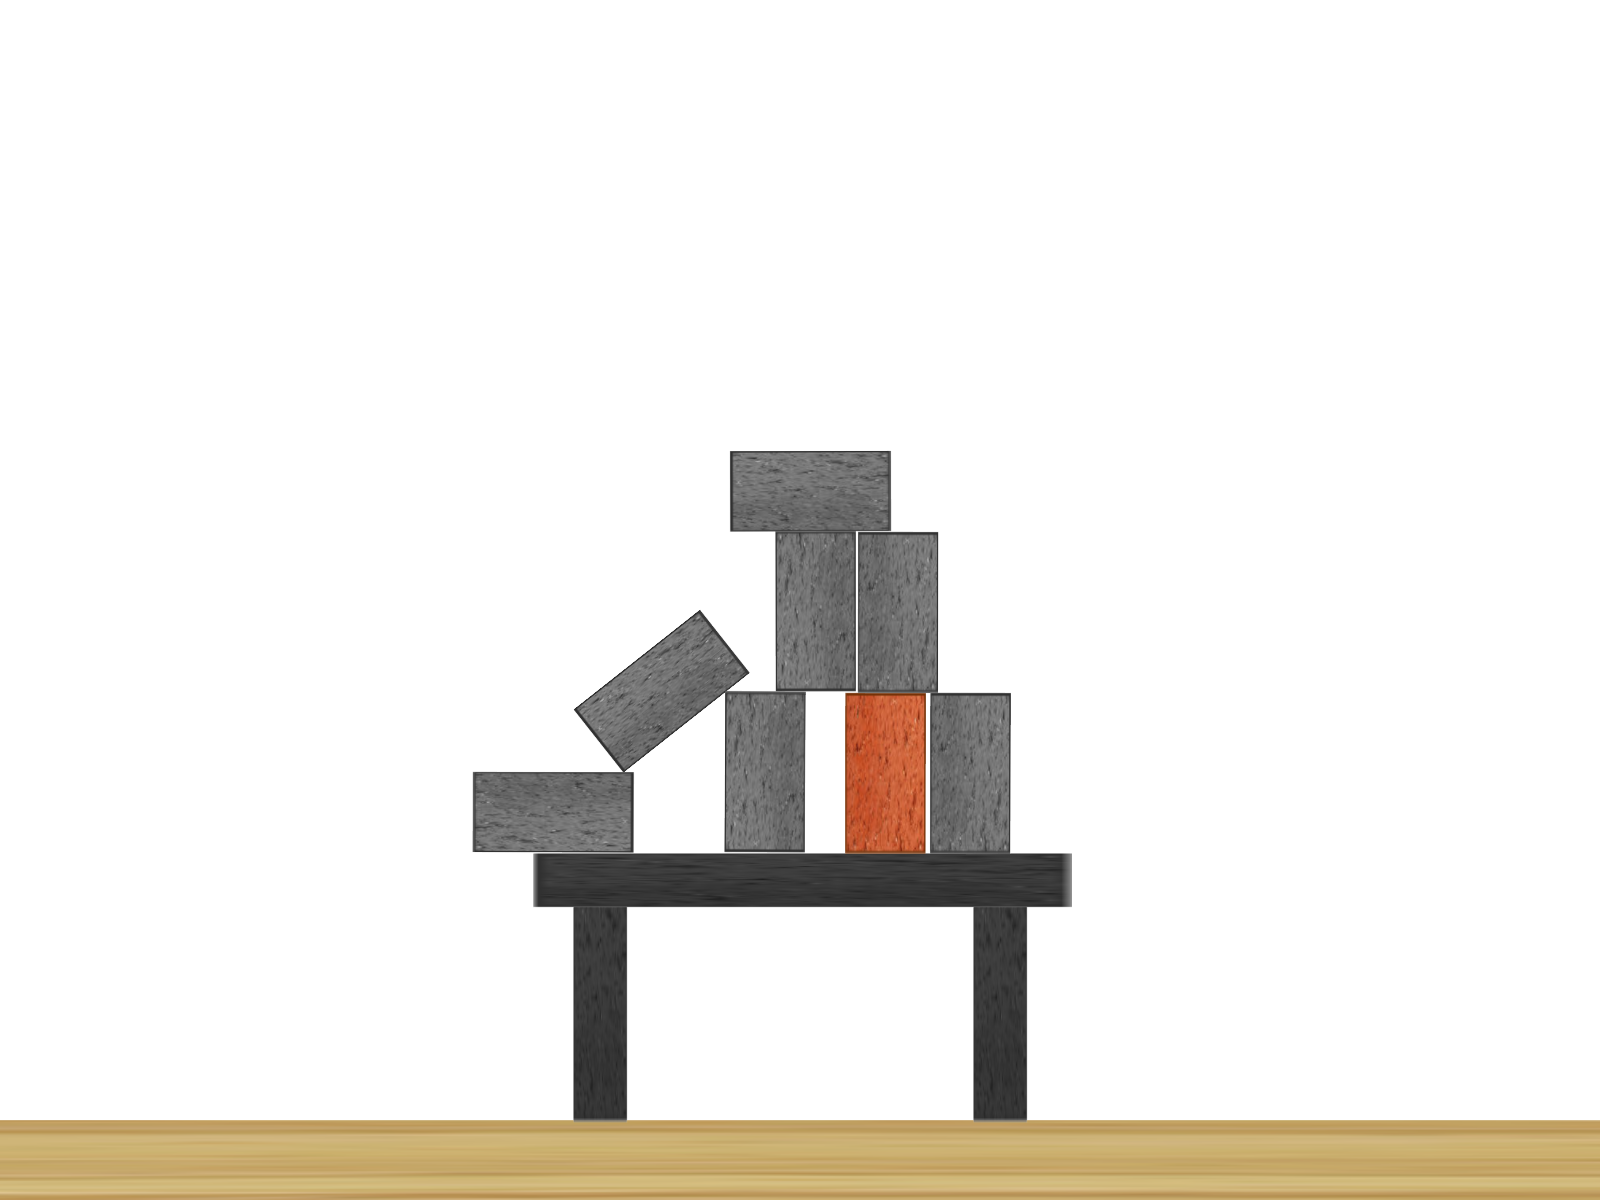
\includegraphics[width=0.2\columnwidth]{tower_image_(28)}}
% \hfill
% \subfloat[][bricks before: \textbf{5} (image~29)]{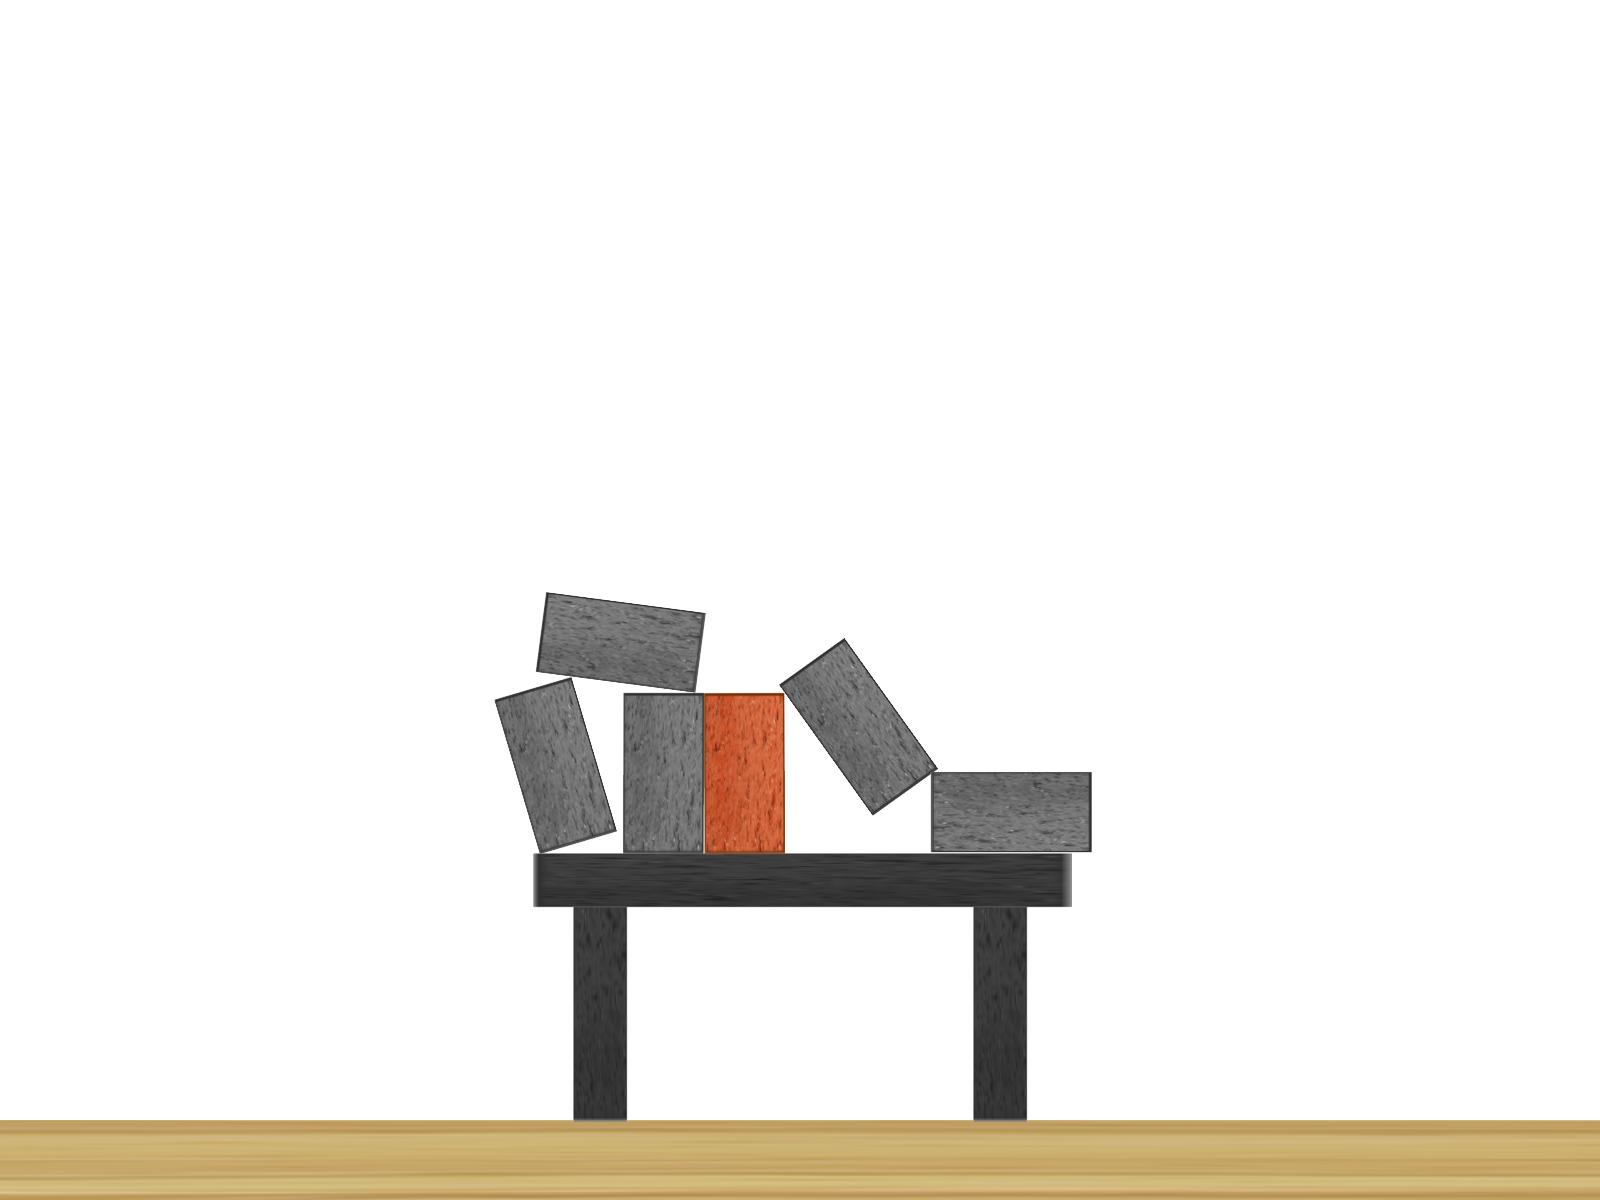
\includegraphics[width=0.2\columnwidth]{tower_image_(29)}}
% \hfill
% \subfloat[][bricks before: \textbf{9} (image~30)]{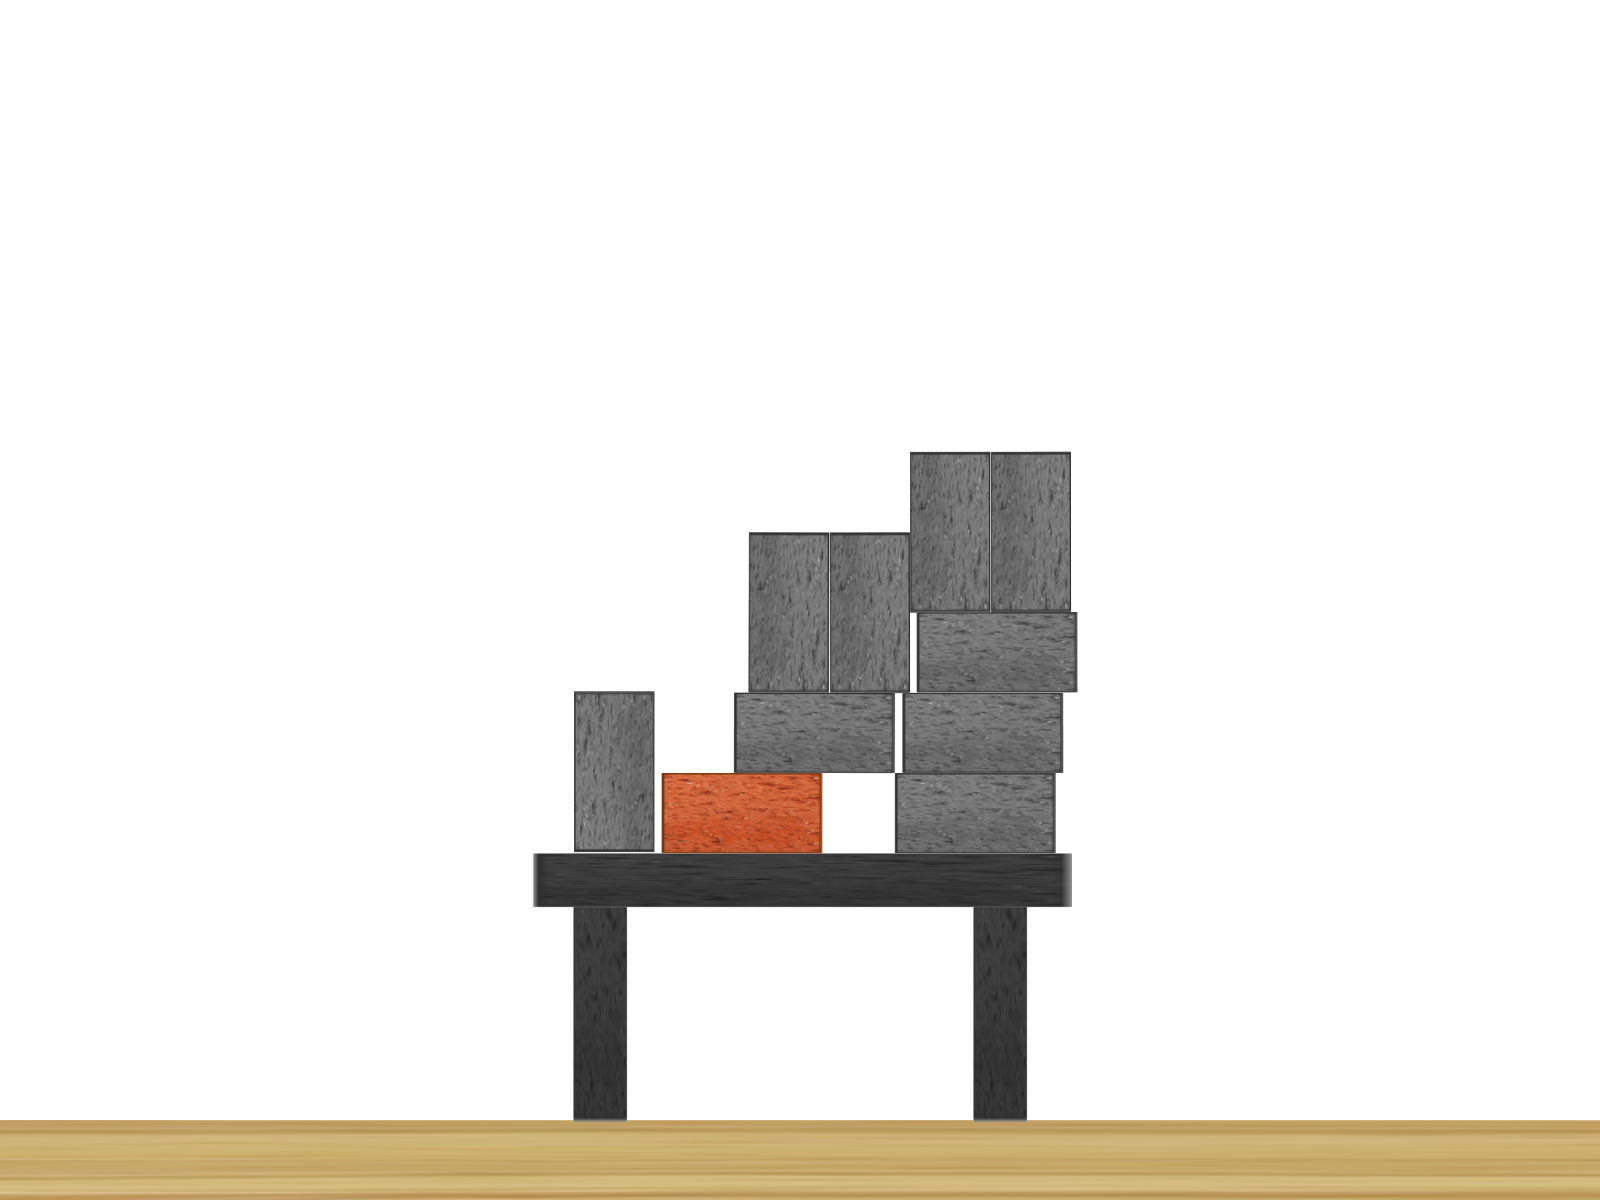
\includegraphics[width=0.2\columnwidth]{tower_image_(30)}}
% \hfill
% \subfloat[][bricks before: \textbf{13} (image~31)]{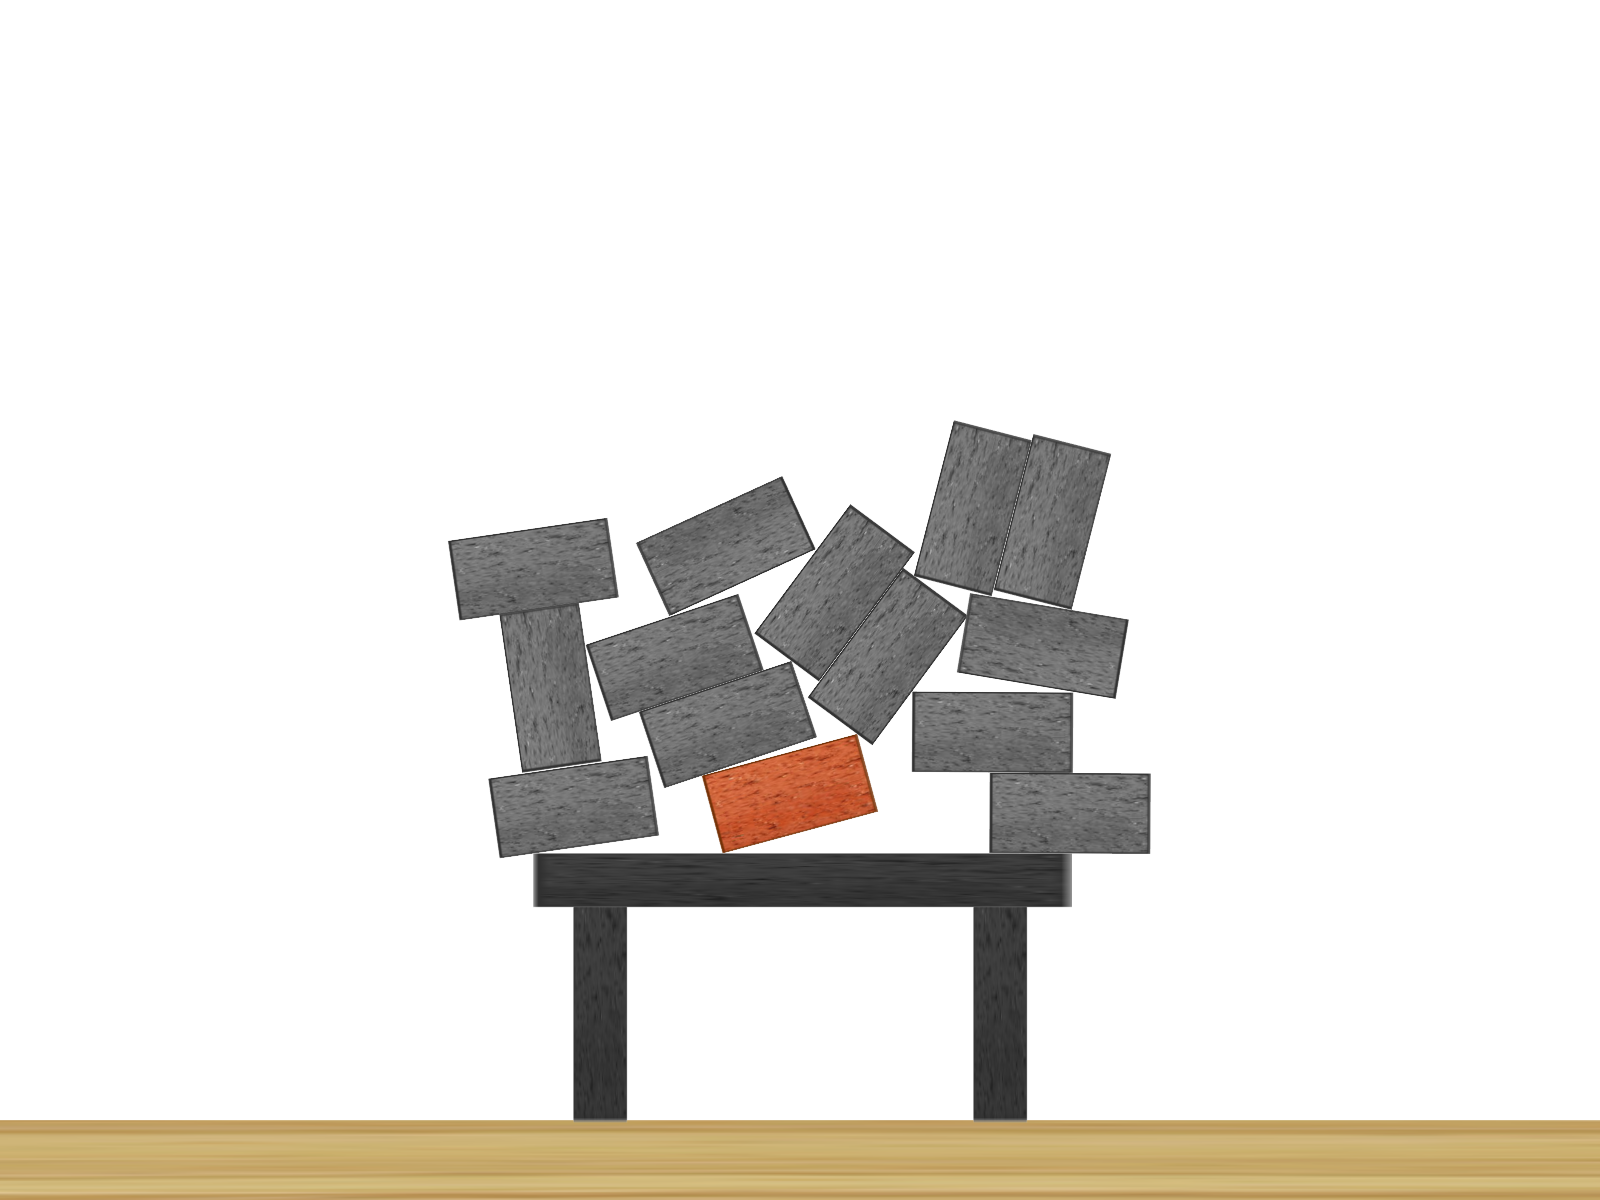
\includegraphics[width=0.2\columnwidth]{tower_image_(31)}}
% {\hfill}

% {\hfill}
% \subfloat[][bricks before: \textbf{4} (image~32)]{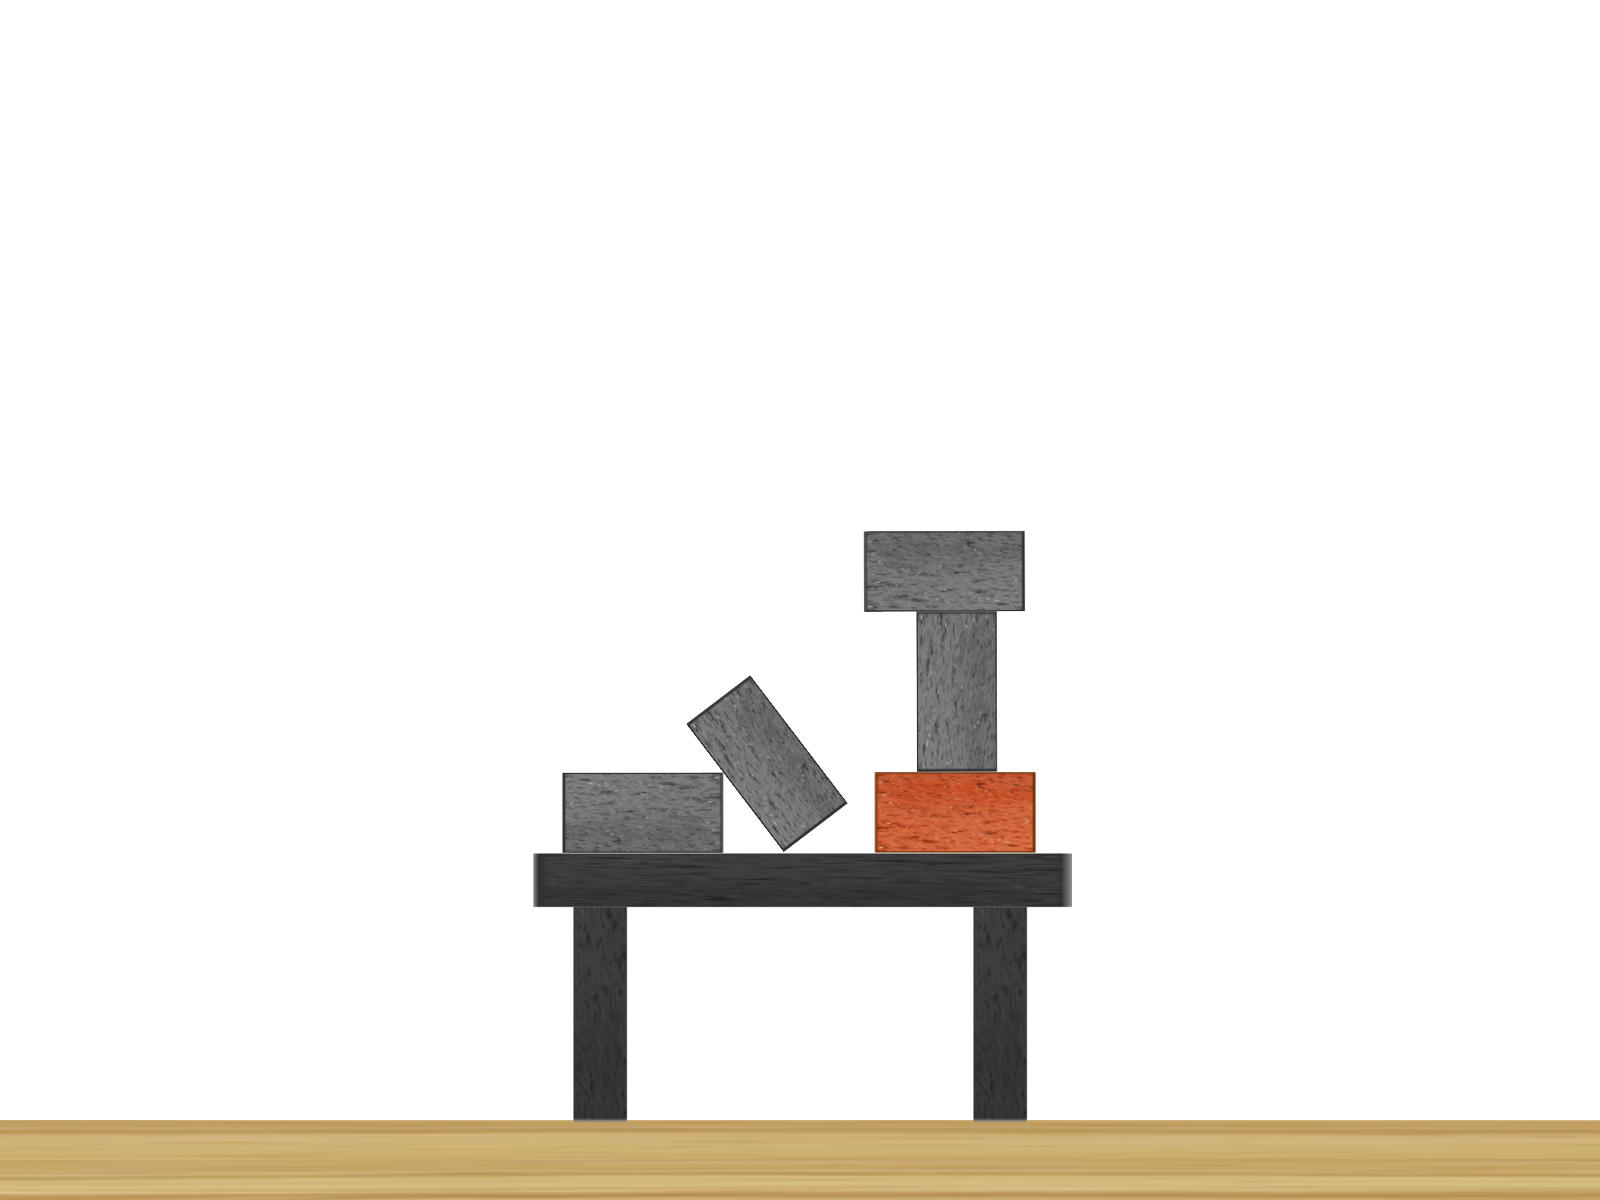
\includegraphics[width=0.2\columnwidth]{tower_image_(32)}}
% \hfill
% \subfloat[][bricks before: \textbf{6} (image~33)]{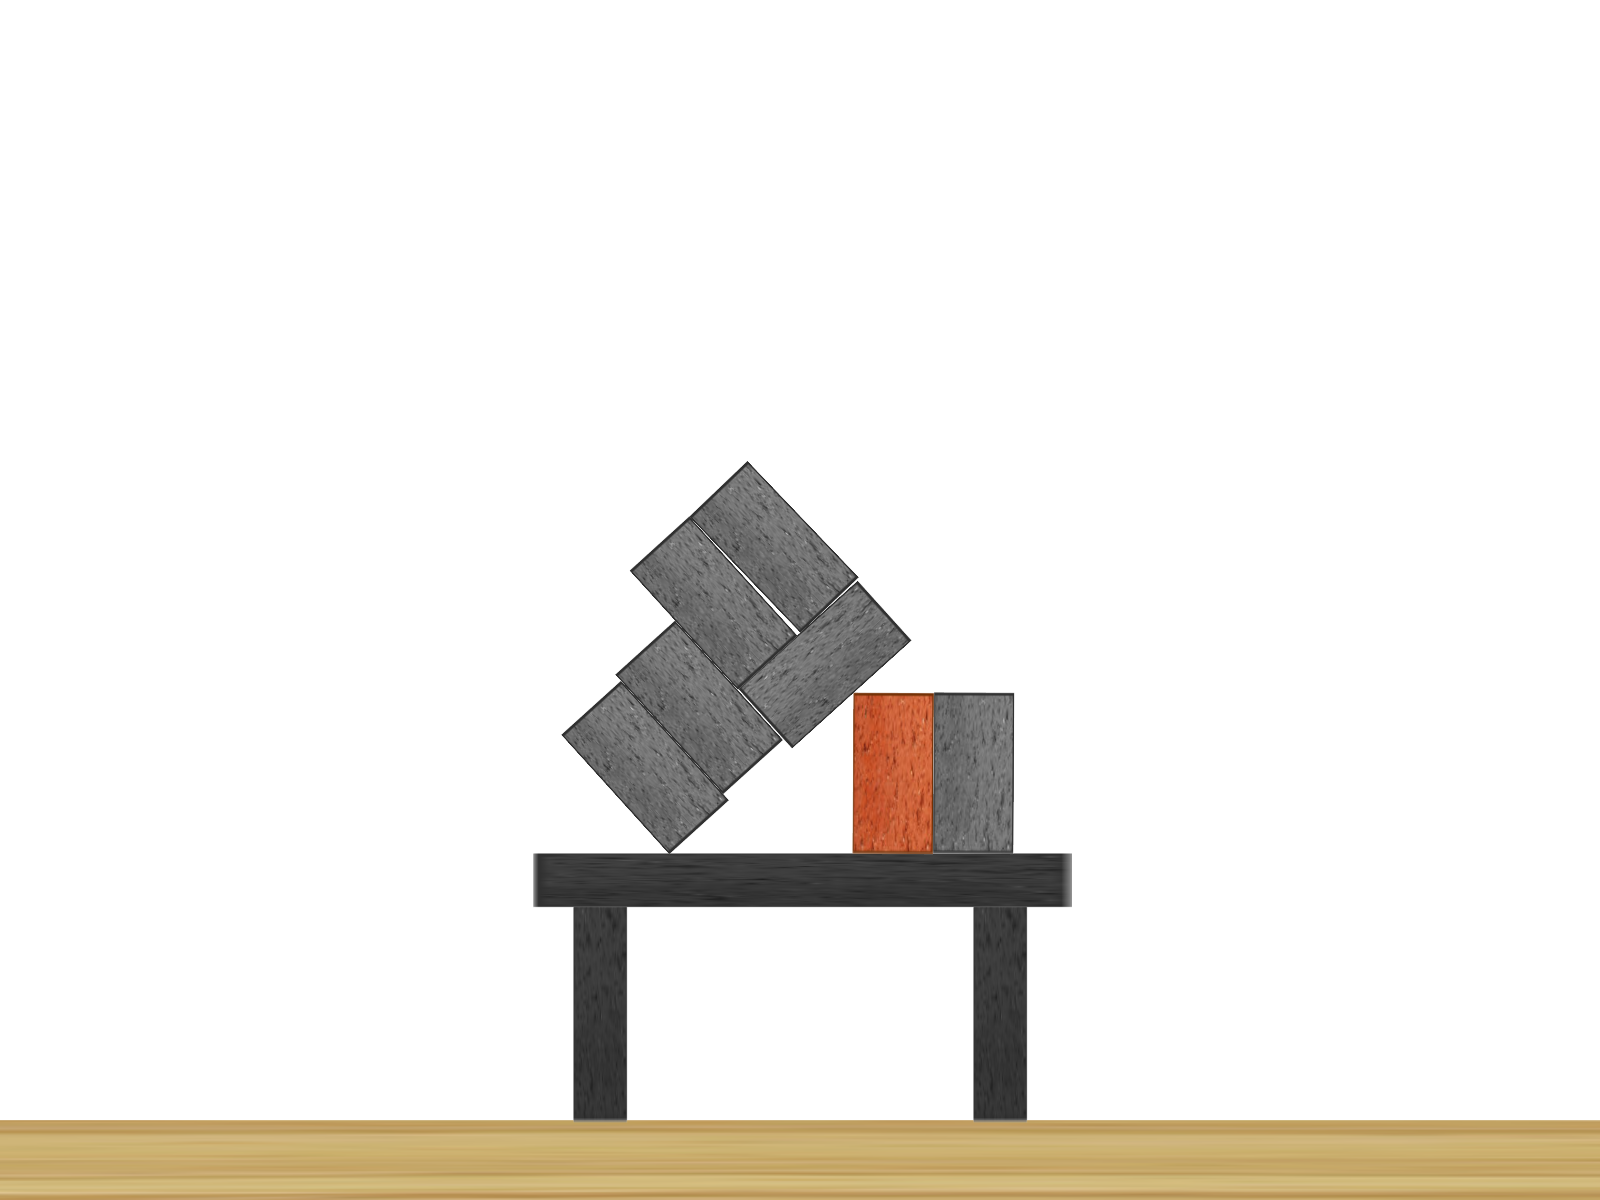
\includegraphics[width=0.2\columnwidth]{tower_image_(33)}}
% \hfill
% \subfloat[][bricks before: \textbf{5} (image~34)]{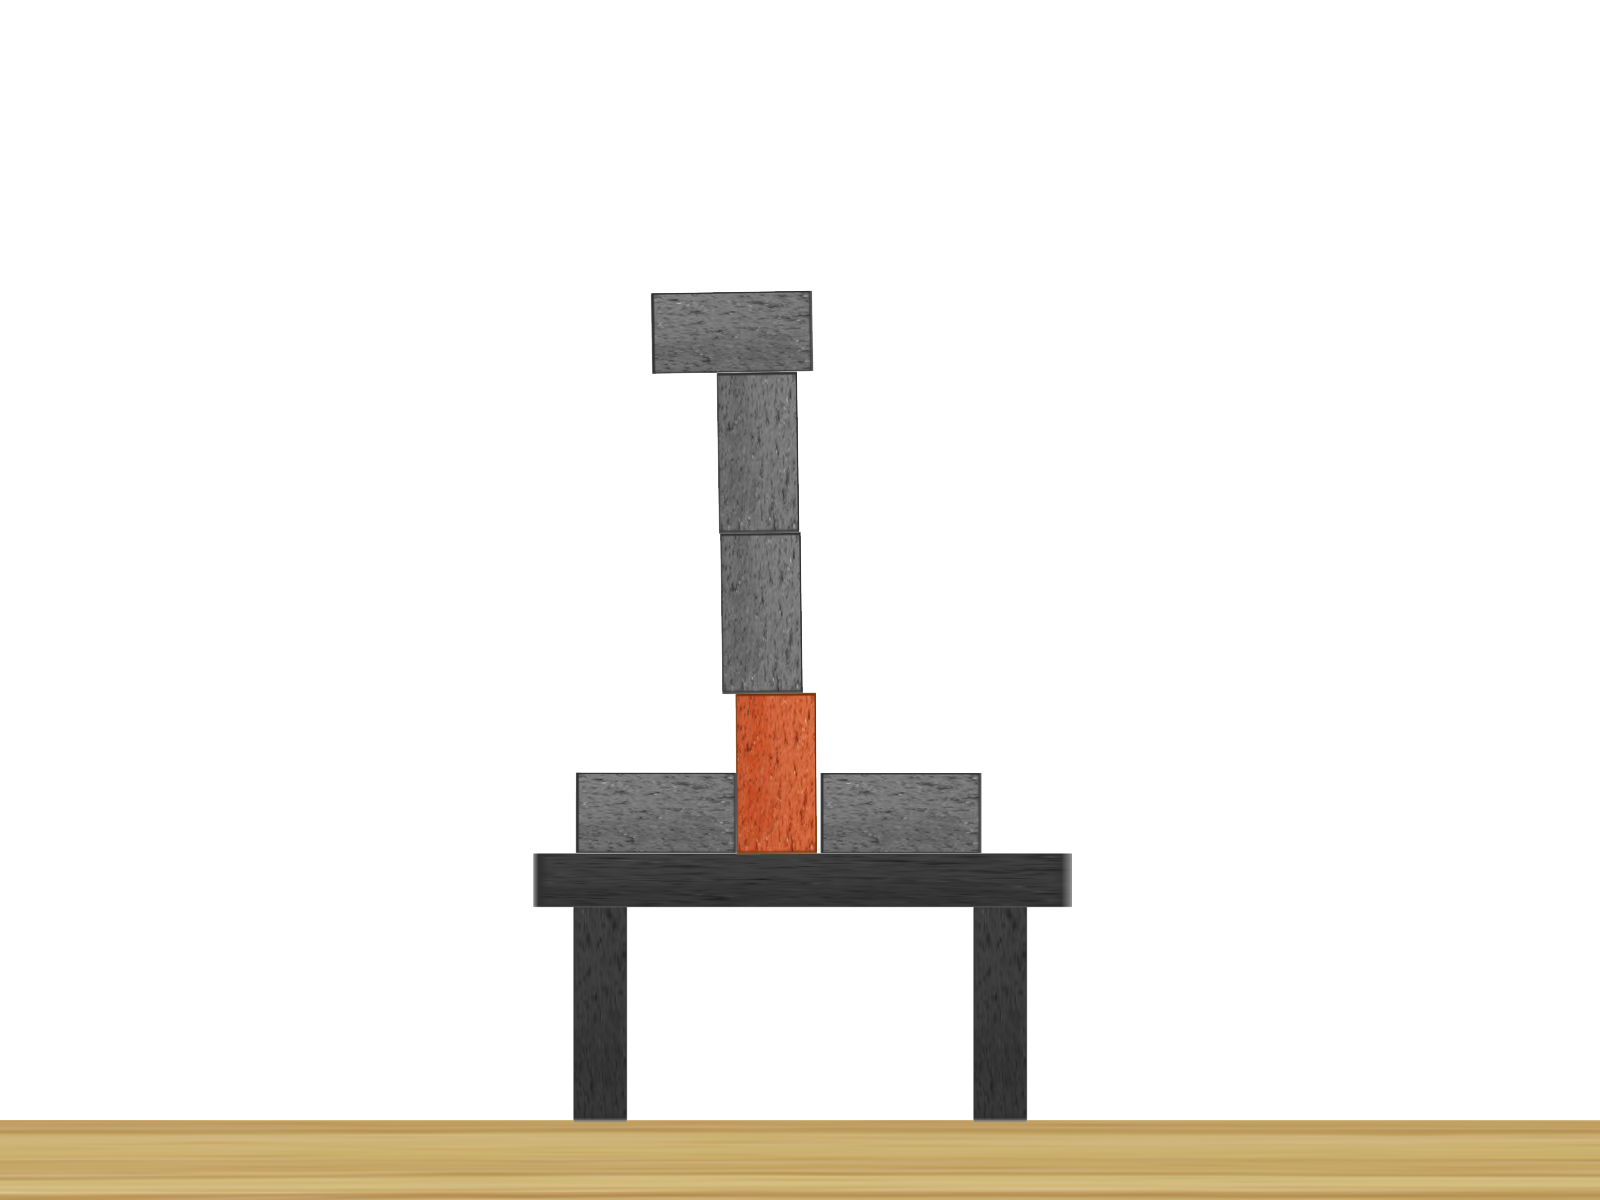
\includegraphics[width=0.2\columnwidth]{tower_image_(34)}}
% \hfill
% \subfloat[][bricks before: \textbf{5} (image~35)]{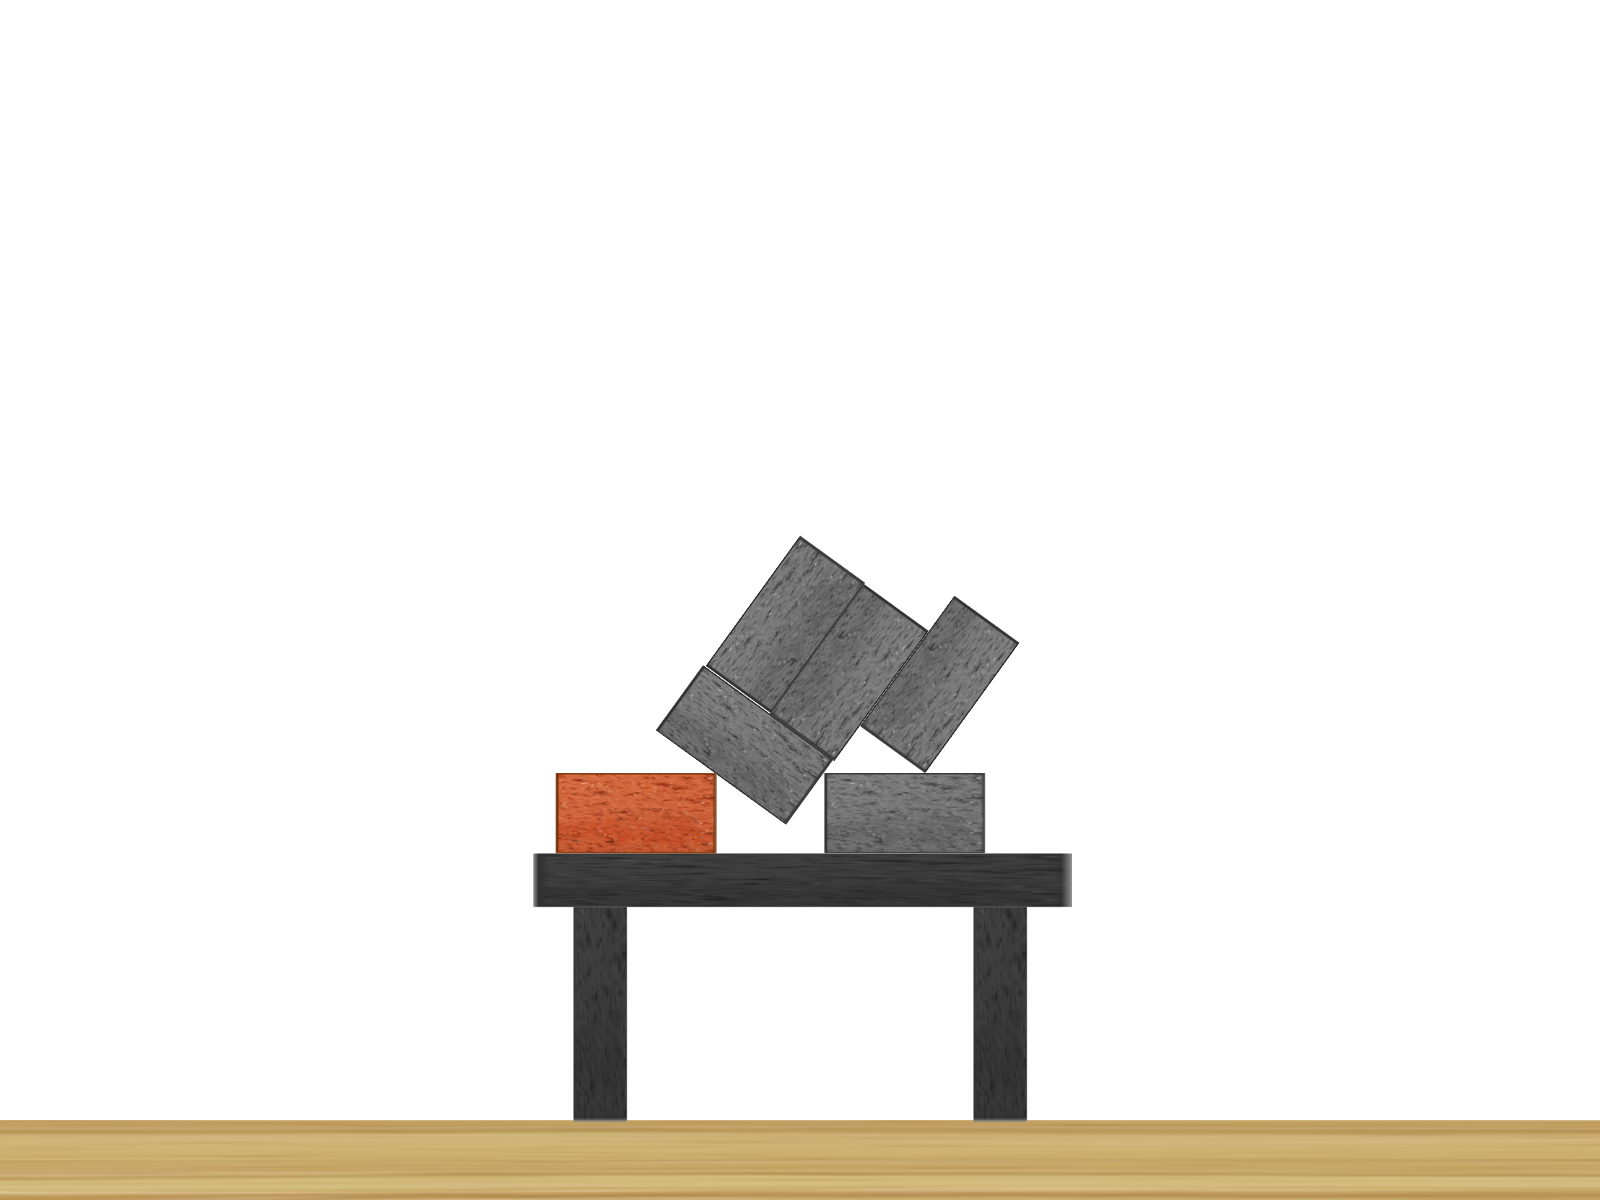
\includegraphics[width=0.2\columnwidth]{tower_image_(35)}}
% {\hfill}

% {\hfill}
% \subfloat[][bricks before: \textbf{6} (image~36)]{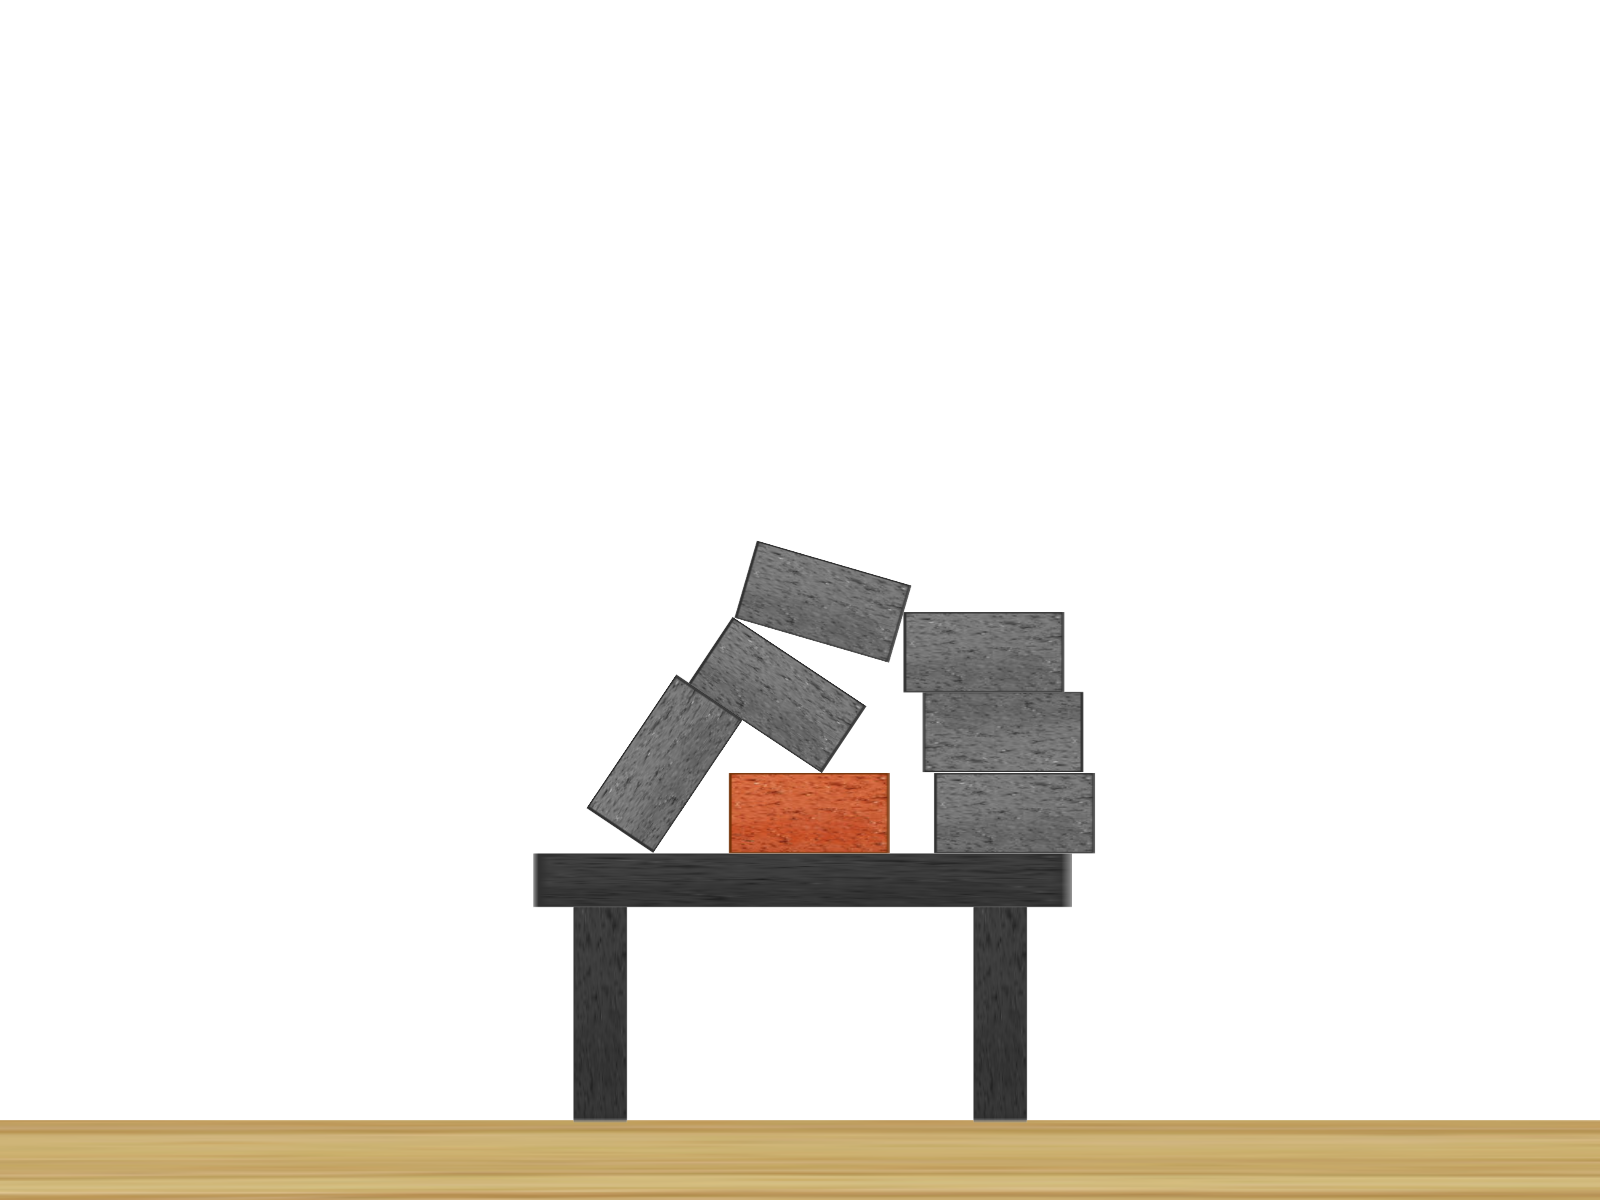
\includegraphics[width=0.2\columnwidth]{tower_image_(36)}}
% \hfill
% \subfloat[][bricks before: \textbf{10} (image~37)]{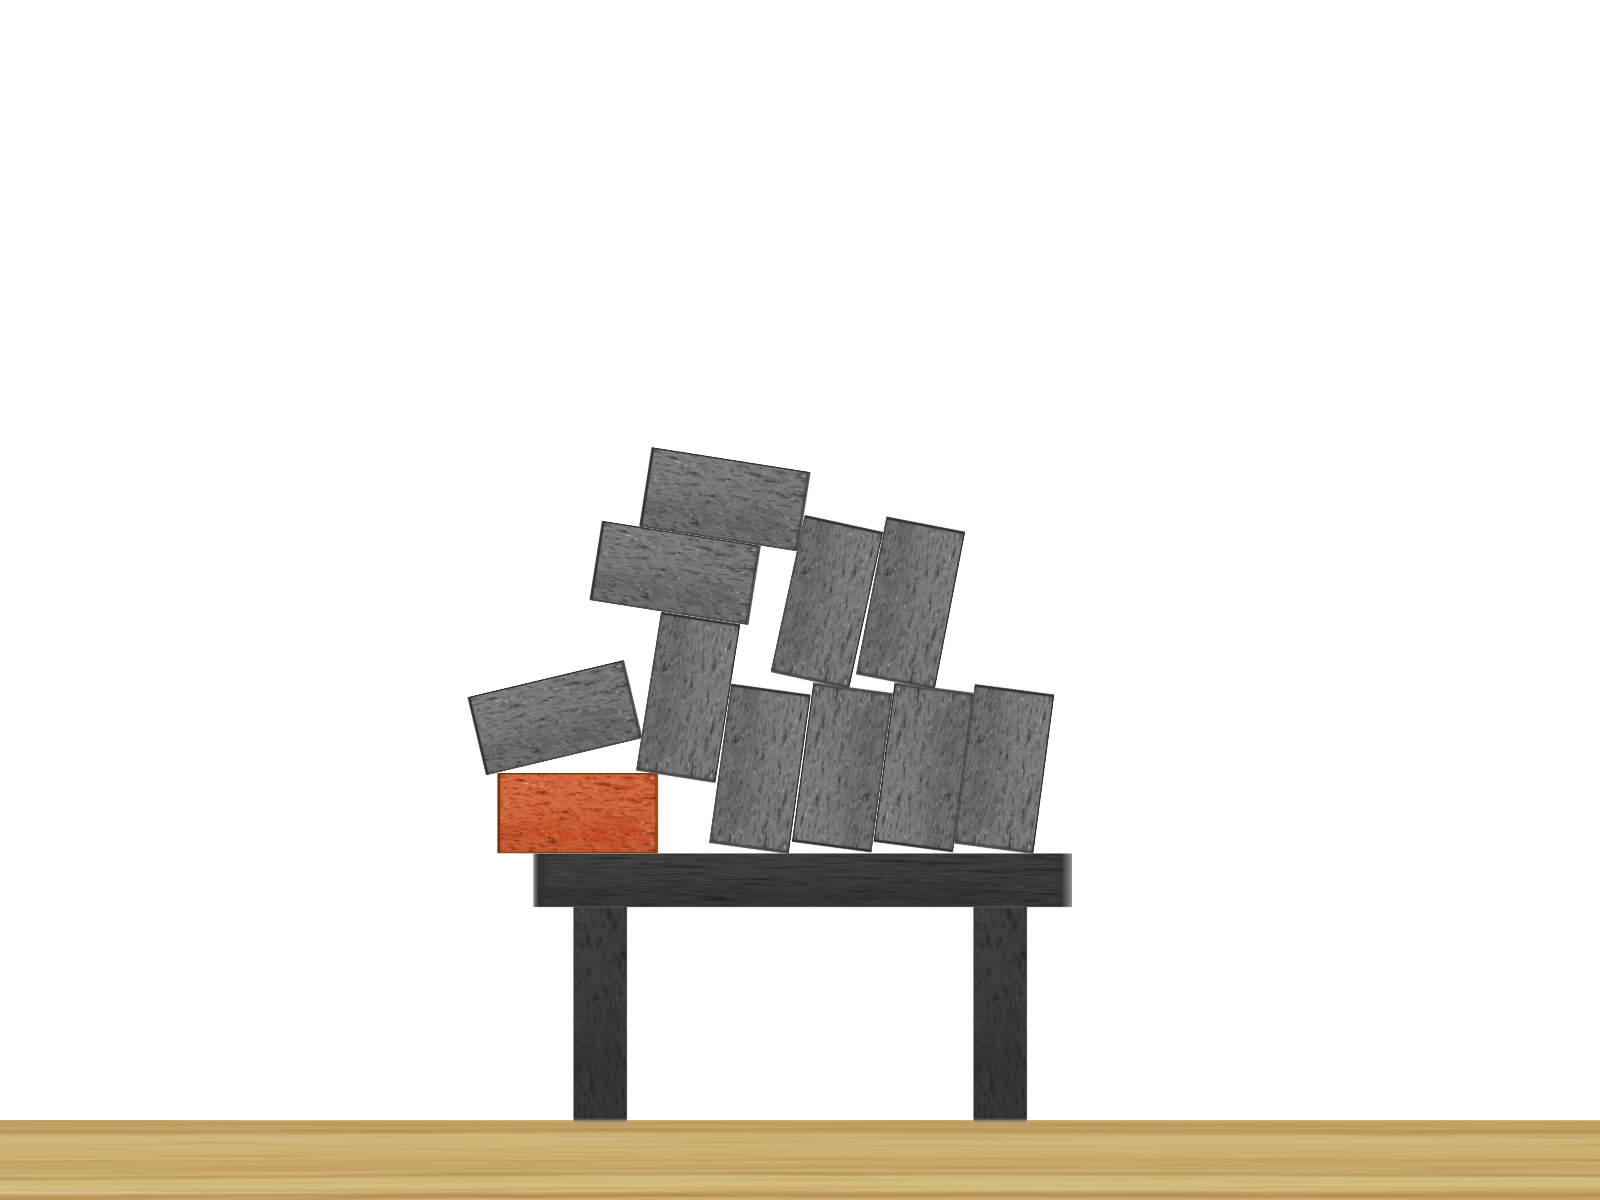
\includegraphics[width=0.2\columnwidth]{tower_image_(37)}}
% {\hfill}
% \caption{Stimuli}
% \label{fig:Stimuli}
% \end{figure}

% \subsection{Model}
% \label{sub:model}

% \subsubsection{Ground truth}
% \label{ssub:ground_truth}

% The \textbf{ground truth model} simply removes the red brick from the scene and notes how many bricks remained on the table. (I have tried out some noisy version of the model but haven't looked at it systematically yet.)

% The model records (1) how many blocks fell off the table, and (2) how many blocks changed their position (see Figure~\ref{fig:stimuli_after}).

% \begin{figure}[H]
% % \captionsetup[subfigure]{labelformat=empty}
% \renewcommand{\thesubfigure}{\arabic{subfigure}}
% \centering
% {\hfill}
% \subfloat[][fell \textbf{4}, changed \textbf{8}]{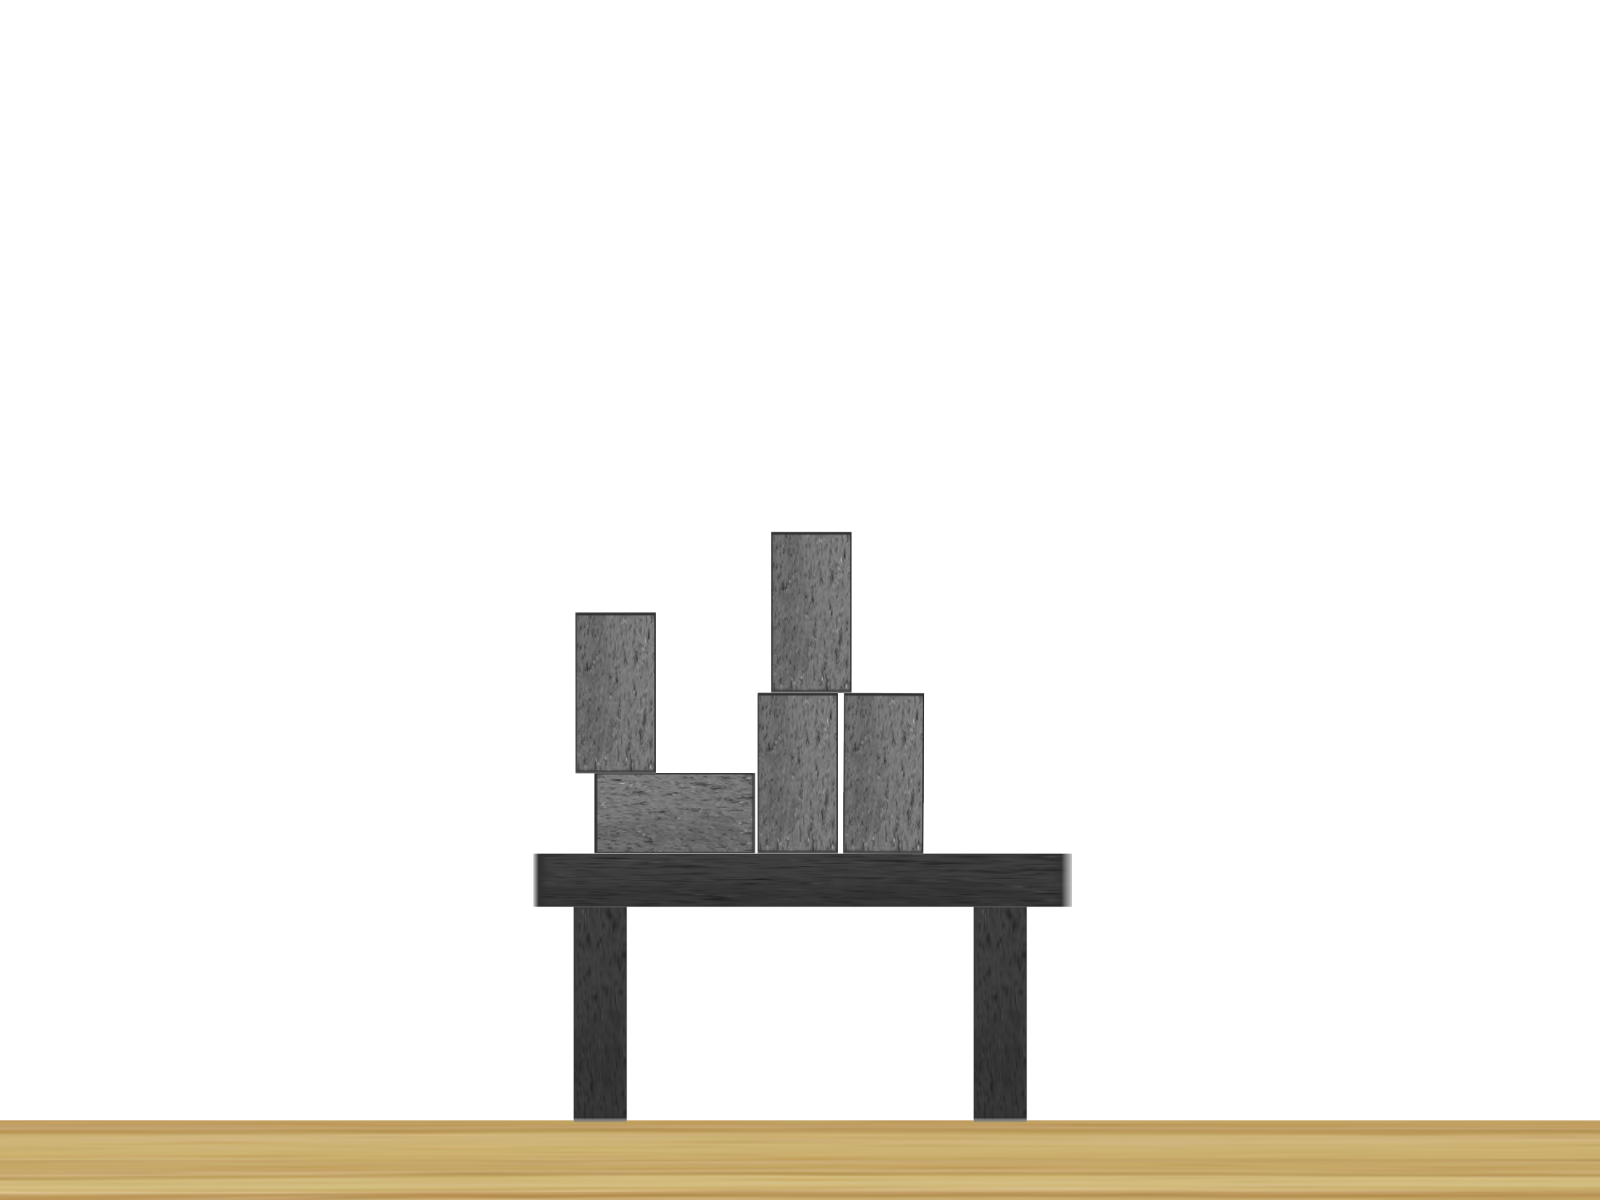
\includegraphics[width=0.2\columnwidth]{tower_image_after_(1)}}
% \hfill
% \subfloat[][fell \textbf{0}, changed \textbf{7}]{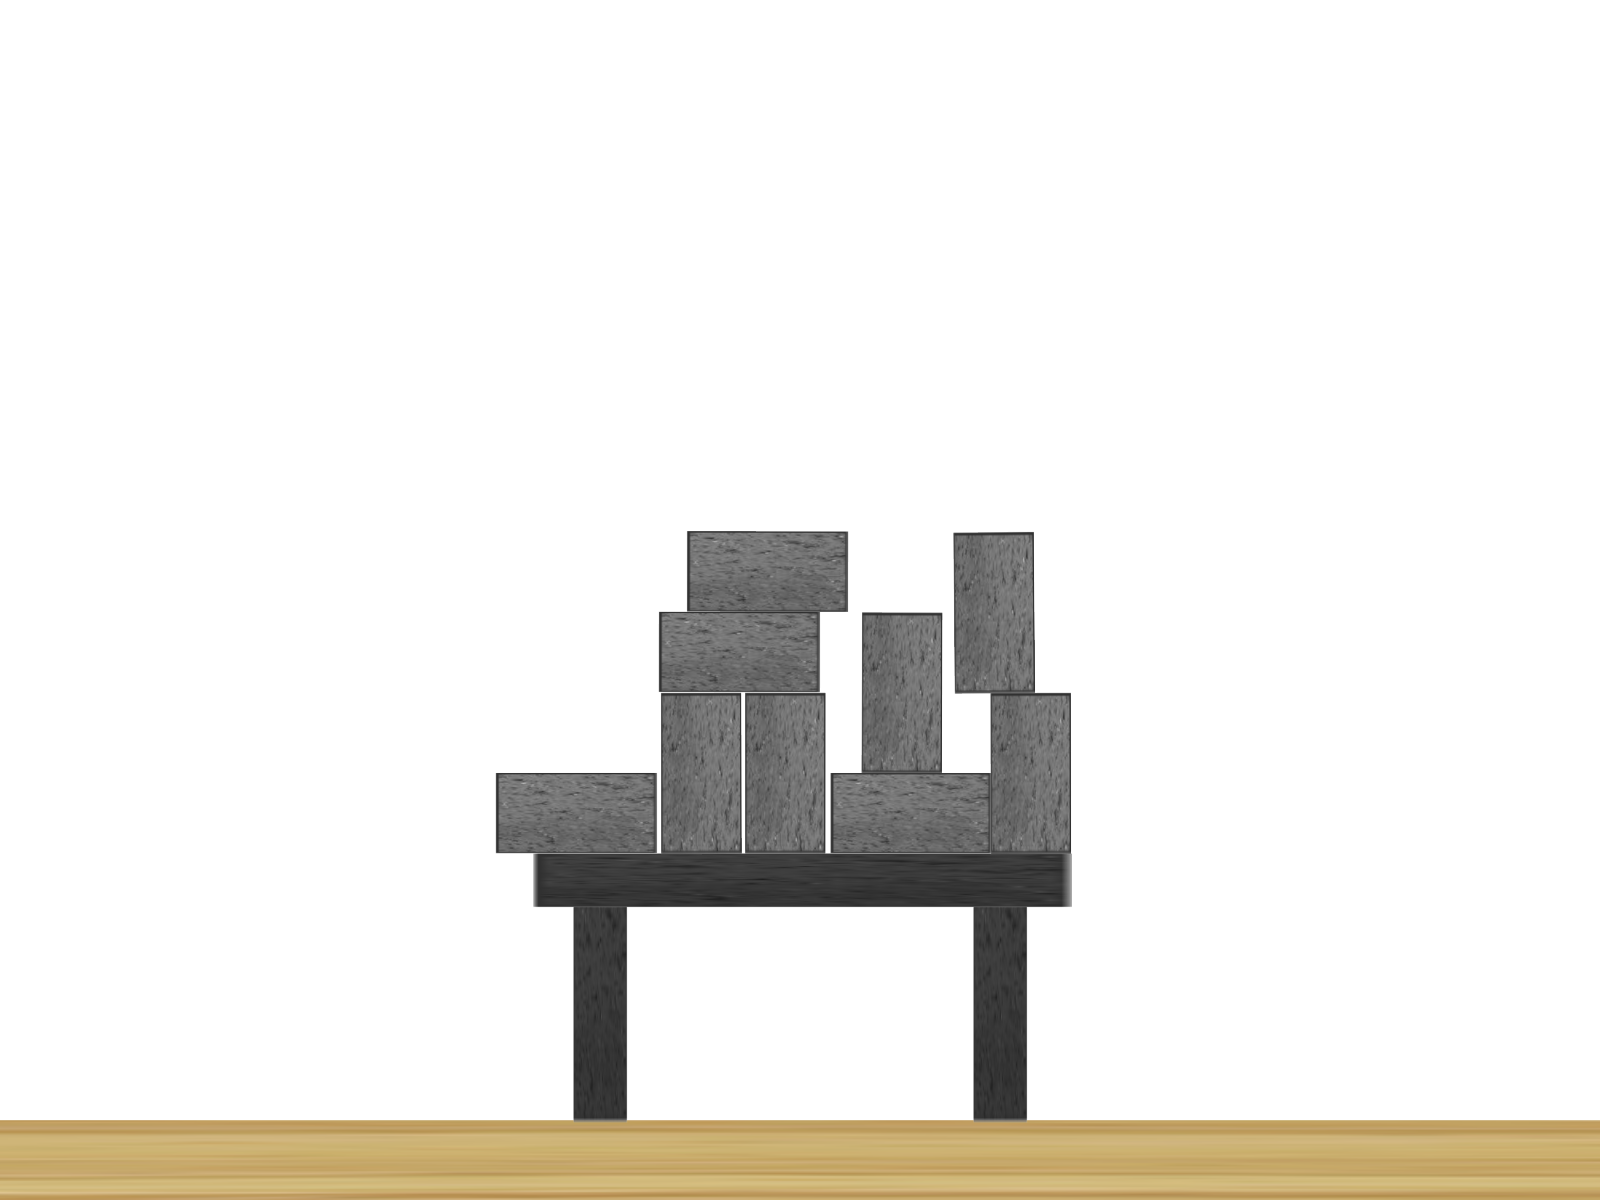
\includegraphics[width=0.2\columnwidth]{tower_image_after_(2)}}
% \hfill
% \subfloat[][fell \textbf{7}, changed \textbf{14}]{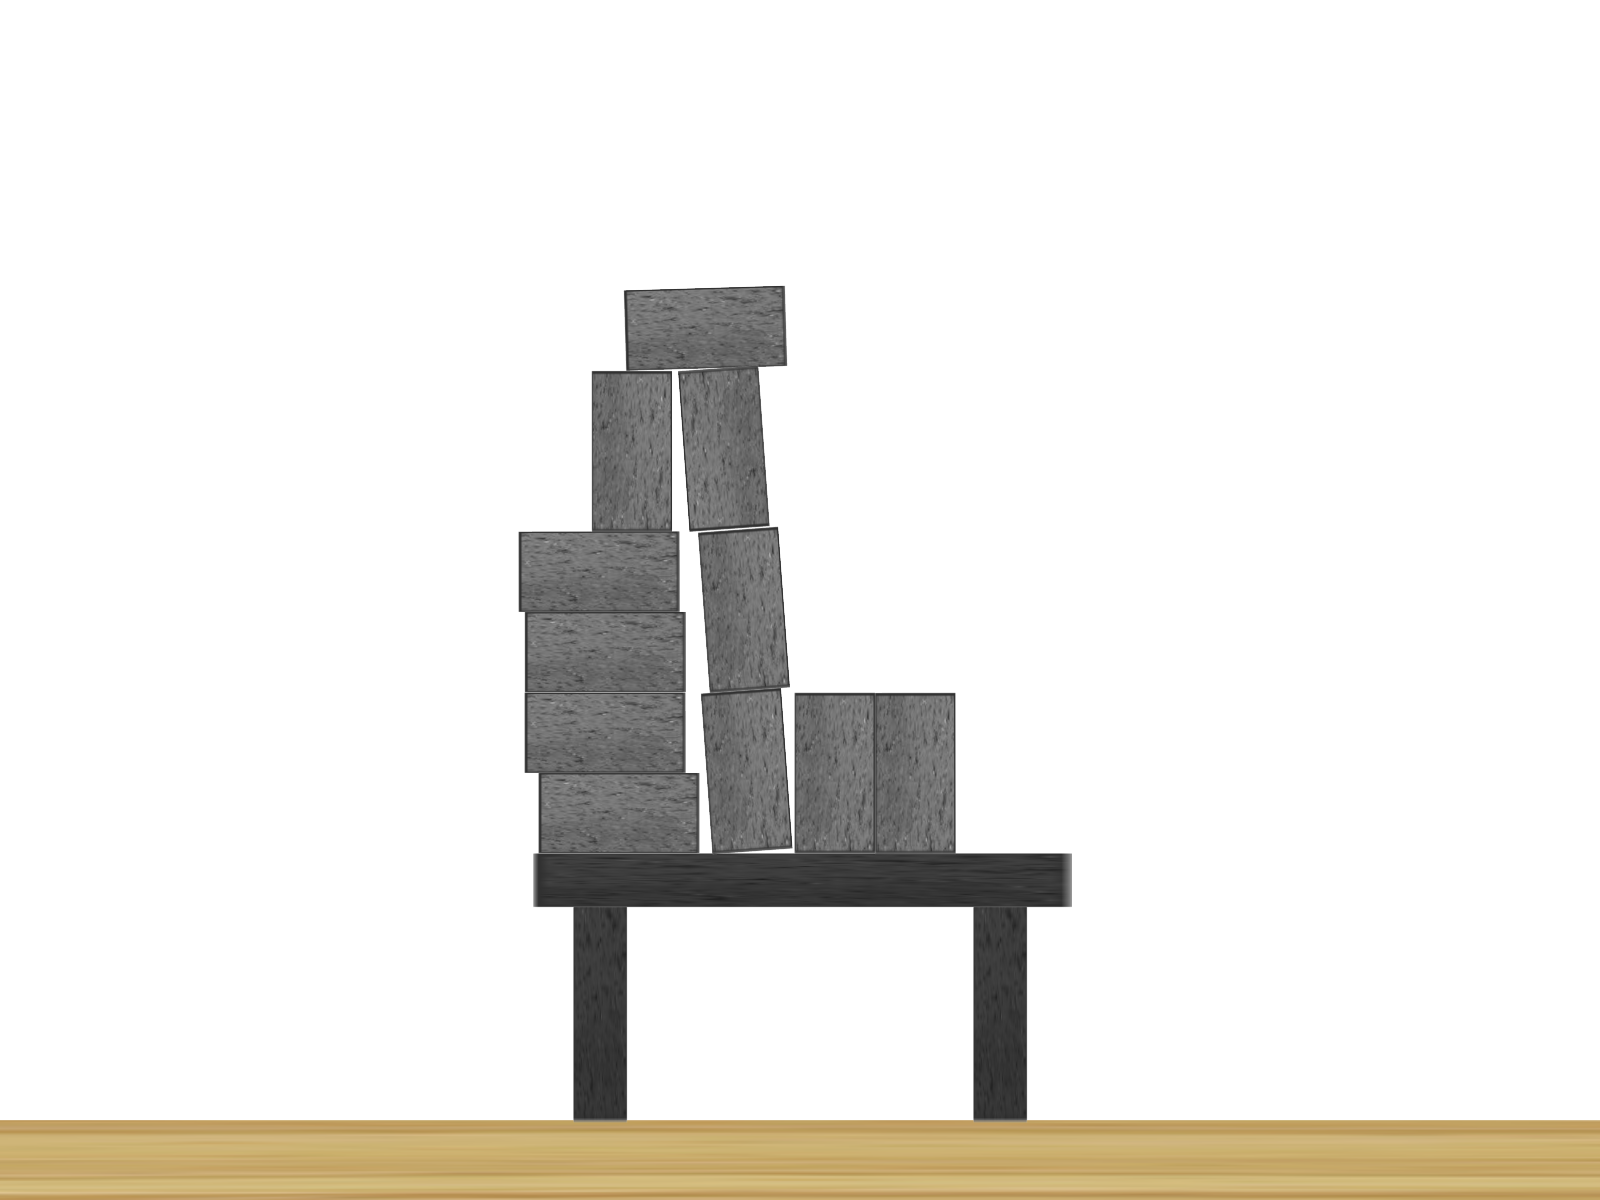
\includegraphics[width=0.2\columnwidth]{tower_image_after_(4)}}
% \hfill
% \subfloat[][fell \textbf{0}, changed \textbf{2}]{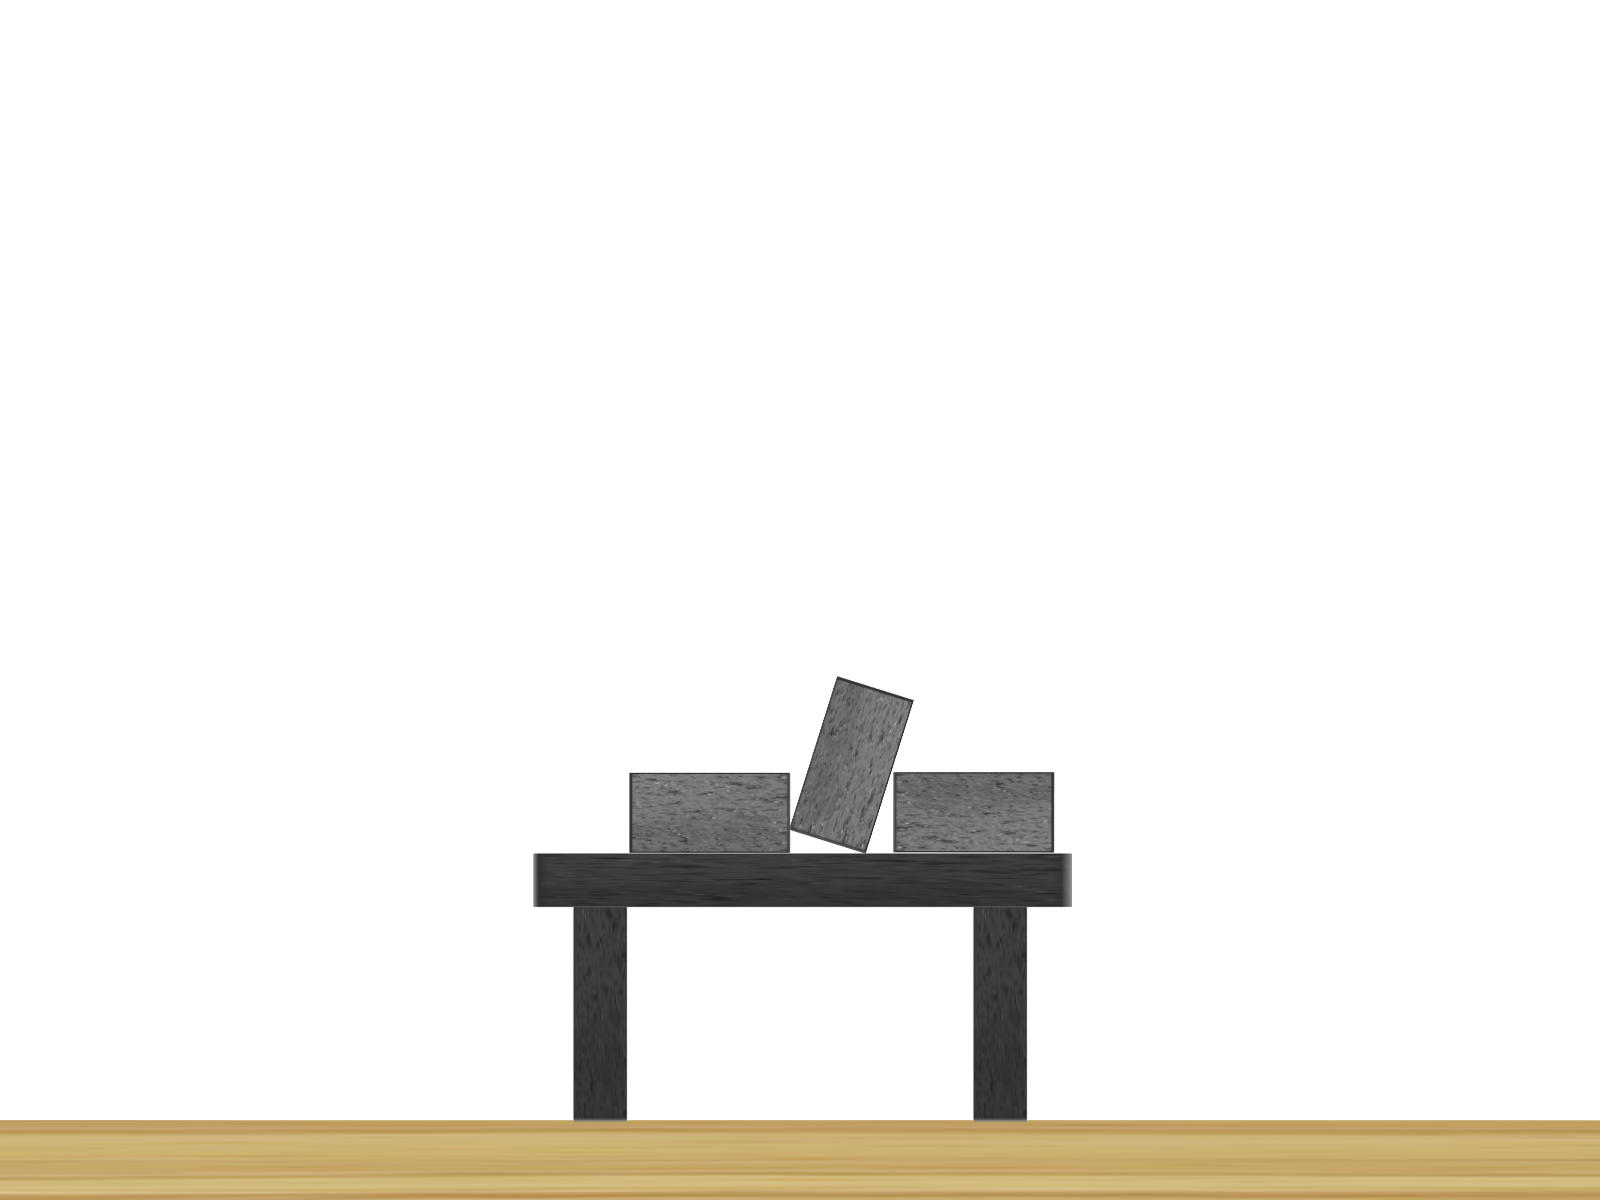
\includegraphics[width=0.2\columnwidth]{tower_image_after_(5)}}
% {\hfill}

% {\hfill}
% \subfloat[][fell \textbf{0}, changed \textbf{4}]{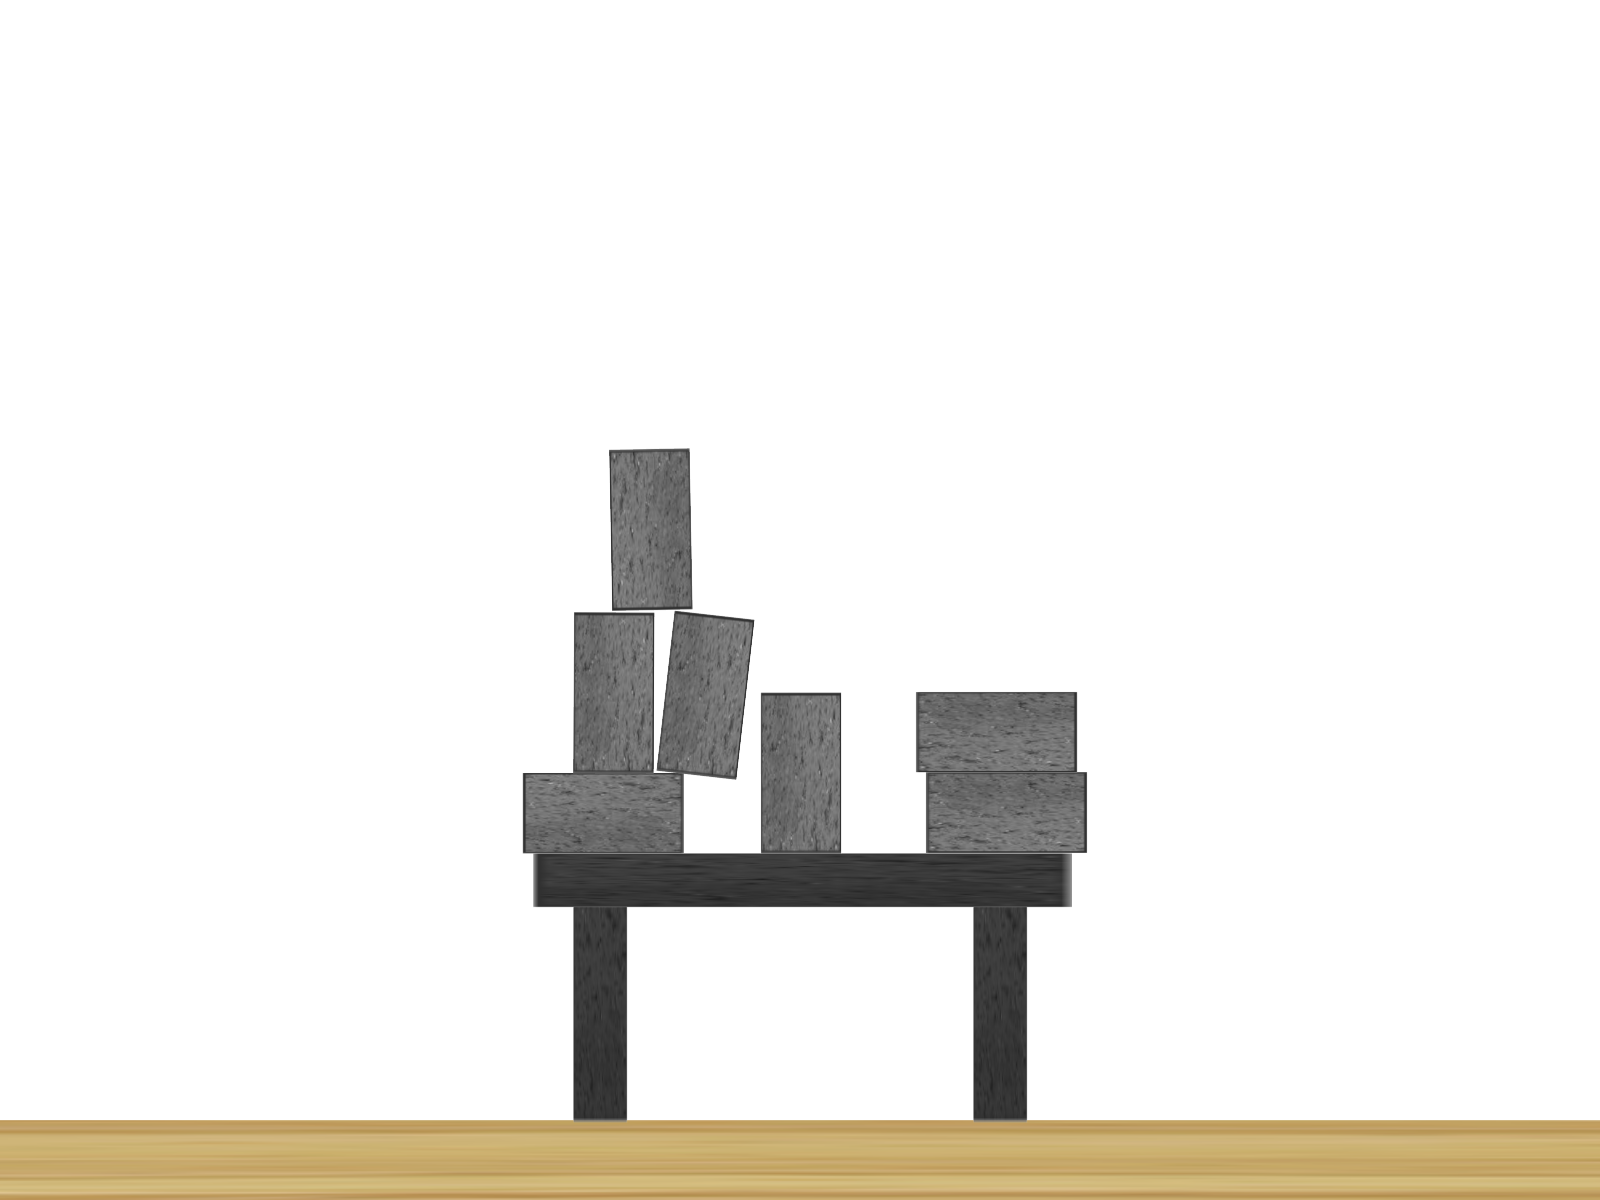
\includegraphics[width=0.2\columnwidth]{tower_image_after_(6)}}
% \hfill
% \subfloat[][fell \textbf{1}, changed \textbf{2}]{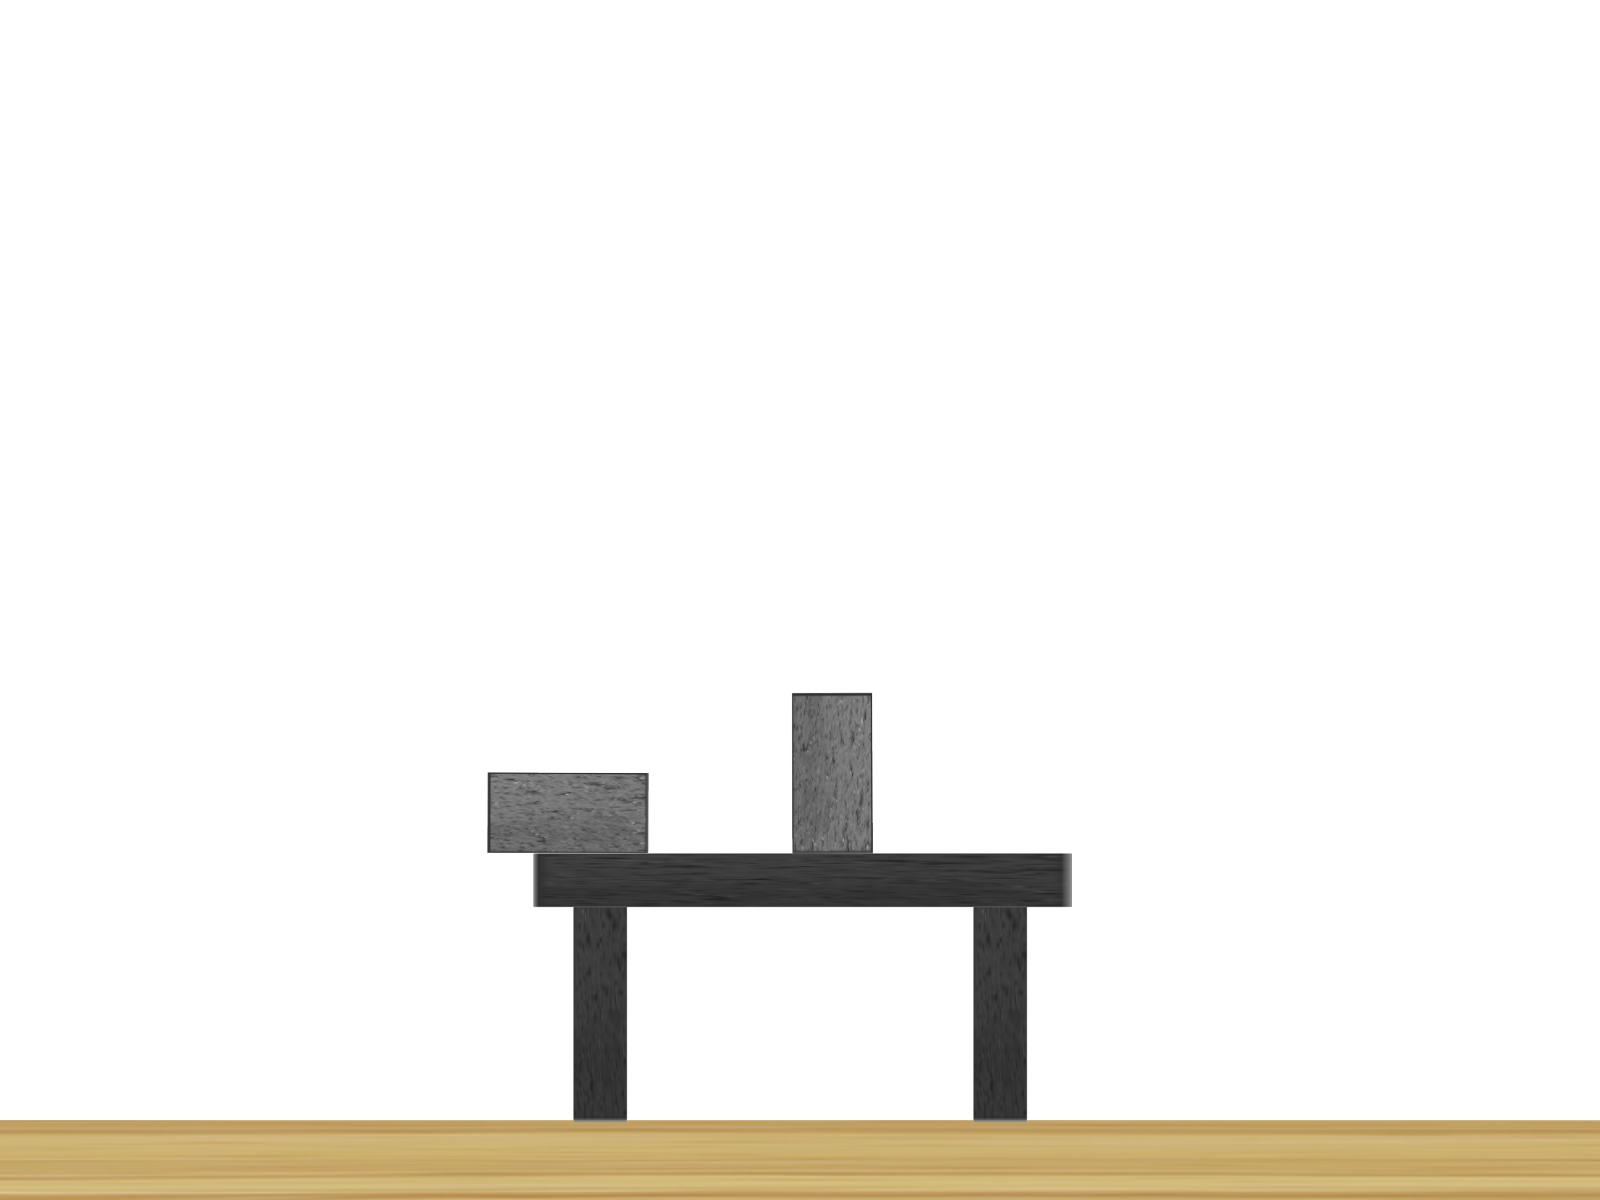
\includegraphics[width=0.2\columnwidth]{tower_image_after_(7)}}
% \hfill
% \subfloat[][fell \textbf{0}, changed \textbf{0}]{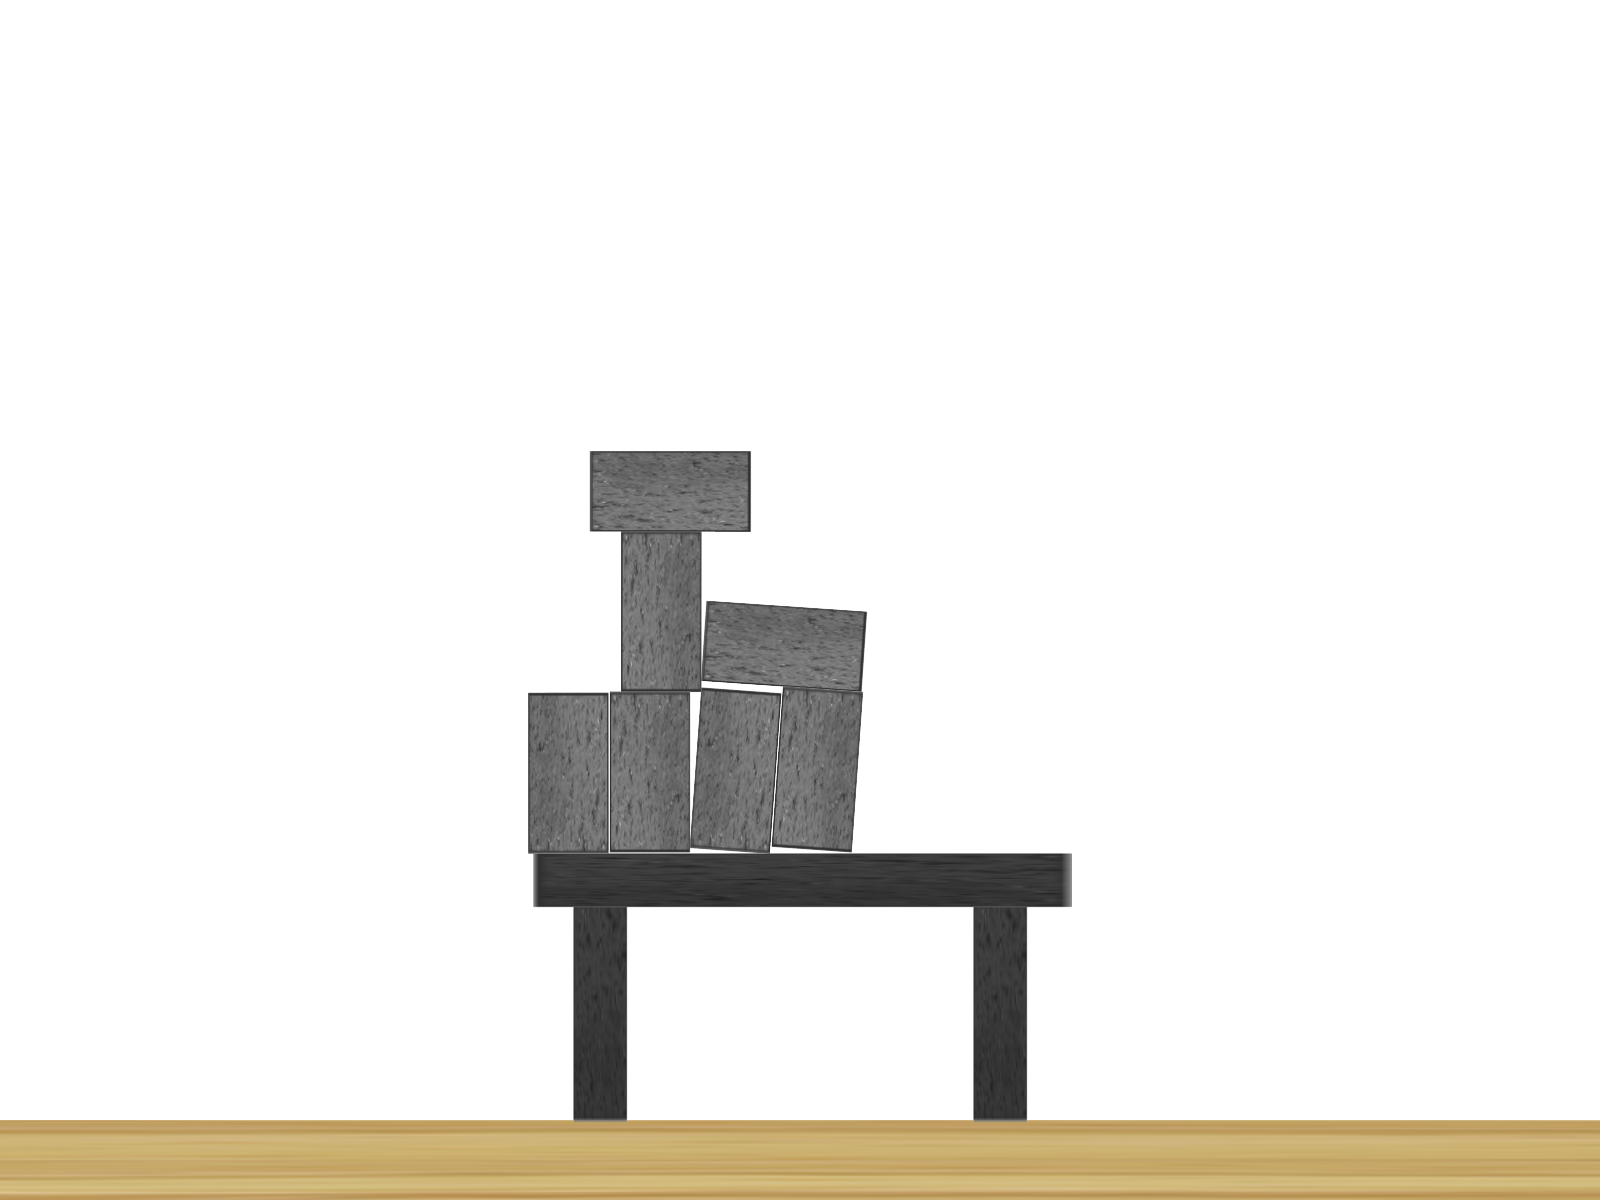
\includegraphics[width=0.2\columnwidth]{tower_image_after_(8)}}
% \hfill
% \subfloat[][fell \textbf{0}, changed \textbf{5}]{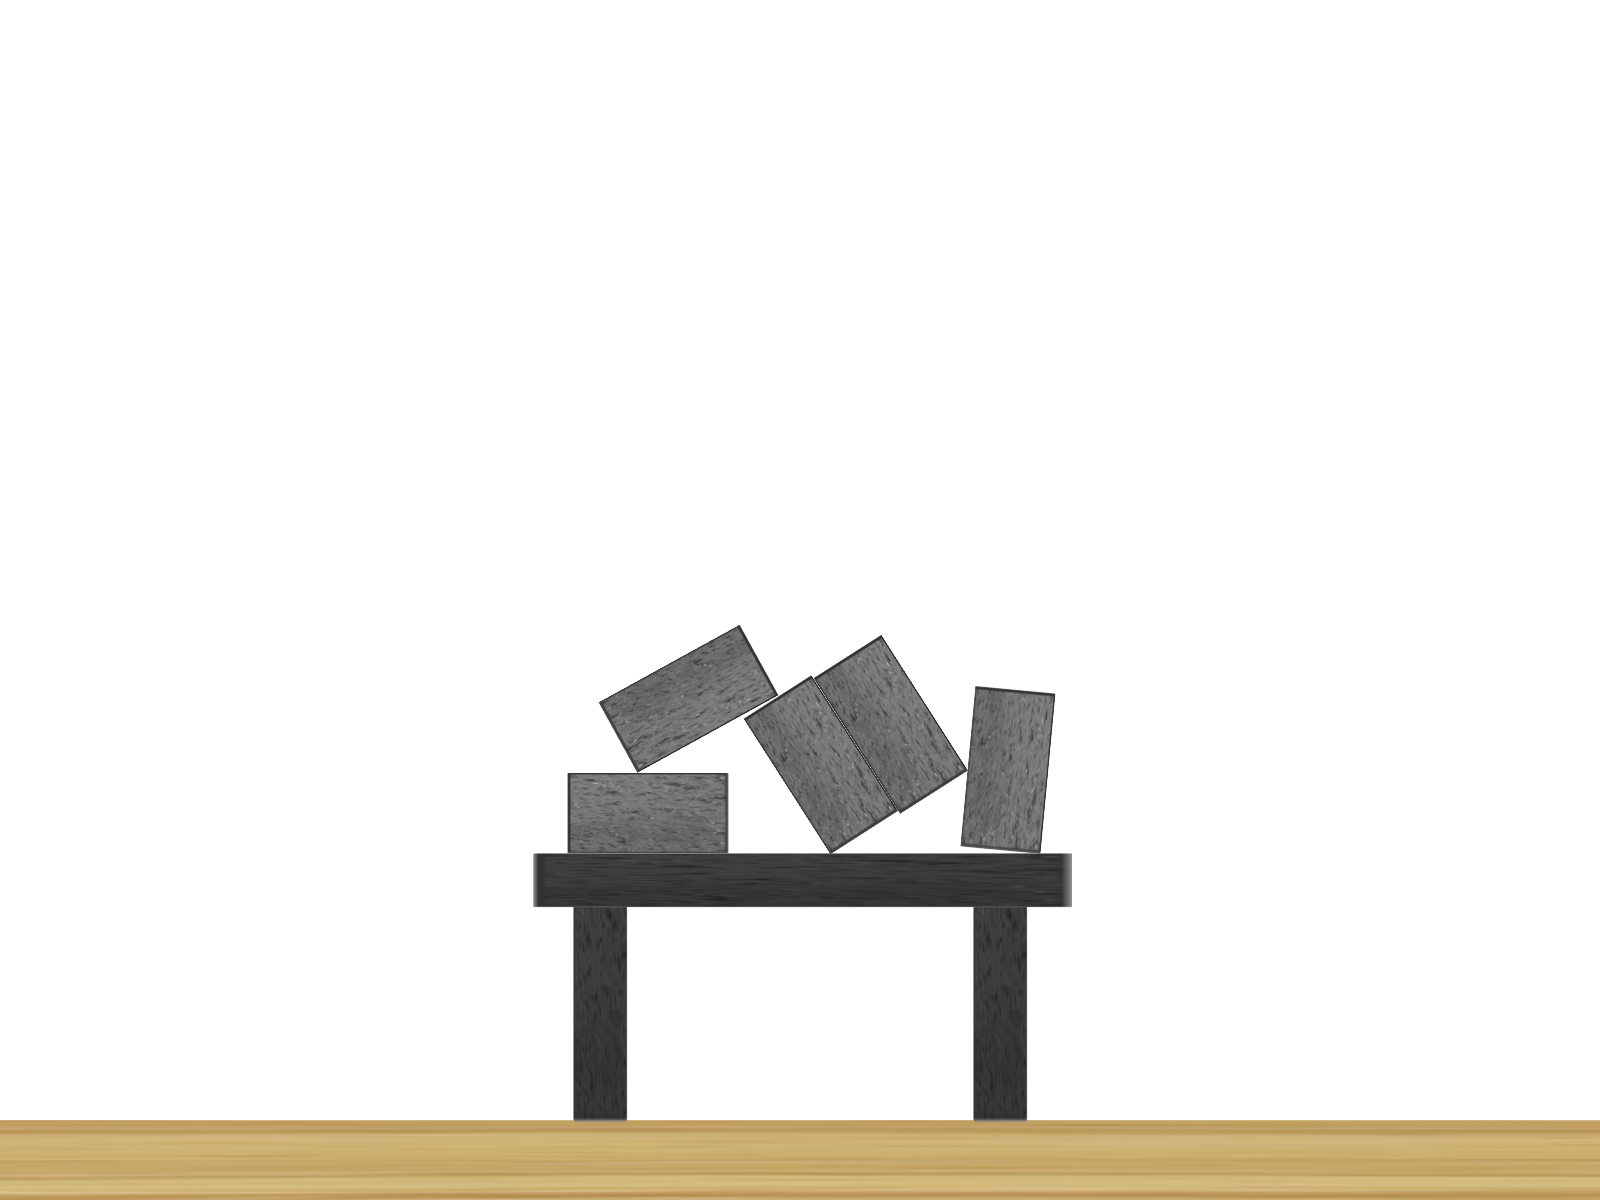
\includegraphics[width=0.2\columnwidth]{tower_image_after_(13)}}
% {\hfill}

% {\hfill}
% \subfloat[][fell \textbf{0}, changed \textbf{1}]{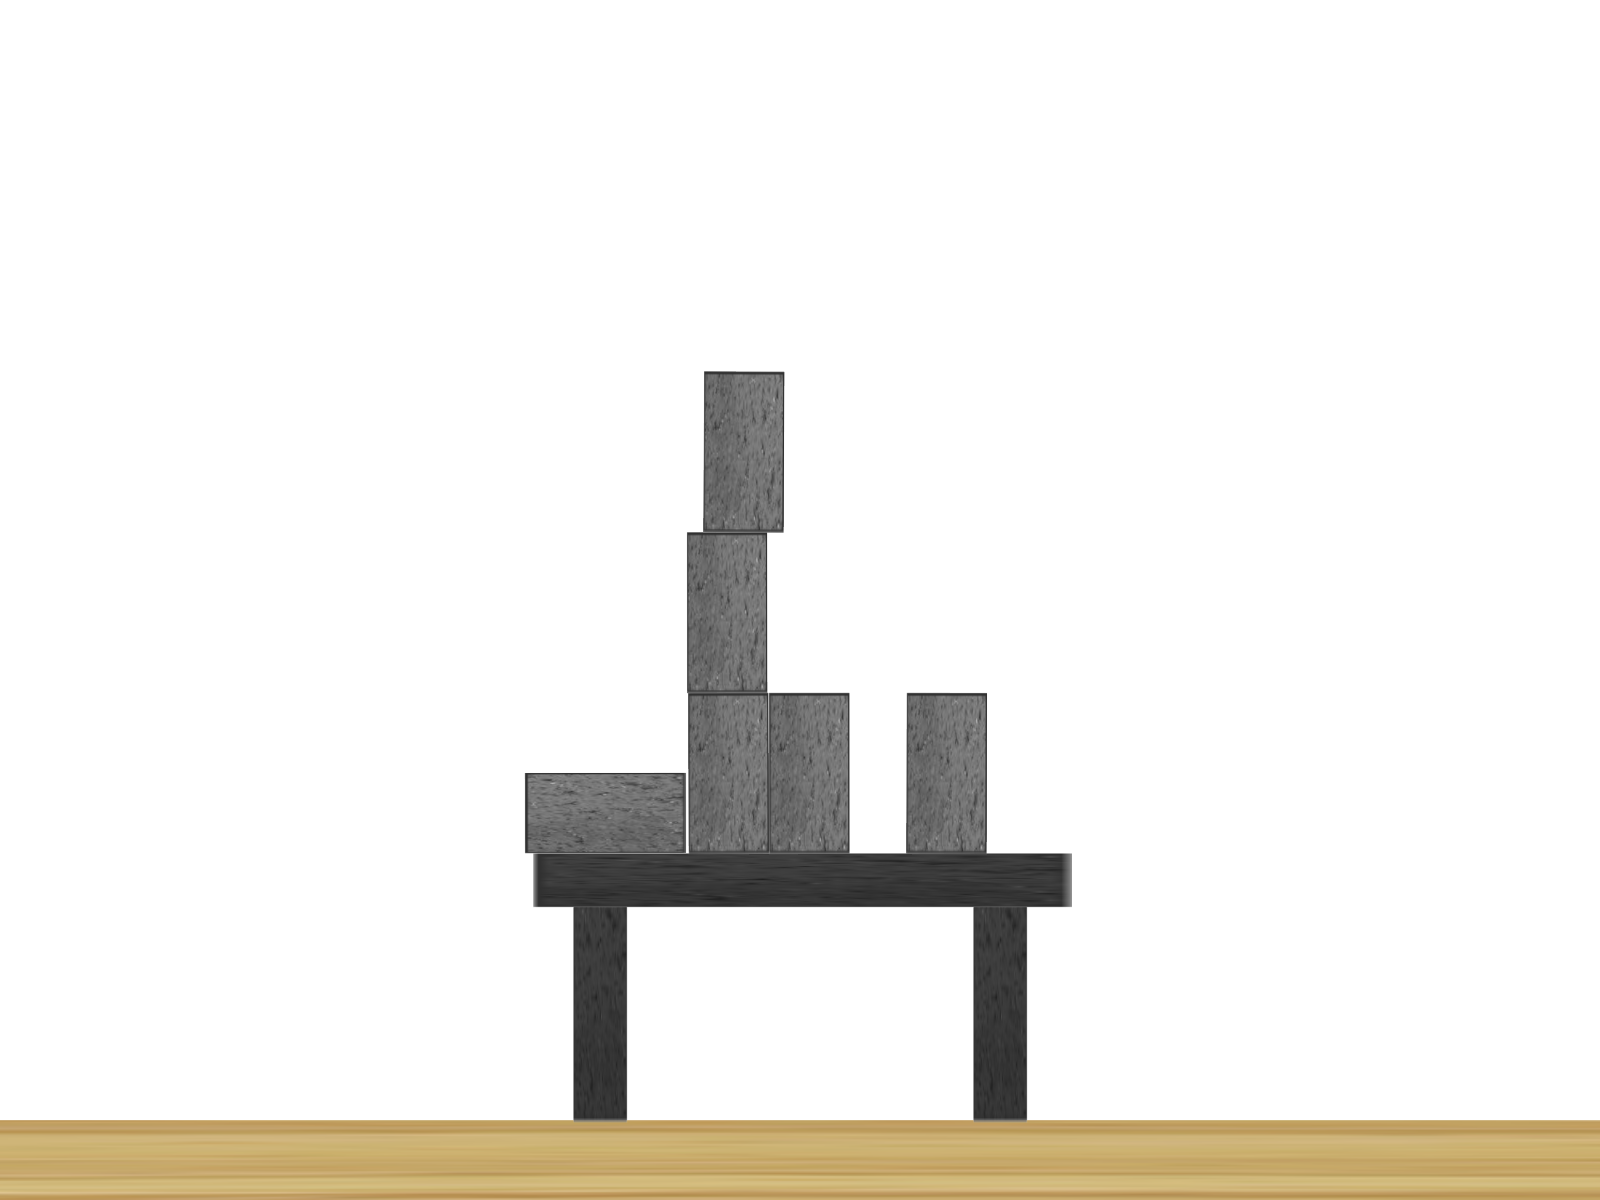
\includegraphics[width=0.2\columnwidth]{tower_image_after_(14)}}
% \hfill
% \subfloat[][fell \textbf{5}, changed \textbf{9}]{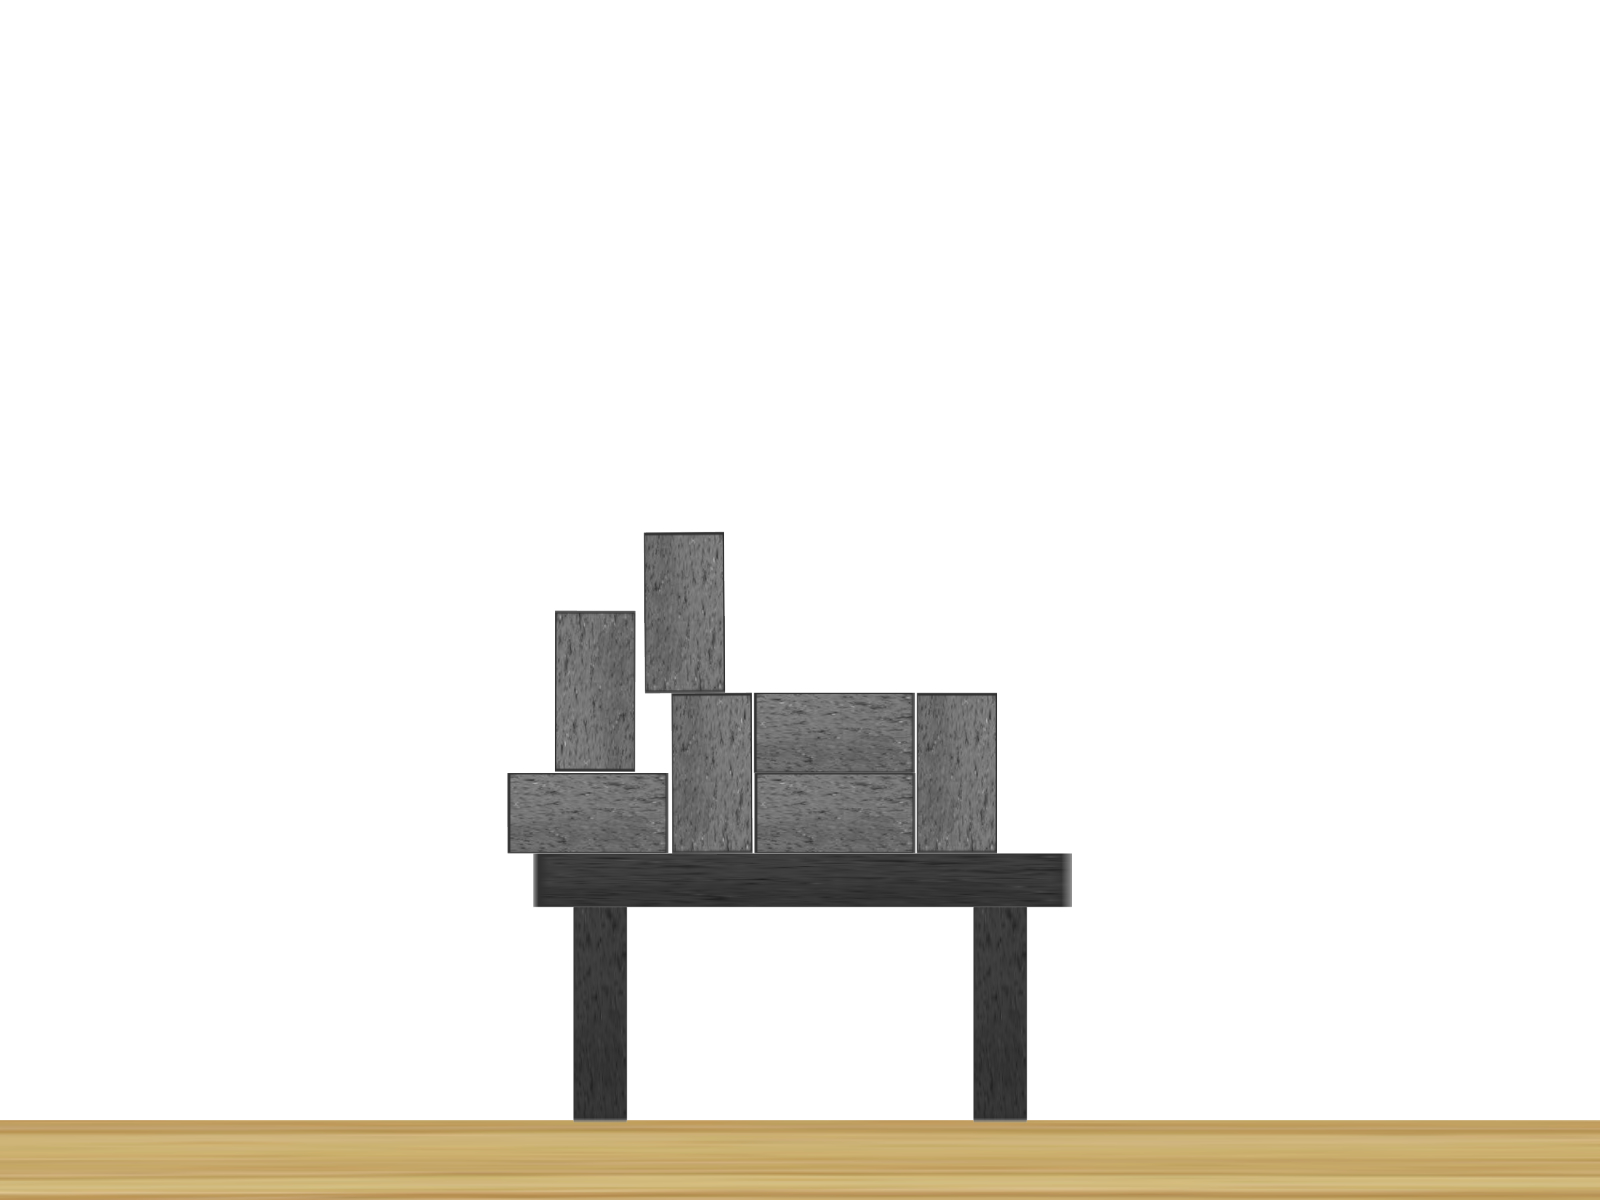
\includegraphics[width=0.2\columnwidth]{tower_image_after_(15)}}
% \hfill
% \subfloat[][fell \textbf{0}, changed \textbf{2}]{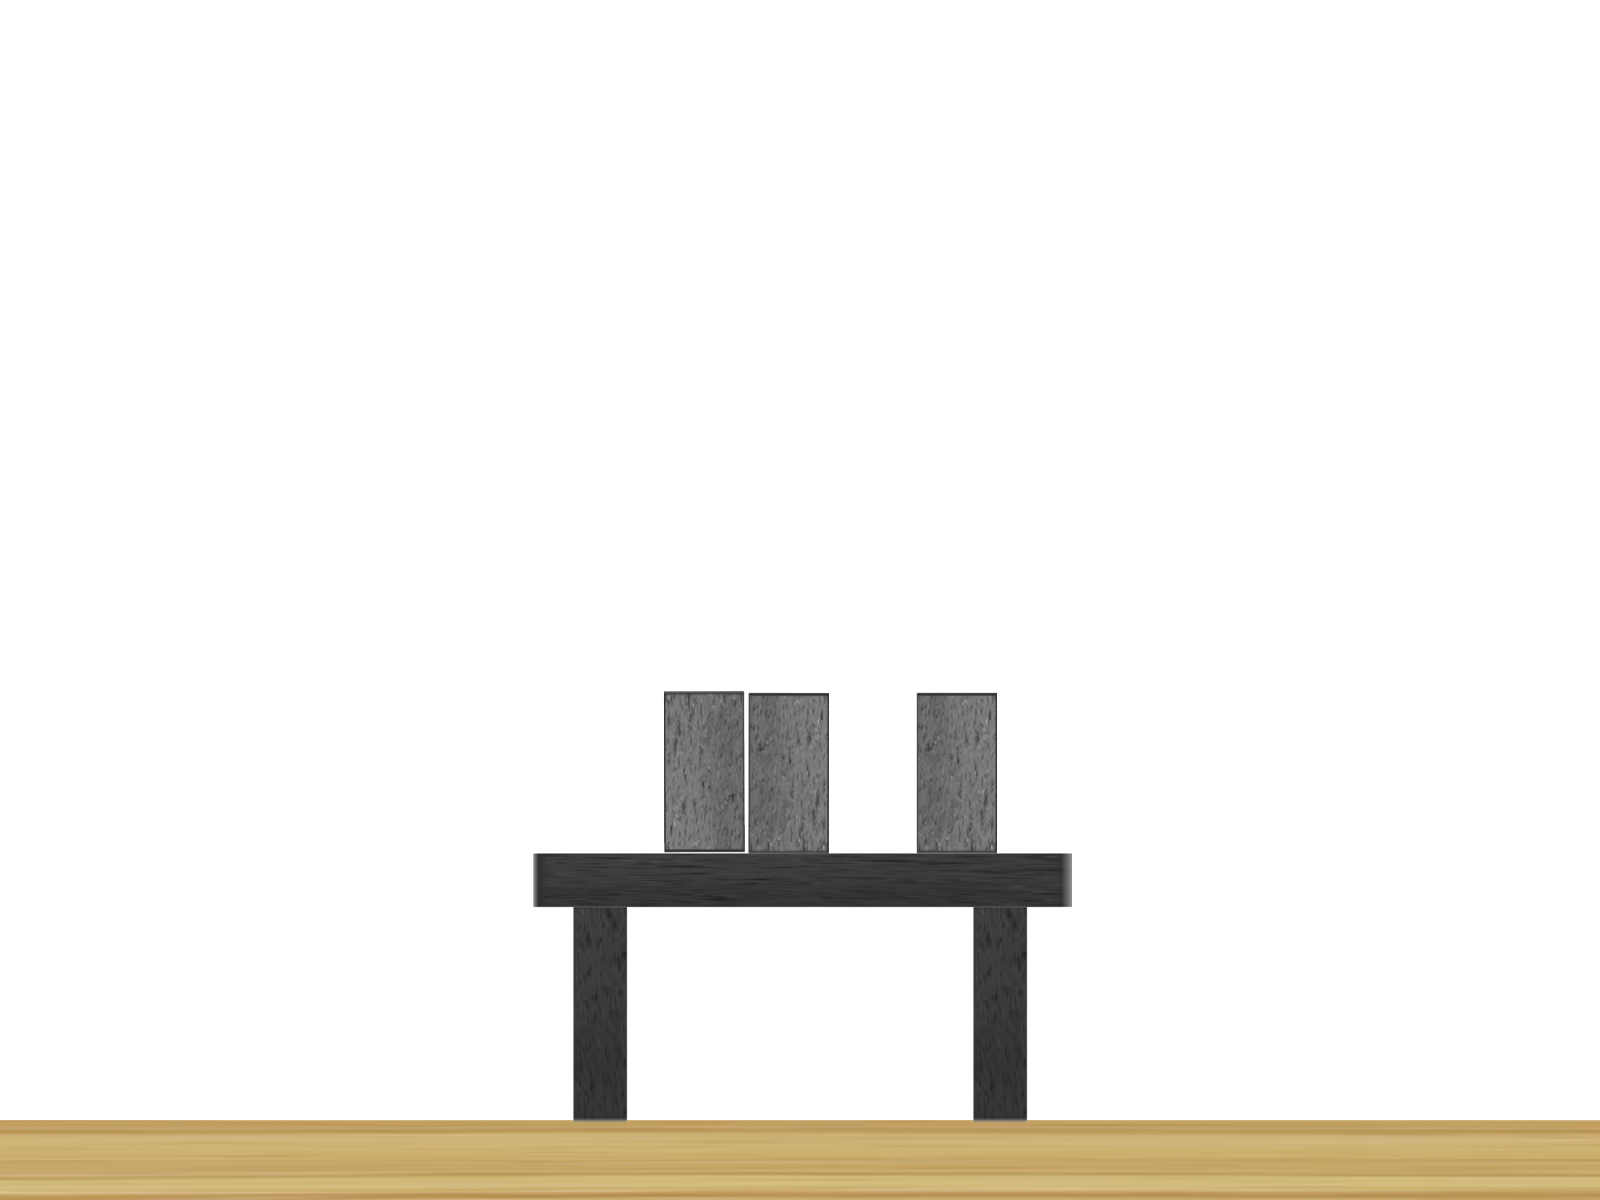
\includegraphics[width=0.2\columnwidth]{tower_image_after_(16)}}
% \hfill
% \subfloat[][fell \textbf{0}, changed \textbf{0}]{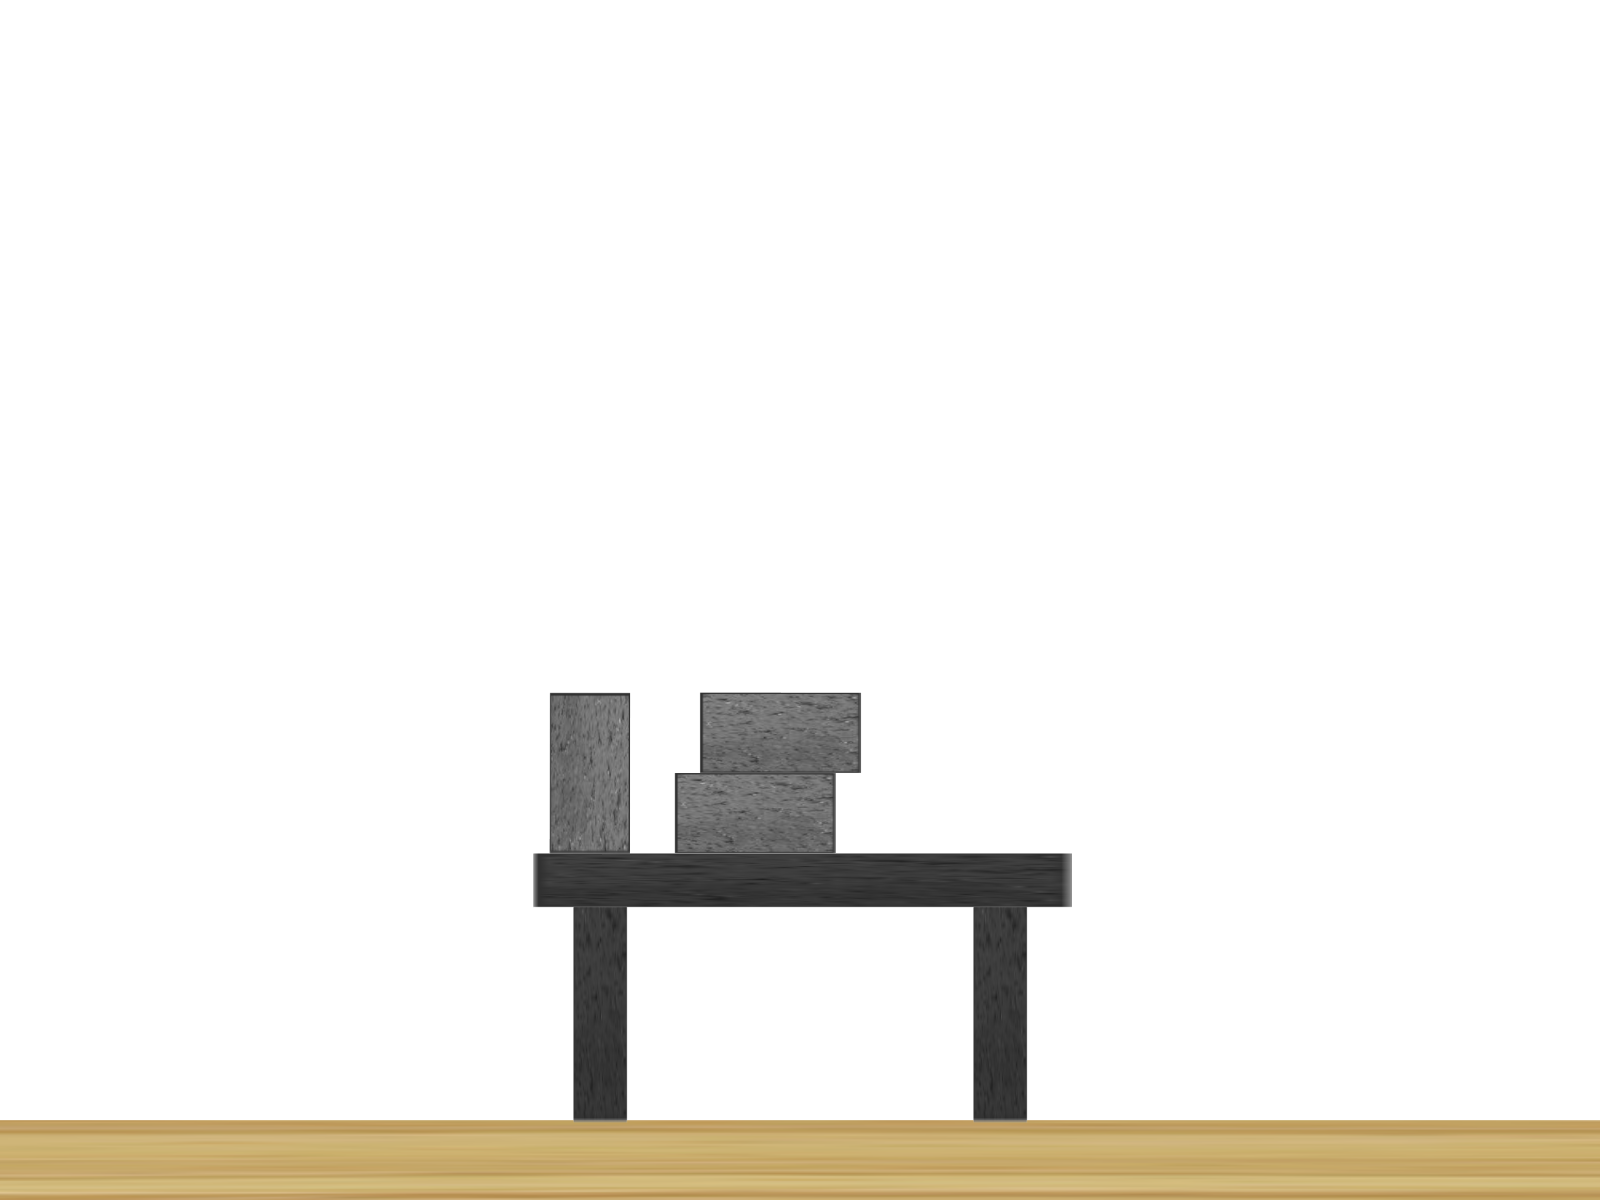
\includegraphics[width=0.2\columnwidth]{tower_image_after_(17)}}
% {\hfill}

% {\hfill}
% \subfloat[][fell \textbf{0}, changed \textbf{4}]{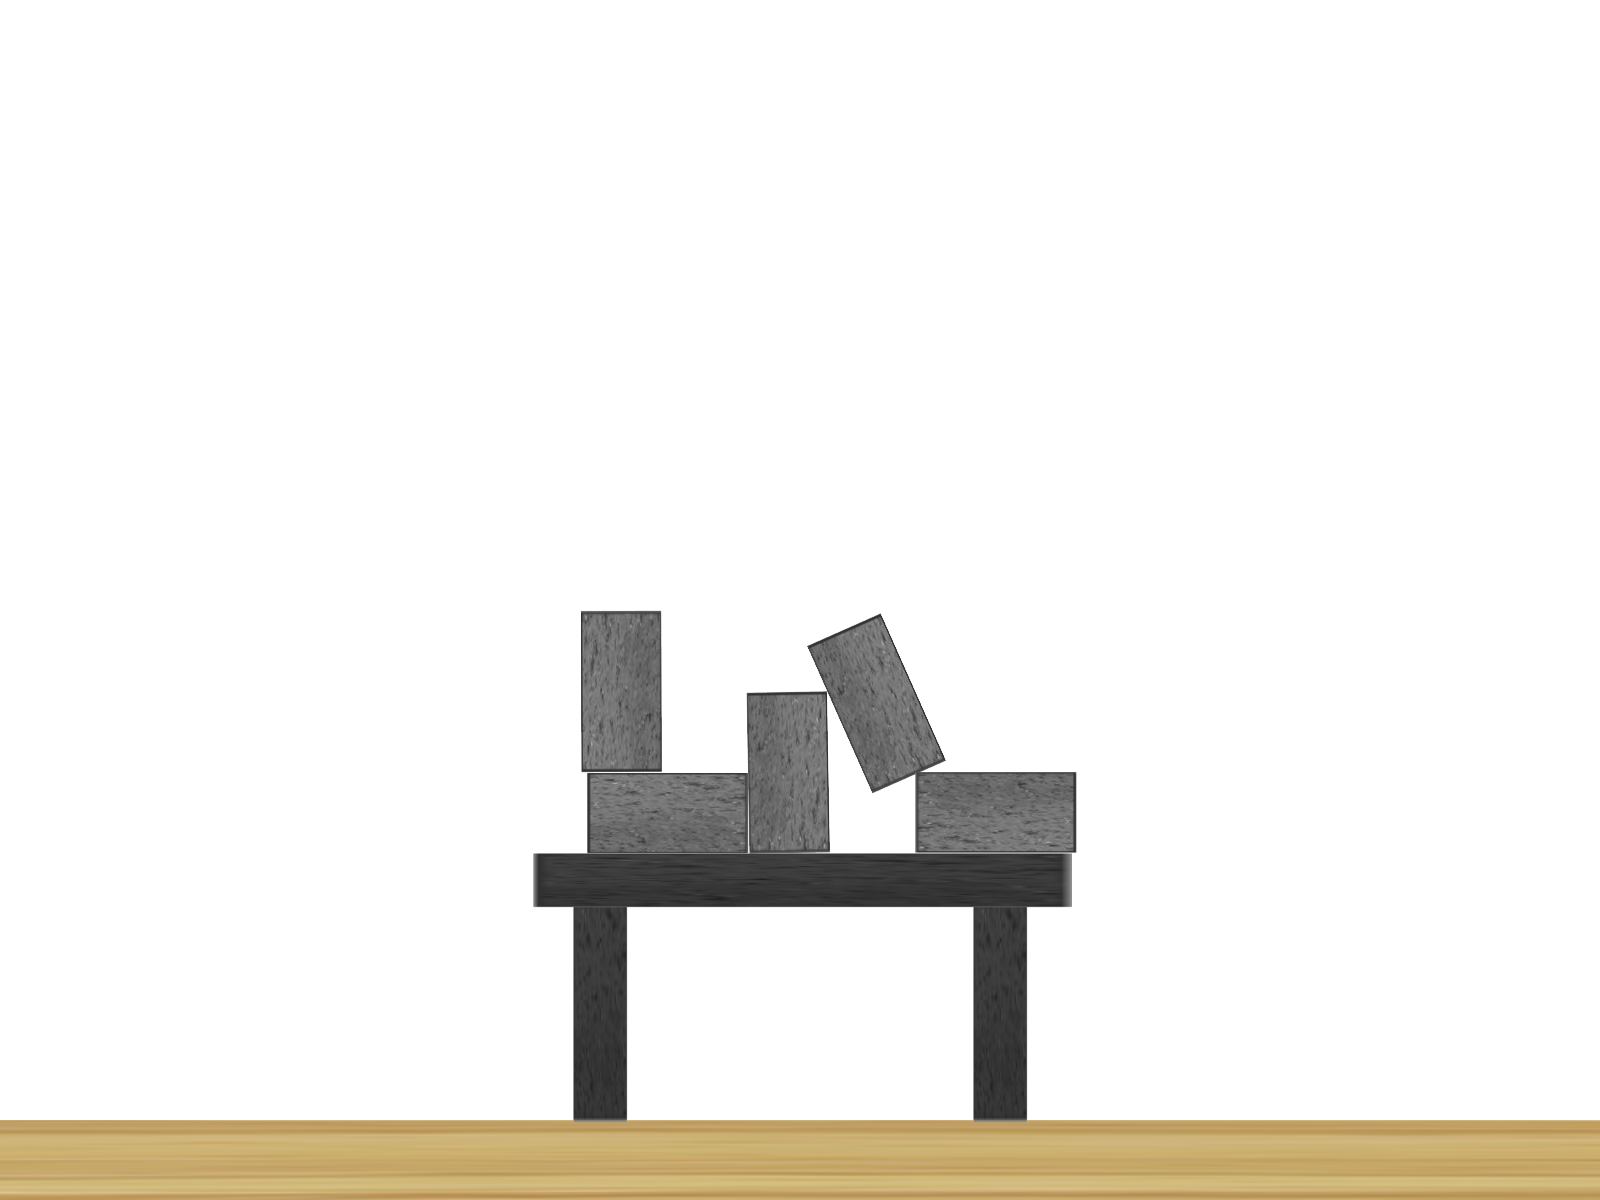
\includegraphics[width=0.2\columnwidth]{tower_image_after_(18)}}
% \hfill
% \subfloat[][fell \textbf{1}, changed \textbf{7}]{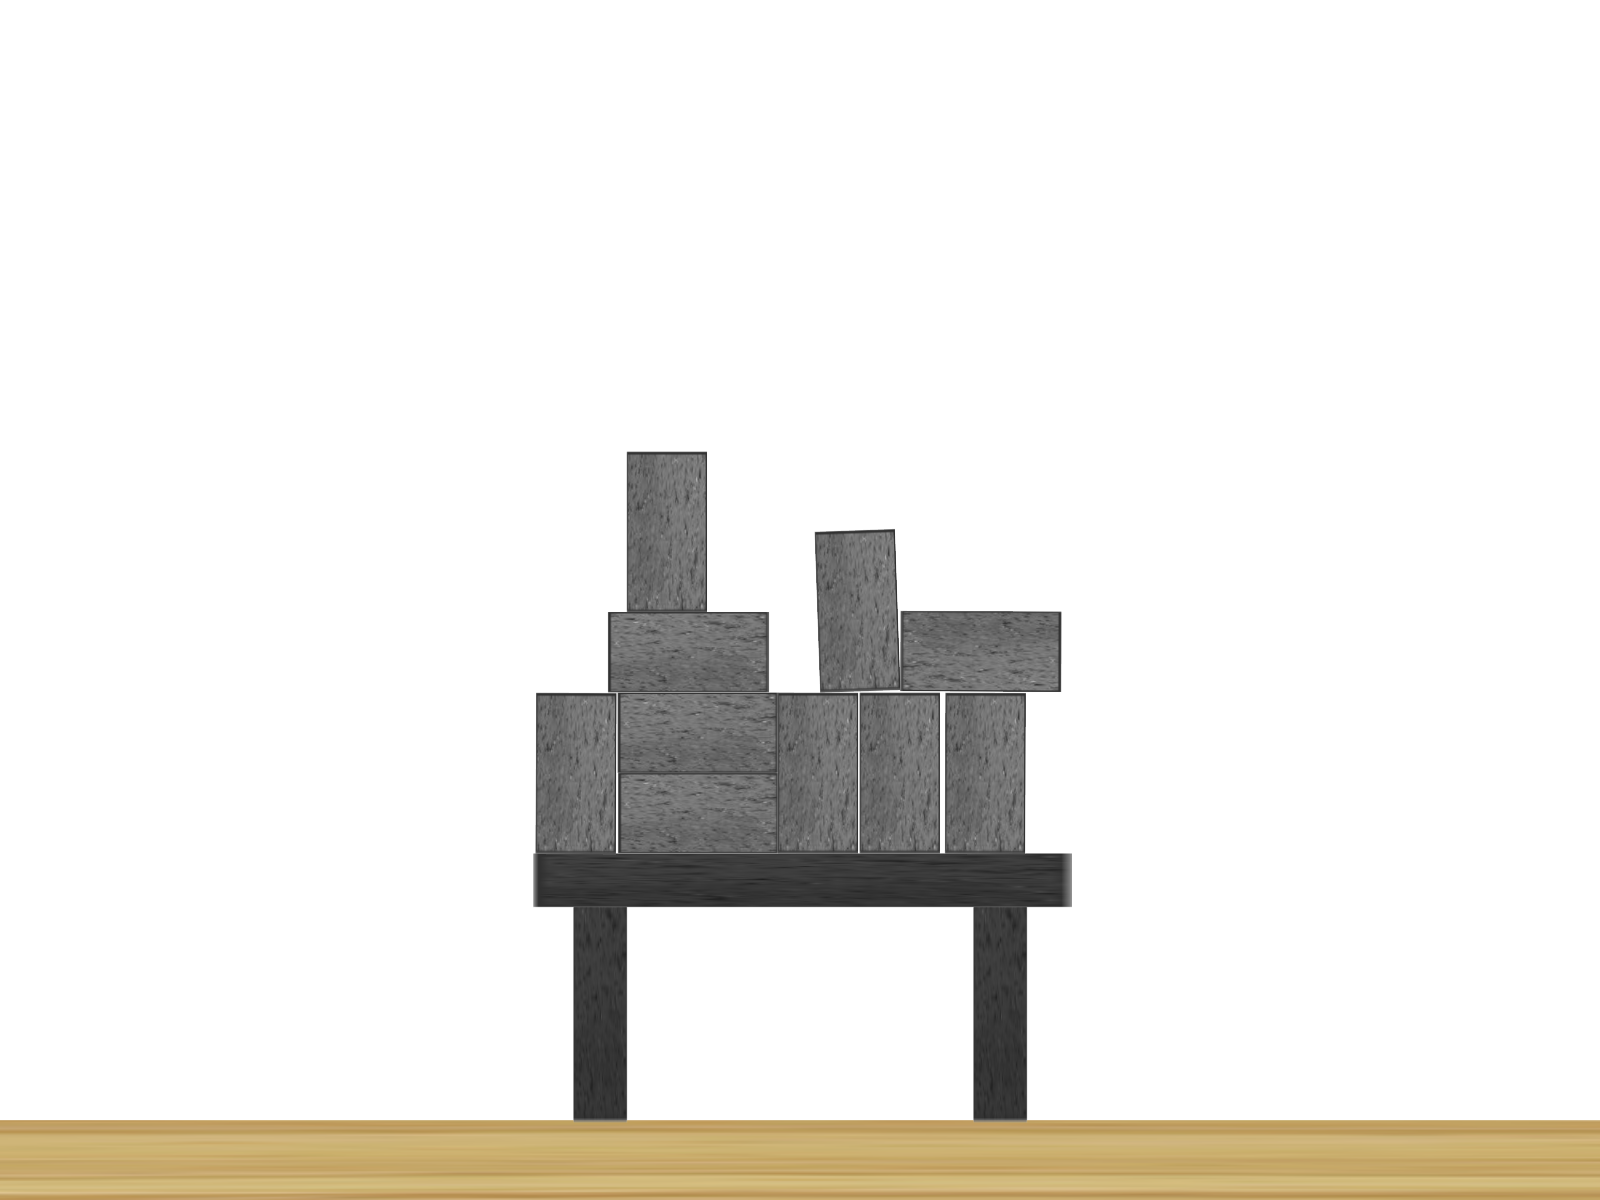
\includegraphics[width=0.2\columnwidth]{tower_image_after_(19)}}
% \hfill
% \subfloat[][fell \textbf{1}, changed \textbf{7}]{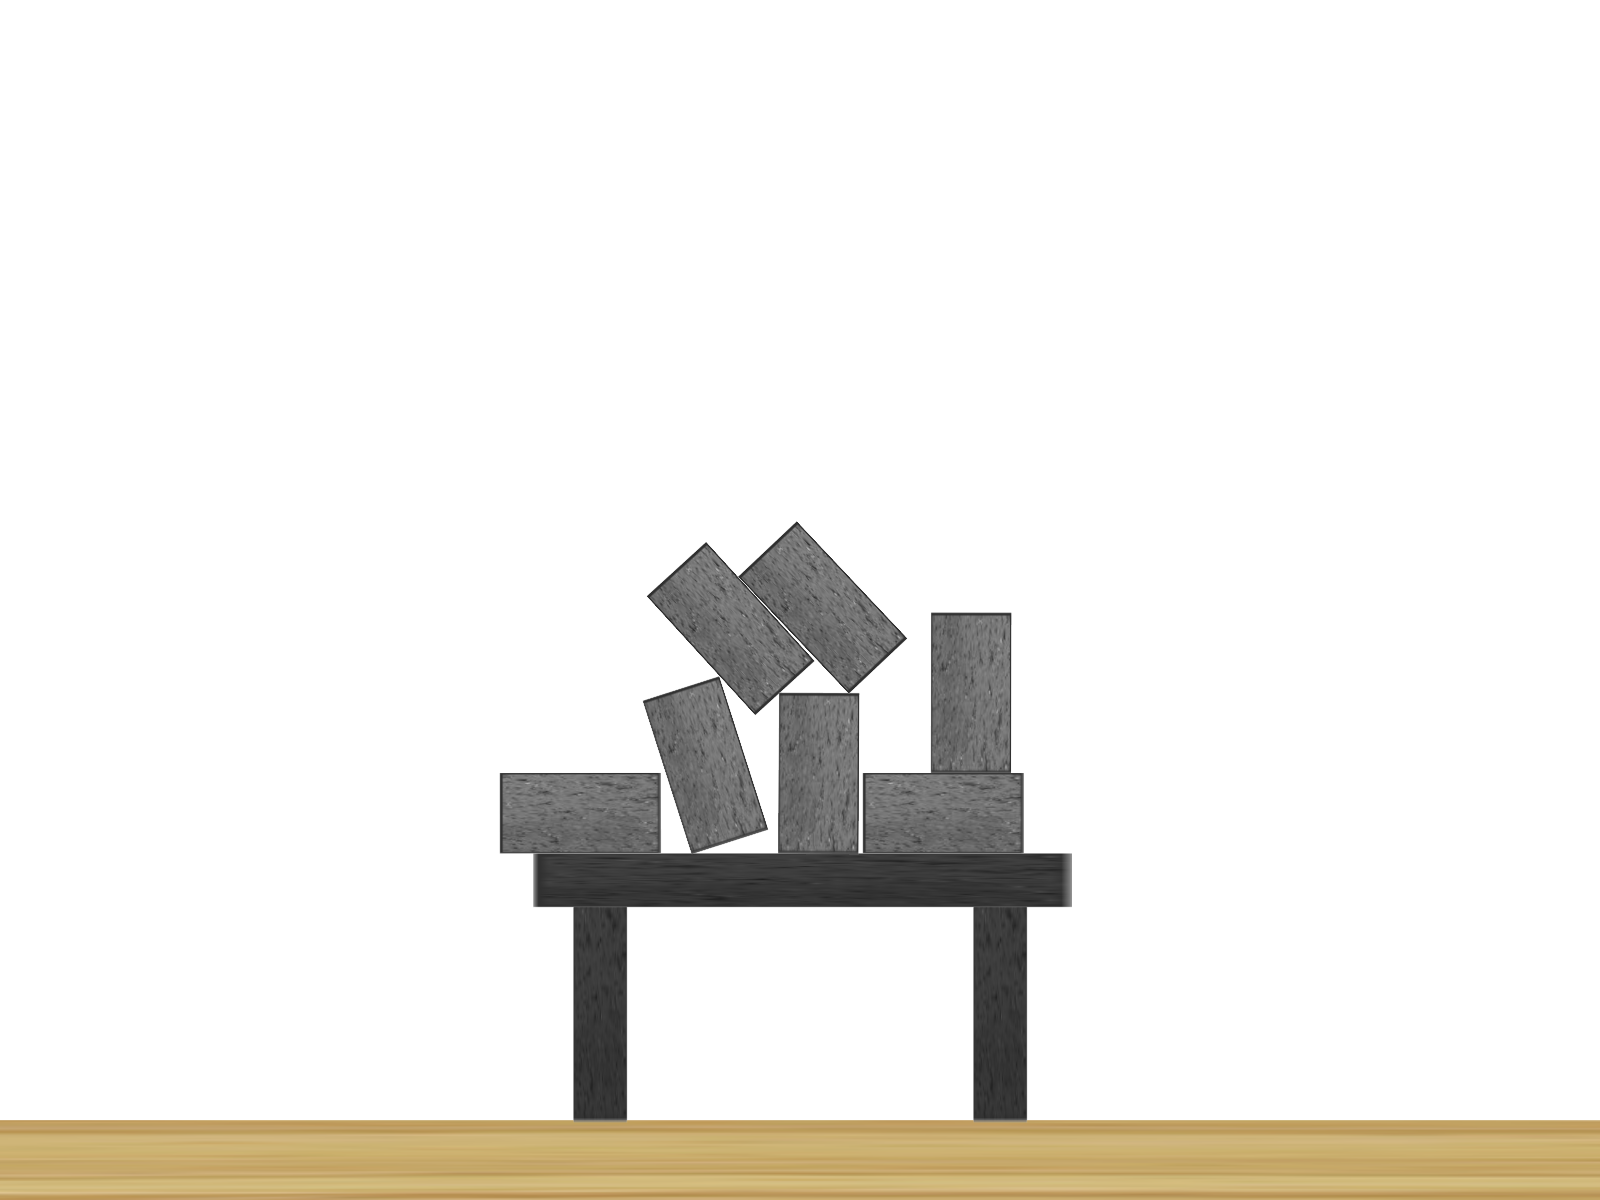
\includegraphics[width=0.2\columnwidth]{tower_image_after_(21)}}
% \hfill
% \subfloat[][fell \textbf{1}, changed \textbf{7}]{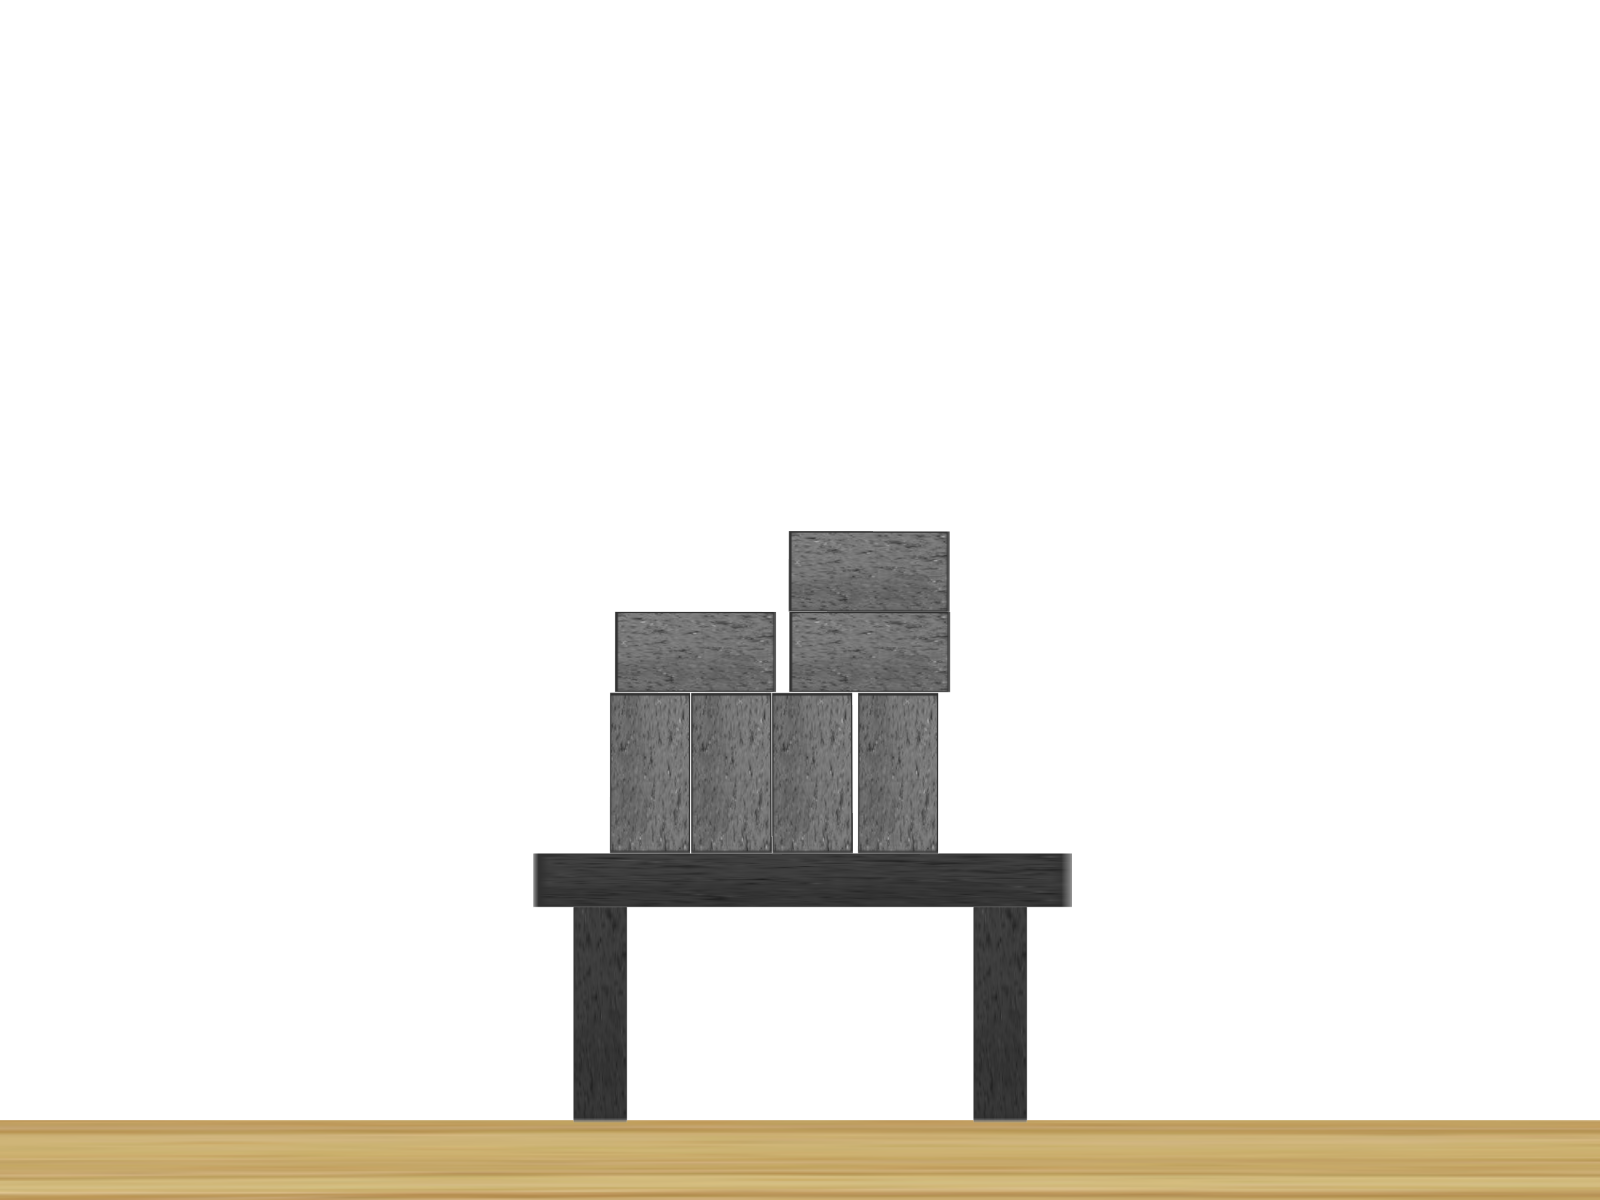
\includegraphics[width=0.2\columnwidth]{tower_image_after_(22)}}
% {\hfill}

% {\hfill}
% \subfloat[][fell \textbf{0}, changed \textbf{2}]{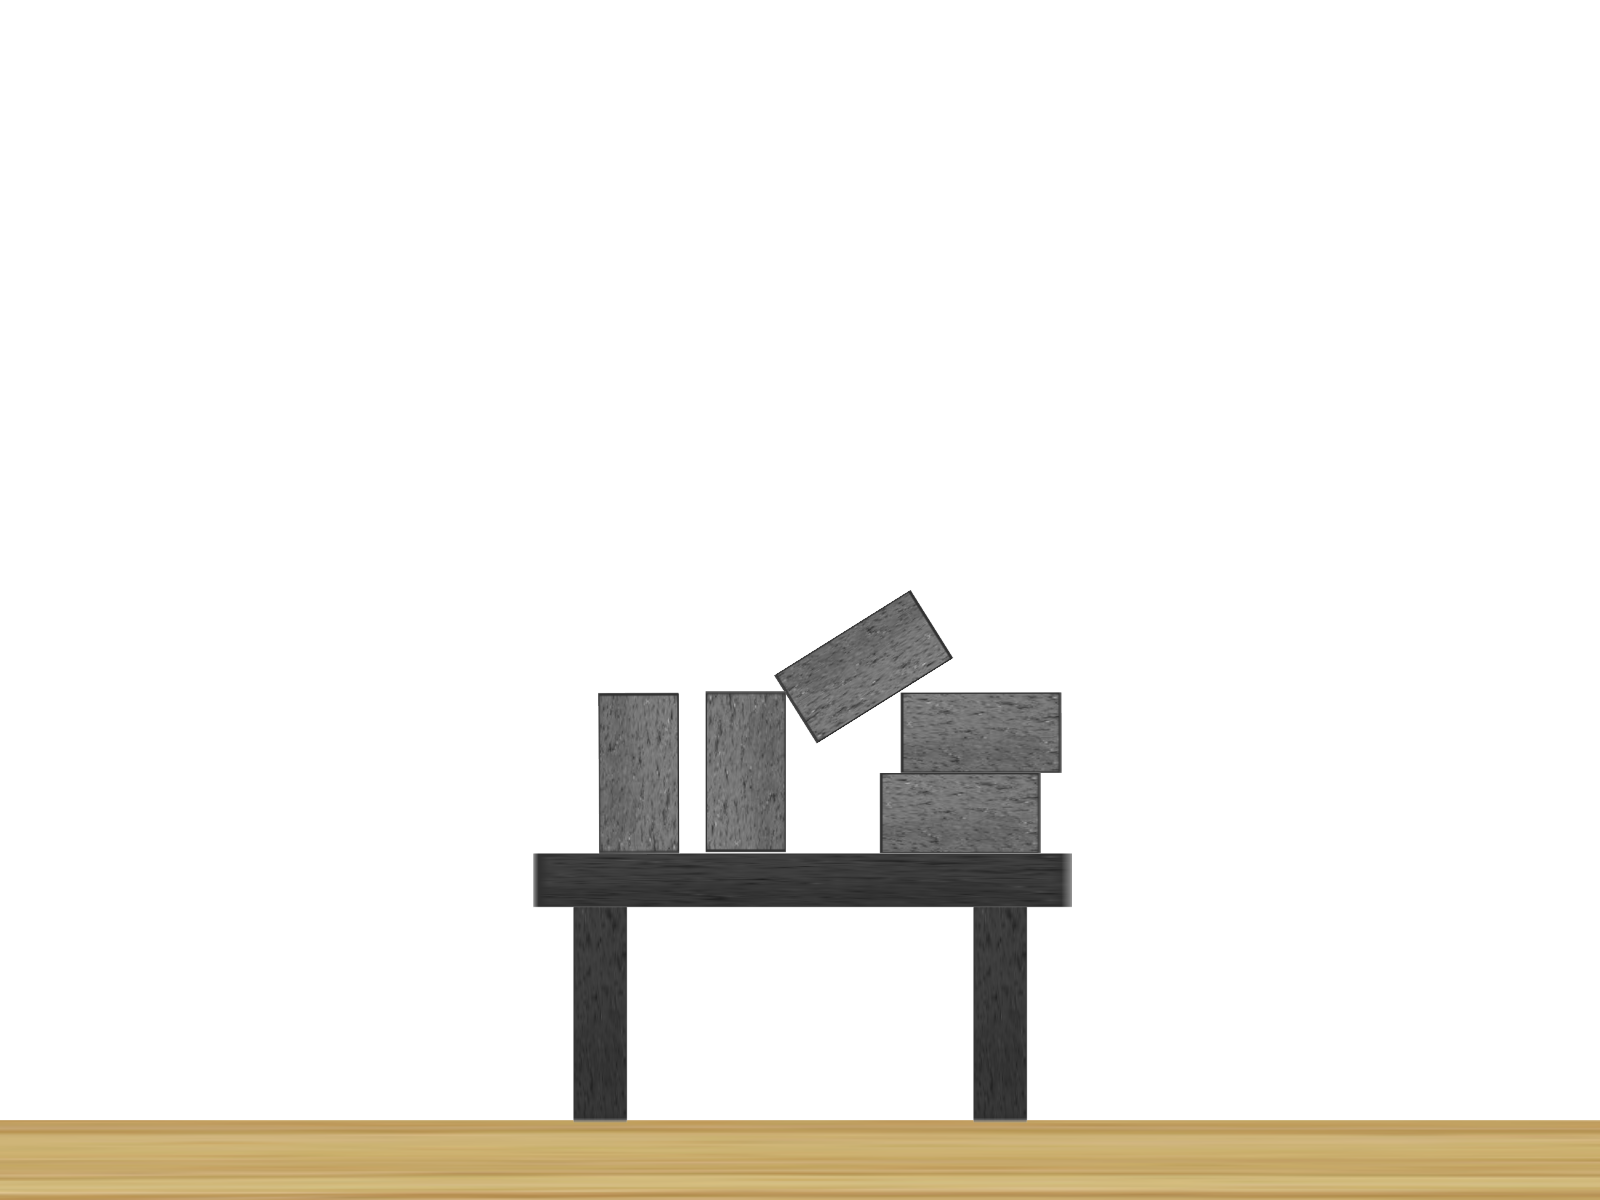
\includegraphics[width=0.2\columnwidth]{tower_image_after_(23)}}
% \hfill
% \subfloat[][fell \textbf{0}, changed \textbf{4}]{\includegraphics[width=0.2\columnwidth]{tower_image_after_(25)}}
% \hfill
% \subfloat[][fell \textbf{2}, changed \textbf{11}]{\includegraphics[width=0.2\columnwidth]{tower_image_after_(26)}}
% \hfill
% \subfloat[][fell \textbf{4}, changed \textbf{6}]{\includegraphics[width=0.2\columnwidth]{tower_image_after_(27)}}
% {\hfill}
% \end{figure}

% \begin{figure}[H]
% \renewcommand{\thesubfigure}{\arabic{subfigure}}
%  % \addtocounter{subfigure}{20} 
% {\hfill}
% \subfloat[][fell \textbf{0}, changed \textbf{0}]{\includegraphics[width=0.2\columnwidth]{tower_image_after_(28)}}
% \hfill
% \subfloat[][fell \textbf{0}, changed \textbf{1}]{\includegraphics[width=0.2\columnwidth]{tower_image_after_(29)}}
% \hfill
% \subfloat[][fell \textbf{0}, changed \textbf{7}]{\includegraphics[width=0.2\columnwidth]{tower_image_after_(30)}}
% \hfill
% \subfloat[][fell \textbf{2}, changed \textbf{12}]{\includegraphics[width=0.2\columnwidth]{tower_image_after_(31)}}
% {\hfill}

% {\hfill}
% \subfloat[][fell \textbf{0}, changed \textbf{2}]{\includegraphics[width=0.2\columnwidth]{tower_image_after_(32)}}
% \hfill
% \subfloat[][fell \textbf{3}, changed \textbf{6}]{\includegraphics[width=0.2\columnwidth]{tower_image_after_(33)}}
% \hfill
% \subfloat[][fell \textbf{2}, changed \textbf{4}]{\includegraphics[width=0.2\columnwidth]{tower_image_after_(34)}}
% \hfill
% \subfloat[][fell \textbf{2}, changed \textbf{4}]{\includegraphics[width=0.2\columnwidth]{tower_image_after_(35)}}
% {\hfill}

% {\hfill}
% \subfloat[][fell \textbf{0}, changed \textbf{2}]{\includegraphics[width=0.2\columnwidth]{tower_image_after_(36)}}
% \hfill
% \subfloat[][fell \textbf{4}, changed \textbf{10}]{\includegraphics[width=0.2\columnwidth]{tower_image_after_(37)}}
% {\hfill}
% \caption{Stimuli (after the brick was removed). \emph{Note}: \textbf{fell} = number of bricks that fell off the table, \textbf{changed} = number of bricks that changed their position.}
% \label{fig:stimuli_after}
% \end{figure}

% \subsection{Results}
% \label{sub:results}

% \begin{figure}[H]
%    \centering
%    \includegraphics[width = \columnwidth]{towers_model_whether_scatter}
%    \caption{Responsibility judgments and ground truth model that considers how many bricks \textbf{fell off the table}. \emph{Note}: The numbers indicate the different stimuli as shown in Figures \ref{fig:Stimuli} and \ref{fig:stimuli_after}.}
%    \label{fig:model_whether}
% \end{figure}

% \begin{figure}[H]
%    \centering
%    \includegraphics[width = \columnwidth]{towers_model_how_scatter}
%    \caption{Responsibility judgments and ground truth model that considers how many bricks \textbf{changed their position after the red brick was removed}.}
%    \label{fig:model_how}
% \end{figure}

% \begin{itemize}
%   \item A model that considers how many bricks would have changed their position if the red brick had been removed explains participants' responsibility judgments better than a model that considers how many bricks would have fallen off the table. 
%   \item \textbf{To do}: Look at models that introduce noise when the brick is removed.
% \end{itemize}

% % \begin{itemize}
% %   \item the model predicts participants' responsibility judgments as a function of (i) the number of blocks that fell off the table and (ii) the number of blocks that changed their position 
% % \end{itemize}

% % \begin{itemize}
% %   \item both whether and how may be of relevance 
% %   \item lowest responsibility when block makes no difference whatsoever 
% %   \item responsibility when there is how-dependence but no whether-dependence
% % \end{itemize}

% % \begin{itemize}
% %   \item noise model 
% %   \begin{itemize}
% %     \item perceptual noise 
% %     \item friction noise 
% %   \end{itemize}
% %   \begin{itemize}
% %     \item number of blocks 
% %     \item proportion of blocks 
% %   \end{itemize}
% % \end{itemize}

% % \clearpage
% % \section{To do list}
% % \label{sec:to_do_list}

% % \begin{itemize}
% % 	\item write code that determines for each clip how many blocks would have fallen 
% % 	\begin{itemize}
% % 		\item think about how to introduce noise to capture uncertainty 
% % 	\end{itemize}
% % \end{itemize}

% \clearpage
% \section{Experiment 2: Prediction \& Responsibility}
% \label{sec:experiment_2}

% \subsection{Methods}
% \label{sub:methods}

% \subsubsection{Design}
% \label{ssub:design}

% \begin{itemize}
%   \item \emph{Prediction condition}: How many of the \textbf{\color[rgb]{.6,0,0}red bricks} would fall off the table, if the \textbf{black brick} wasn't there?
%   \item \emph{Responsibility condition}: How responsible is the \textbf{black brick} for the \textbf{\color[rgb]{.6,0,0}red bricks} staying on the table?
% \end{itemize}

% \subsubsection{Procedure}
% \label{ssub:procedure}


% \begin{figure}[H]
% \centering
% {\hfill}
% \subfloat[][Instructions]{\includegraphics[width=0.32\columnwidth]{exp2_screenshot_1}}
% \hfill
% \subfloat[][Observations]{\includegraphics[width=0.32\columnwidth]{exp2_screenshot_2}}
% \hfill
% \subfloat[][Responsibility judgments / Counterfactual prediction.]{\includegraphics[width=0.32\columnwidth]{exp2_screenshot_3}}
% {\hfill}
% \caption{Experiment screenshots.}
% \label{fig:label}
% \end{figure}


% \clearpage
% \subsubsection{Stimuli}
% \label{ssub:stimuli}

% \centerline{Difference: 0}
% \vspace{-0.5cm}
% \begin{figure}[H]
% \renewcommand{\thesubfigure}{\arabic{subfigure}}
% \centering
% {\hfill}
% \subfloat[][]{\includegraphics[width=0.16\columnwidth]{initial_trial_1}}
% \hfill
% \subfloat[][]{\includegraphics[width=0.16\columnwidth]{initial_trial_2}}
% \hfill
% \subfloat[][]{\includegraphics[width=0.16\columnwidth]{initial_trial_3}}
% \hfill
% \subfloat[][]{\includegraphics[width=0.16\columnwidth]{initial_trial_4}}
% \hfill
% \subfloat[][]{\includegraphics[width=0.16\columnwidth]{initial_trial_5}}
% \hfill
% \subfloat[][]{\includegraphics[width=0.16\columnwidth]{initial_trial_6}}
% {\hfill}
% \end{figure}
% \vspace{-0.5cm}
% \centerline{Difference: 1}
% \vspace{-0.5cm}
% \begin{figure}[H]
% \renewcommand{\thesubfigure}{\arabic{subfigure}}
% %\captionsetup[subfigure]{labelformat=empty}
% \centering
% {\hfill}
% \subfloat[][]{\includegraphics[width=0.16\columnwidth]{initial_trial_7}}
% \hfill
% \subfloat[][]{\includegraphics[width=0.16\columnwidth]{initial_trial_8}}
% \hfill
% \subfloat[][]{\includegraphics[width=0.16\columnwidth]{initial_trial_9}}
% \hfill
% \subfloat[][]{\includegraphics[width=0.16\columnwidth]{initial_trial_10}}
% \hfill
% \subfloat[][]{\includegraphics[width=0.16\columnwidth]{initial_trial_11}}
% \hfill
% \subfloat[][]{\includegraphics[width=0.16\columnwidth]{initial_trial_12}}
% {\hfill}
% \end{figure}
% \vspace{-0.5cm}
% \centerline{Difference: 2}
% \vspace{-0.5cm}
% \begin{figure}[H]
% %\captionsetup[subfigure]{labelformat=empty}
% \renewcommand{\thesubfigure}{\arabic{subfigure}}
% \centering
% {\hfill}
% \subfloat[][]{\includegraphics[width=0.16\columnwidth]{initial_trial_13}}
% \hfill
% \subfloat[][]{\includegraphics[width=0.16\columnwidth]{initial_trial_14}}
% \hfill
% \subfloat[][]{\includegraphics[width=0.16\columnwidth]{initial_trial_15}}
% \hfill
% \subfloat[][]{\includegraphics[width=0.16\columnwidth]{initial_trial_16}}
% \hfill
% \subfloat[][]{\includegraphics[width=0.16\columnwidth]{initial_trial_17}}
% \hfill
% \subfloat[][]{\includegraphics[width=0.16\columnwidth]{initial_trial_18}}
% {\hfill}
% \end{figure}
% \vspace{-0.5cm}
% \centerline{Difference: 3}
% \vspace{-0.5cm}
% \begin{figure}[H]
% %\captionsetup[subfigure]{labelformat=empty}
% \renewcommand{\thesubfigure}{\arabic{subfigure}}
% \centering
% {\hfill}
% \subfloat[][]{\includegraphics[width=0.16\columnwidth]{initial_trial_19}}
% \hfill
% \subfloat[][]{\includegraphics[width=0.16\columnwidth]{initial_trial_20}}
% \hfill
% \subfloat[][]{\includegraphics[width=0.16\columnwidth]{initial_trial_21}}
% \hfill
% \subfloat[][]{\includegraphics[width=0.16\columnwidth]{initial_trial_22}}
% \hfill
% \subfloat[][]{\includegraphics[width=0.16\columnwidth]{initial_trial_23}}
% \hfill
% \subfloat[][]{\includegraphics[width=0.16\columnwidth]{initial_trial_24}}
% {\hfill}
% \end{figure}
% \vspace{-0.5cm}
% \centerline{Difference: 4}
% \vspace{-0.5cm}
% \begin{figure}[H]
% % \captionsetup[subfigure]{labelformat=empty}
% \renewcommand{\thesubfigure}{\arabic{subfigure}}
% \centering
% {\hfill}
% \subfloat[][]{\includegraphics[width=0.16\columnwidth]{initial_trial_25}}
% \hfill
% \subfloat[][]{\includegraphics[width=0.16\columnwidth]{initial_trial_26}}
% \hfill
% \subfloat[][]{\includegraphics[width=0.16\columnwidth]{initial_trial_27}}
% \hfill
% \subfloat[][]{\includegraphics[width=0.16\columnwidth]{initial_trial_28}}
% \hfill
% \subfloat[][]{\includegraphics[width=0.16\columnwidth]{initial_trial_29}}
% \hfill
% \subfloat[][]{\includegraphics[width=0.16\columnwidth]{initial_trial_30}}
% {\hfill}
% \end{figure}
% \vspace{-0.5cm}
% \centerline{Difference: 5}
% \vspace{-0.5cm}
% \begin{figure}[H]
% % \captionsetup[subfigure]{labelformat=empty}
% \renewcommand{\thesubfigure}{\arabic{subfigure}}
% \centering
% {\hfill}
% \subfloat[][]{\includegraphics[width=0.16\columnwidth]{initial_trial_31}}
% \hfill
% \subfloat[][]{\includegraphics[width=0.16\columnwidth]{initial_trial_32}}
% \hfill
% \subfloat[][]{\includegraphics[width=0.16\columnwidth]{initial_trial_33}}
% \hfill
% \subfloat[][]{\includegraphics[width=0.16\columnwidth]{initial_trial_34}}
% \hfill
% \subfloat[][]{\includegraphics[width=0.16\columnwidth]{initial_trial_35}}
% \hfill
% \subfloat[][]{\includegraphics[width=0.16\columnwidth]{initial_trial_36}}
% {\hfill}
% \end{figure}
% \vspace{-0.5cm}
% \centerline{Difference: 6}
% \vspace{-0.5cm}
% \begin{figure}[H]
% % \captionsetup[subfigure]{labelformat=empty}
% \renewcommand{\thesubfigure}{\arabic{subfigure}}
% \centering
% {\hfill}
% \subfloat[][]{\includegraphics[width=0.16\columnwidth]{initial_trial_37}}
% \hfill
% \subfloat[][]{\includegraphics[width=0.16\columnwidth]{initial_trial_38}}
% \hfill
% \subfloat[][]{\includegraphics[width=0.16\columnwidth]{initial_trial_39}}
% \hfill
% \subfloat[][]{\includegraphics[width=0.16\columnwidth]{initial_trial_40}}
% \hfill
% \subfloat[][]{\includegraphics[width=0.16\columnwidth]{initial_trial_41}}
% \hfill
% \subfloat[][]{\includegraphics[width=0.16\columnwidth]{initial_trial_42}}
% {\hfill}
% \end{figure}

% \centerline{Difference: 0}
% \vspace{-0.5cm}
% \begin{figure}[H]
% \setcounter{subfigure}{0} %reset the counter
% \renewcommand{\thesubfigure}{\arabic{subfigure}}
% \centering
% {\hfill}
% \subfloat[][]{\includegraphics[width=0.16\columnwidth]{final_trial_1}}
% \hfill
% \subfloat[][]{\includegraphics[width=0.16\columnwidth]{final_trial_2}}
% \hfill
% \subfloat[][]{\includegraphics[width=0.16\columnwidth]{final_trial_3}}
% \hfill
% \subfloat[][]{\includegraphics[width=0.16\columnwidth]{final_trial_4}}
% \hfill
% \subfloat[][]{\includegraphics[width=0.16\columnwidth]{final_trial_5}}
% \hfill
% \subfloat[][]{\includegraphics[width=0.16\columnwidth]{final_trial_6}}
% {\hfill}
% \end{figure}
% \vspace{-0.5cm}
% \centerline{Difference: 1}
% \vspace{-0.5cm}
% \begin{figure}[H]
% \renewcommand{\thesubfigure}{\arabic{subfigure}}
% %\captionsetup[subfigure]{labelformat=empty}
% \centering
% {\hfill}
% \subfloat[][]{\includegraphics[width=0.16\columnwidth]{final_trial_7}}
% \hfill
% \subfloat[][]{\includegraphics[width=0.16\columnwidth]{final_trial_8}}
% \hfill
% \subfloat[][]{\includegraphics[width=0.16\columnwidth]{final_trial_9}}
% \hfill
% \subfloat[][]{\includegraphics[width=0.16\columnwidth]{final_trial_10}}
% \hfill
% \subfloat[][]{\includegraphics[width=0.16\columnwidth]{final_trial_11}}
% \hfill
% \subfloat[][]{\includegraphics[width=0.16\columnwidth]{final_trial_12}}
% {\hfill}
% \end{figure}
% \vspace{-0.5cm}
% \centerline{Difference: 2}
% \vspace{-0.5cm}
% \begin{figure}[H]
% %\captionsetup[subfigure]{labelformat=empty}
% \renewcommand{\thesubfigure}{\arabic{subfigure}}
% \centering
% {\hfill}
% \subfloat[][]{\includegraphics[width=0.16\columnwidth]{final_trial_13}}
% \hfill
% \subfloat[][]{\includegraphics[width=0.16\columnwidth]{final_trial_14}}
% \hfill
% \subfloat[][]{\includegraphics[width=0.16\columnwidth]{final_trial_15}}
% \hfill
% \subfloat[][]{\includegraphics[width=0.16\columnwidth]{final_trial_16}}
% \hfill
% \subfloat[][]{\includegraphics[width=0.16\columnwidth]{final_trial_17}}
% \hfill
% \subfloat[][]{\includegraphics[width=0.16\columnwidth]{final_trial_18}}
% {\hfill}
% \end{figure}
% \vspace{-0.5cm}
% \centerline{Difference: 3}
% \vspace{-0.5cm}
% \begin{figure}[H]
% %\captionsetup[subfigure]{labelformat=empty}
% \renewcommand{\thesubfigure}{\arabic{subfigure}}
% \centering
% {\hfill}
% \subfloat[][]{\includegraphics[width=0.16\columnwidth]{final_trial_19}}
% \hfill
% \subfloat[][]{\includegraphics[width=0.16\columnwidth]{final_trial_20}}
% \hfill
% \subfloat[][]{\includegraphics[width=0.16\columnwidth]{final_trial_21}}
% \hfill
% \subfloat[][]{\includegraphics[width=0.16\columnwidth]{final_trial_22}}
% \hfill
% \subfloat[][]{\includegraphics[width=0.16\columnwidth]{final_trial_23}}
% \hfill
% \subfloat[][]{\includegraphics[width=0.16\columnwidth]{final_trial_24}}
% {\hfill}
% \end{figure}
% \vspace{-0.5cm}
% \centerline{Difference: 4}
% \vspace{-0.5cm}
% \begin{figure}[H]
% % \captionsetup[subfigure]{labelformat=empty}
% \renewcommand{\thesubfigure}{\arabic{subfigure}}
% \centering
% {\hfill}
% \subfloat[][]{\includegraphics[width=0.16\columnwidth]{final_trial_25}}
% \hfill
% \subfloat[][]{\includegraphics[width=0.16\columnwidth]{final_trial_26}}
% \hfill
% \subfloat[][]{\includegraphics[width=0.16\columnwidth]{final_trial_27}}
% \hfill
% \subfloat[][]{\includegraphics[width=0.16\columnwidth]{final_trial_28}}
% \hfill
% \subfloat[][]{\includegraphics[width=0.16\columnwidth]{final_trial_29}}
% \hfill
% \subfloat[][]{\includegraphics[width=0.16\columnwidth]{final_trial_30}}
% {\hfill}
% \end{figure}
% \vspace{-0.5cm}
% \centerline{Difference: 5}
% \vspace{-0.5cm}
% \begin{figure}[H]
% % \captionsetup[subfigure]{labelformat=empty}
% \renewcommand{\thesubfigure}{\arabic{subfigure}}
% \centering
% {\hfill}
% \subfloat[][]{\includegraphics[width=0.16\columnwidth]{final_trial_31}}
% \hfill
% \subfloat[][]{\includegraphics[width=0.16\columnwidth]{final_trial_32}}
% \hfill
% \subfloat[][]{\includegraphics[width=0.16\columnwidth]{final_trial_33}}
% \hfill
% \subfloat[][]{\includegraphics[width=0.16\columnwidth]{final_trial_34}}
% \hfill
% \subfloat[][]{\includegraphics[width=0.16\columnwidth]{final_trial_35}}
% \hfill
% \subfloat[][]{\includegraphics[width=0.16\columnwidth]{final_trial_36}}
% {\hfill}
% \end{figure}
% \vspace{-0.5cm}
% \centerline{Difference: 6}
% \vspace{-0.5cm}
% \begin{figure}[H]
% % \captionsetup[subfigure]{labelformat=empty}
% \renewcommand{\thesubfigure}{\arabic{subfigure}}
% \centering
% {\hfill}
% \subfloat[][]{\includegraphics[width=0.16\columnwidth]{final_trial_37}}
% \hfill
% \subfloat[][]{\includegraphics[width=0.16\columnwidth]{final_trial_38}}
% \hfill
% \subfloat[][]{\includegraphics[width=0.16\columnwidth]{final_trial_39}}
% \hfill
% \subfloat[][]{\includegraphics[width=0.16\columnwidth]{final_trial_40}}
% \hfill
% \subfloat[][]{\includegraphics[width=0.16\columnwidth]{final_trial_41}}
% \hfill
% \subfloat[][]{\includegraphics[width=0.16\columnwidth]{final_trial_42}}
% {\hfill}
% \end{figure}


% \subsection{Results}
% \label{sub:results}

% \subsubsection{Predictions}
% \label{ssub:predictions}

% \begin{figure}[H]
%   \centering
%   \includegraphics[width=0.95\textwidth]{exp2_prediction_bars}
%   \caption{Prediction.}
%   \label{fig:exp2_prediction_bars}
% \end{figure}

% \begin{figure}[H]
%   \centering
%   \includegraphics[width=0.95\textwidth]{exp2_bricks_selected_trial}
%   \caption{Density of number of predicted bricks for each trial.}
%   \label{fig:exp2_bricks_selected_trial}
% \end{figure}

% \begin{figure}[H]
%   \centering
%   \includegraphics[width=0.95\textwidth]{exp2_bricks_predicted_cluster}
%   \caption{Predictions per participant cluster (Gaussian mixture model).}
%   \label{fig:exp2_bricks_predicted_cluster}
% \end{figure}

% \begin{figure}[H]
%   \centering
%   \includegraphics[width=0.95\textwidth]{exp2_prediction_ground_truth_scatter}
%   \caption{Prediction vs. ground truth.}
%   \label{fig:exp2_prediction_ground_truth_scatter}
% \end{figure}

% \begin{figure}[H]
% \centering
% {\hfill}
% \subfloat[][Best global noise model: impulse-global 3.95 0.2]{\includegraphics[width=0.48\columnwidth]{{{exp2_prediction_impulse-global_3.95_0.2_scatter}}}}
% \hfill
% \subfloat[][Best local noise model: impulse-global 4.85 0.1]{\includegraphics[width=0.48\columnwidth]{{{exp2_prediction_impulse-local_4.85_0.1_scatter}}}}
% {\hfill}
% \caption{Best noisy prediction models}
% \label{fig:label}
% \end{figure}

% \subsubsection{Responsibility}
% \label{ssub:responsibility}

% \begin{figure}[H]
%   \centering
%   \includegraphics[width=0.95\textwidth]{exp2_responsibility_bars}
%   \caption{Responsibility.}
%   \label{fig:exp2_responsibility_bars}
% \end{figure}

% \subsubsection{Relationship between prediction and responsibility}
% \label{ssub:relationship_between_prediction_and_responsibility}

% \begin{figure}[H]
% \centering
% {\hfill}
% \subfloat[][Model based on participants' judgments]{\includegraphics[width=0.48\columnwidth]{{{exp2_empirical_relative_responsibility_scatter}}}}
% \hfill
% \subfloat[][Model based on best prediction model]{\includegraphics[width=0.48\columnwidth]{{{exp2_model_relative_responsibility_scatter}}}}
% {\hfill}
% \caption{Responsibility as counterfactual simulation}
% \label{fig:label}
% \end{figure}

% \clearpage

% \section{Experiment 3: Brick selection}
% \label{sec:experiment_3_brick_selection}

% \subsection{Methods}
% \label{sub:methods}

% \subsubsection{Design}
% \label{ssub:design}

% \begin{itemize}
%   \item select which red bricks would fall off the table if the black brick wasn't there
% \end{itemize}

% \subsubsection{Procedure}
% \label{ssub:procedure}

% \begin{figure}[H]
% \centering
% {\hfill}
% \subfloat[][Instructions]{\includegraphics[width=0.32\columnwidth]{exp3_screenshot_1}}
% \hfill
% \subfloat[][Observations]{\includegraphics[width=0.32\columnwidth]{exp3_screenshot_2}}
% \hfill
% \subfloat[][Selection]{\includegraphics[width=0.32\columnwidth]{exp3_screenshot_3}}
% {\hfill}
% \caption{Experiment screenshots.}
% \label{fig:label}
% \end{figure}

% \subsection{Labeled bricks}
% \label{sub:labeled_bricks}

% \vspace{-0.5cm}
% \begin{figure}[H]
% \renewcommand{\thesubfigure}{\arabic{subfigure}}
% \centering
% {\hfill}
% \subfloat[][]{\includegraphics[width=0.16\columnwidth]{labeled_trial_1}}
% \hfill
% \subfloat[][]{\includegraphics[width=0.16\columnwidth]{labeled_trial_2}}
% \hfill
% \subfloat[][]{\includegraphics[width=0.16\columnwidth]{labeled_trial_3}}
% \hfill
% \subfloat[][]{\includegraphics[width=0.16\columnwidth]{labeled_trial_4}}
% \hfill
% \subfloat[][]{\includegraphics[width=0.16\columnwidth]{labeled_trial_5}}
% \hfill
% \subfloat[][]{\includegraphics[width=0.16\columnwidth]{labeled_trial_6}}
% {\hfill}
% \end{figure}
% \vspace{-0.5cm}
% \vspace{-0.5cm}
% \begin{figure}[H]
% \renewcommand{\thesubfigure}{\arabic{subfigure}}
% %\captionsetup[subfigure]{labelformat=empty}
% \centering
% {\hfill}
% \subfloat[][]{\includegraphics[width=0.16\columnwidth]{labeled_trial_7}}
% \hfill
% \subfloat[][]{\includegraphics[width=0.16\columnwidth]{labeled_trial_8}}
% \hfill
% \subfloat[][]{\includegraphics[width=0.16\columnwidth]{labeled_trial_9}}
% \hfill
% \subfloat[][]{\includegraphics[width=0.16\columnwidth]{labeled_trial_10}}
% \hfill
% \subfloat[][]{\includegraphics[width=0.16\columnwidth]{labeled_trial_11}}
% \hfill
% \subfloat[][]{\includegraphics[width=0.16\columnwidth]{labeled_trial_12}}
% {\hfill}
% \end{figure}
% \vspace{-0.5cm}
% \vspace{-0.5cm}
% \begin{figure}[H]
% %\captionsetup[subfigure]{labelformat=empty}
% \renewcommand{\thesubfigure}{\arabic{subfigure}}
% \centering
% {\hfill}
% \subfloat[][]{\includegraphics[width=0.16\columnwidth]{labeled_trial_13}}
% \hfill
% \subfloat[][]{\includegraphics[width=0.16\columnwidth]{labeled_trial_14}}
% \hfill
% \subfloat[][]{\includegraphics[width=0.16\columnwidth]{labeled_trial_15}}
% \hfill
% \subfloat[][]{\includegraphics[width=0.16\columnwidth]{labeled_trial_16}}
% \hfill
% \subfloat[][]{\includegraphics[width=0.16\columnwidth]{labeled_trial_17}}
% \hfill
% \subfloat[][]{\includegraphics[width=0.16\columnwidth]{labeled_trial_18}}
% {\hfill}
% \end{figure}
% \vspace{-0.5cm}
% \vspace{-0.5cm}
% \begin{figure}[H]
% %\captionsetup[subfigure]{labelformat=empty}
% \renewcommand{\thesubfigure}{\arabic{subfigure}}
% \centering
% {\hfill}
% \subfloat[][]{\includegraphics[width=0.16\columnwidth]{labeled_trial_19}}
% \hfill
% \subfloat[][]{\includegraphics[width=0.16\columnwidth]{labeled_trial_20}}
% \hfill
% \subfloat[][]{\includegraphics[width=0.16\columnwidth]{labeled_trial_21}}
% \hfill
% \subfloat[][]{\includegraphics[width=0.16\columnwidth]{labeled_trial_22}}
% \hfill
% \subfloat[][]{\includegraphics[width=0.16\columnwidth]{labeled_trial_23}}
% \hfill
% \subfloat[][]{\includegraphics[width=0.16\columnwidth]{labeled_trial_24}}
% {\hfill}
% \end{figure}
% \vspace{-0.5cm}
% \vspace{-0.5cm}
% \begin{figure}[H]
% % \captionsetup[subfigure]{labelformat=empty}
% \renewcommand{\thesubfigure}{\arabic{subfigure}}
% \centering
% {\hfill}
% \subfloat[][]{\includegraphics[width=0.16\columnwidth]{labeled_trial_25}}
% \hfill
% \subfloat[][]{\includegraphics[width=0.16\columnwidth]{labeled_trial_26}}
% \hfill
% \subfloat[][]{\includegraphics[width=0.16\columnwidth]{labeled_trial_27}}
% \hfill
% \subfloat[][]{\includegraphics[width=0.16\columnwidth]{labeled_trial_28}}
% \hfill
% \subfloat[][]{\includegraphics[width=0.16\columnwidth]{labeled_trial_29}}
% \hfill
% \subfloat[][]{\includegraphics[width=0.16\columnwidth]{labeled_trial_30}}
% {\hfill}
% \end{figure}
% \vspace{-0.5cm}
% \vspace{-0.5cm}
% \begin{figure}[H]
% % \captionsetup[subfigure]{labelformat=empty}
% \renewcommand{\thesubfigure}{\arabic{subfigure}}
% \centering
% {\hfill}
% \subfloat[][]{\includegraphics[width=0.16\columnwidth]{labeled_trial_31}}
% \hfill
% \subfloat[][]{\includegraphics[width=0.16\columnwidth]{labeled_trial_32}}
% \hfill
% \subfloat[][]{\includegraphics[width=0.16\columnwidth]{labeled_trial_33}}
% \hfill
% \subfloat[][]{\includegraphics[width=0.16\columnwidth]{labeled_trial_34}}
% \hfill
% \subfloat[][]{\includegraphics[width=0.16\columnwidth]{labeled_trial_35}}
% \hfill
% \subfloat[][]{\includegraphics[width=0.16\columnwidth]{labeled_trial_36}}
% {\hfill}
% \end{figure}
% \vspace{-0.5cm}
% \vspace{-0.5cm}
% \begin{figure}[H]
% % \captionsetup[subfigure]{labelformat=empty}
% \renewcommand{\thesubfigure}{\arabic{subfigure}}
% \centering
% {\hfill}
% \subfloat[][]{\includegraphics[width=0.16\columnwidth]{labeled_trial_37}}
% \hfill
% \subfloat[][]{\includegraphics[width=0.16\columnwidth]{labeled_trial_38}}
% \hfill
% \subfloat[][]{\includegraphics[width=0.16\columnwidth]{labeled_trial_39}}
% \hfill
% \subfloat[][]{\includegraphics[width=0.16\columnwidth]{labeled_trial_40}}
% \hfill
% \subfloat[][]{\includegraphics[width=0.16\columnwidth]{labeled_trial_41}}
% \hfill
% \subfloat[][]{\includegraphics[width=0.16\columnwidth]{labeled_trial_42}}
% {\hfill}
% \end{figure}



% \subsection{Results}
% \label{sec:results}

% \subsubsection{Percentage of bricks selected for each image}
% \label{sub:percentage_of_bricks_selected_for_each_image}

% \centerline{Difference: 0}
% \vspace{-0.5cm}
% \begin{figure}[H]
% \setcounter{subfigure}{0} %reset the counter
% \renewcommand{\thesubfigure}{\arabic{subfigure}}
% \centering
% {\hfill}
% \subfloat[][]{\includegraphics[width=0.16\columnwidth]{exp3_freq_trial_1}}
% \hfill
% \subfloat[][]{\includegraphics[width=0.16\columnwidth]{exp3_freq_trial_2}}
% \hfill
% \subfloat[][]{\includegraphics[width=0.16\columnwidth]{exp3_freq_trial_3}}
% \hfill
% \subfloat[][]{\includegraphics[width=0.16\columnwidth]{exp3_freq_trial_4}}
% \hfill
% \subfloat[][]{\includegraphics[width=0.16\columnwidth]{exp3_freq_trial_5}}
% \hfill
% \subfloat[][]{\includegraphics[width=0.16\columnwidth]{exp3_freq_trial_6}}
% {\hfill}
% \end{figure}
% \vspace{-0.5cm}
% \centerline{Difference: 1}
% \vspace{-0.5cm}
% \begin{figure}[H]
% \renewcommand{\thesubfigure}{\arabic{subfigure}}
% %\captionsetup[subfigure]{labelformat=empty}
% \centering
% {\hfill}
% \subfloat[][]{\includegraphics[width=0.16\columnwidth]{exp3_freq_trial_7}}
% \hfill
% \subfloat[][]{\includegraphics[width=0.16\columnwidth]{exp3_freq_trial_8}}
% \hfill
% \subfloat[][]{\includegraphics[width=0.16\columnwidth]{exp3_freq_trial_9}}
% \hfill
% \subfloat[][]{\includegraphics[width=0.16\columnwidth]{exp3_freq_trial_10}}
% \hfill
% \subfloat[][]{\includegraphics[width=0.16\columnwidth]{exp3_freq_trial_11}}
% \hfill
% \subfloat[][]{\includegraphics[width=0.16\columnwidth]{exp3_freq_trial_12}}
% {\hfill}
% \end{figure}
% \vspace{-0.5cm}
% \centerline{Difference: 2}
% \vspace{-0.5cm}
% \begin{figure}[H]
% %\captionsetup[subfigure]{labelformat=empty}
% \renewcommand{\thesubfigure}{\arabic{subfigure}}
% \centering
% {\hfill}
% \subfloat[][]{\includegraphics[width=0.16\columnwidth]{exp3_freq_trial_13}}
% \hfill
% \subfloat[][]{\includegraphics[width=0.16\columnwidth]{exp3_freq_trial_14}}
% \hfill
% \subfloat[][]{\includegraphics[width=0.16\columnwidth]{exp3_freq_trial_15}}
% \hfill
% \subfloat[][]{\includegraphics[width=0.16\columnwidth]{exp3_freq_trial_16}}
% \hfill
% \subfloat[][]{\includegraphics[width=0.16\columnwidth]{exp3_freq_trial_17}}
% \hfill
% \subfloat[][]{\includegraphics[width=0.16\columnwidth]{exp3_freq_trial_18}}
% {\hfill}
% \end{figure}
% \vspace{-0.5cm}
% \centerline{Difference: 3}
% \vspace{-0.5cm}
% \begin{figure}[H]
% %\captionsetup[subfigure]{labelformat=empty}
% \renewcommand{\thesubfigure}{\arabic{subfigure}}
% \centering
% {\hfill}
% \subfloat[][]{\includegraphics[width=0.16\columnwidth]{exp3_freq_trial_19}}
% \hfill
% \subfloat[][]{\includegraphics[width=0.16\columnwidth]{exp3_freq_trial_20}}
% \hfill
% \subfloat[][]{\includegraphics[width=0.16\columnwidth]{exp3_freq_trial_21}}
% \hfill
% \subfloat[][]{\includegraphics[width=0.16\columnwidth]{exp3_freq_trial_22}}
% \hfill
% \subfloat[][]{\includegraphics[width=0.16\columnwidth]{exp3_freq_trial_23}}
% \hfill
% \subfloat[][]{\includegraphics[width=0.16\columnwidth]{exp3_freq_trial_24}}
% {\hfill}
% \end{figure}
% \vspace{-0.5cm}
% \centerline{Difference: 4}
% \vspace{-0.5cm}
% \begin{figure}[H]
% % \captionsetup[subfigure]{labelformat=empty}
% \renewcommand{\thesubfigure}{\arabic{subfigure}}
% \centering
% {\hfill}
% \subfloat[][]{\includegraphics[width=0.16\columnwidth]{exp3_freq_trial_25}}
% \hfill
% \subfloat[][]{\includegraphics[width=0.16\columnwidth]{exp3_freq_trial_26}}
% \hfill
% \subfloat[][]{\includegraphics[width=0.16\columnwidth]{exp3_freq_trial_27}}
% \hfill
% \subfloat[][]{\includegraphics[width=0.16\columnwidth]{exp3_freq_trial_28}}
% \hfill
% \subfloat[][]{\includegraphics[width=0.16\columnwidth]{exp3_freq_trial_29}}
% \hfill
% \subfloat[][]{\includegraphics[width=0.16\columnwidth]{exp3_freq_trial_30}}
% {\hfill}
% \end{figure}
% \vspace{-0.5cm}
% \centerline{Difference: 5}
% \vspace{-0.5cm}
% \begin{figure}[H]
% % \captionsetup[subfigure]{labelformat=empty}
% \renewcommand{\thesubfigure}{\arabic{subfigure}}
% \centering
% {\hfill}
% \subfloat[][]{\includegraphics[width=0.16\columnwidth]{exp3_freq_trial_31}}
% \hfill
% \subfloat[][]{\includegraphics[width=0.16\columnwidth]{exp3_freq_trial_32}}
% \hfill
% \subfloat[][]{\includegraphics[width=0.16\columnwidth]{exp3_freq_trial_33}}
% \hfill
% \subfloat[][]{\includegraphics[width=0.16\columnwidth]{exp3_freq_trial_34}}
% \hfill
% \subfloat[][]{\includegraphics[width=0.16\columnwidth]{exp3_freq_trial_35}}
% \hfill
% \subfloat[][]{\includegraphics[width=0.16\columnwidth]{exp3_freq_trial_36}}
% {\hfill}
% \end{figure}
% \vspace{-0.5cm}
% \centerline{Difference: 6}
% \vspace{-0.5cm}
% \begin{figure}[H]
% % \captionsetup[subfigure]{labelformat=empty}
% \renewcommand{\thesubfigure}{\arabic{subfigure}}
% \centering
% {\hfill}
% \subfloat[][]{\includegraphics[width=0.16\columnwidth]{exp3_freq_trial_37}}
% \hfill
% \subfloat[][]{\includegraphics[width=0.16\columnwidth]{exp3_freq_trial_38}}
% \hfill
% \subfloat[][]{\includegraphics[width=0.16\columnwidth]{exp3_freq_trial_39}}
% \hfill
% \subfloat[][]{\includegraphics[width=0.16\columnwidth]{exp3_freq_trial_40}}
% \hfill
% \subfloat[][]{\includegraphics[width=0.16\columnwidth]{exp3_freq_trial_41}}
% \hfill
% \subfloat[][]{\includegraphics[width=0.16\columnwidth]{exp3_freq_trial_42}}
% {\hfill}
% \end{figure}

% \subsubsection{Correlation between model's selections and people's selections}
% \label{ssub:correlation_between_model_s_selections_and_people_s_selections}

% % \begin{figure}[H]
% %   \centering
% %   \includegraphics[width=0.95\textwidth]{{{exp3_selection_impulse-global_3.50_0.6_scatter}}}
% %   \caption{Scatter plot of predicted selections and actual selections.}
% %   \label{fig:exp3_selection_impulse-global_3.50_0.6_scatter}
% % \end{figure}


% \subsubsection{Density of number of bricks selected for each trial}
% \label{ssub:density_of_number_of_bricks_selected_for_each_trial}

% \begin{figure}[H]
%   \centering
%   \includegraphics[width=0.95\textwidth]{exp3_bricks_selected_trial}
%   \caption{Number of bricks selected for each trial.}
%   \label{fig:exp3_bricks_selected_trial}
% \end{figure}

% \subsubsection{Selections per cluster of participants}
% \label{ssub:selections_per_cluster_of_participants}

% \begin{figure}[H]
%   \centering
%   \includegraphics[width=0.95\textwidth]{exp3_bricks_predicted_cluster}
%   \caption{Predictions per participant cluster (Gaussian mixture model).}
%   \label{fig:exp3_bricks_predicted_cluster}
% \end{figure}


% \subsubsection{Relationship between prediction in Experiment 2 and selection in Experiment 3}
% \label{ssub:relationship_between_prediction_in_experiment_2_and_selection_in_experiment_3}

% \begin{figure}[H]
%   \centering
%   \includegraphics[width=0.95\textwidth]{exp2_exp3_prediction_selection_scatter}
%   \caption{Relationship between prediction in Experiment~2 and selection in Experiment~3.}
%   \label{fig:exp2_exp3_prediction_selection_scatter}
% \end{figure}

% \begin{itemize}
%   \item generally, participants select slightly fewer bricks than participants in Experiment~2 predict would fall 
% \end{itemize}

% \clearpage

% \section{Experiment 4: Responsibility \& Prediction with new stimuli}
% \label{sec:experiment_4_responsibility_&_prediction_with_new_stimuli}

% \subsection{Methods}
% \label{sub:methods}

% \subsubsection{Design}
% \label{ssub:design}

% \centerline{Configuration: 1}
% \vspace{-0.5cm}
% \begin{figure}[H]
% \setcounter{subfigure}{0} %reset the counter
% \renewcommand{\thesubfigure}{\arabic{subfigure}}
% \centering
% {\hfill}
% \subfloat[][]{\includegraphics[width=0.14\columnwidth]{trial1}}
% \hfill
% \subfloat[][]{\includegraphics[width=0.14\columnwidth]{trial2}}
% \hfill
% \subfloat[][]{\includegraphics[width=0.14\columnwidth]{trial3}}
% \hfill
% \subfloat[][]{\includegraphics[width=0.14\columnwidth]{trial4}}
% \hfill
% \subfloat[][]{\includegraphics[width=0.14\columnwidth]{trial5}}
% \hfill
% \subfloat[][]{\includegraphics[width=0.14\columnwidth]{trial6}}
% \hfill
% \subfloat[][]{\includegraphics[width=0.14\columnwidth]{trial7}}
% {\hfill}
% \end{figure}
% \vspace{-0.5cm}
% \centerline{Configuration: 2}
% \vspace{-0.5cm}
% \begin{figure}[H]
% \renewcommand{\thesubfigure}{\arabic{subfigure}}
% \centering
% {\hfill}
% \subfloat[][]{\includegraphics[width=0.14\columnwidth]{trial8}}
% \hfill
% \subfloat[][]{\includegraphics[width=0.14\columnwidth]{trial9}}
% \hfill
% \subfloat[][]{\includegraphics[width=0.14\columnwidth]{trial10}}
% \hfill
% \subfloat[][]{\includegraphics[width=0.14\columnwidth]{trial11}}
% \hfill
% \subfloat[][]{\includegraphics[width=0.14\columnwidth]{trial12}}
% \hfill
% \subfloat[][]{\includegraphics[width=0.14\columnwidth]{trial13}}
% \hfill
% \subfloat[][]{\includegraphics[width=0.14\columnwidth]{trial14}}
% {\hfill}
% \end{figure}
% \vspace{-0.5cm}
% \centerline{Configuration: 3}
% \vspace{-0.5cm}
% \begin{figure}[H]
% \renewcommand{\thesubfigure}{\arabic{subfigure}}
% \centering
% {\hfill}
% \subfloat[][]{\includegraphics[width=0.14\columnwidth]{trial15}}
% \hfill
% \subfloat[][]{\includegraphics[width=0.14\columnwidth]{trial16}}
% \hfill
% \subfloat[][]{\includegraphics[width=0.14\columnwidth]{trial17}}
% \hfill
% \subfloat[][]{\includegraphics[width=0.14\columnwidth]{trial18}}
% \hfill
% \subfloat[][]{\includegraphics[width=0.14\columnwidth]{trial19}}
% \hfill
% \subfloat[][]{\includegraphics[width=0.14\columnwidth]{trial20}}
% \hfill
% \subfloat[][]{\includegraphics[width=0.14\columnwidth]{trial21}}
% {\hfill}
% \end{figure}
% \vspace{-0.5cm}
% \centerline{Configuration: 4}
% \vspace{-0.5cm}
% \begin{figure}[H]
% \renewcommand{\thesubfigure}{\arabic{subfigure}}
% \centering
% {\hfill}
% \subfloat[][]{\includegraphics[width=0.14\columnwidth]{trial22}}
% \hfill
% \subfloat[][]{\includegraphics[width=0.14\columnwidth]{trial23}}
% \hfill
% \subfloat[][]{\includegraphics[width=0.14\columnwidth]{trial24}}
% \hfill
% \subfloat[][]{\includegraphics[width=0.14\columnwidth]{trial25}}
% \hfill
% \subfloat[][]{\includegraphics[width=0.14\columnwidth]{trial26}}
% \hfill
% \subfloat[][]{\includegraphics[width=0.14\columnwidth]{trial27}}
% \hfill
% \subfloat[][]{\includegraphics[width=0.14\columnwidth]{trial28}}
% {\hfill}
% \end{figure}
% \vspace{-0.5cm}
% \centerline{Configuration: 5}
% \vspace{-0.5cm}
% \begin{figure}[H]
% \renewcommand{\thesubfigure}{\arabic{subfigure}}
% \centering
% {\hfill}
% \subfloat[][]{\includegraphics[width=0.14\columnwidth]{trial29}}
% \hfill
% \subfloat[][]{\includegraphics[width=0.14\columnwidth]{trial30}}
% \hfill
% \subfloat[][]{\includegraphics[width=0.14\columnwidth]{trial31}}
% \hfill
% \subfloat[][]{\includegraphics[width=0.14\columnwidth]{trial32}}
% \hfill
% \subfloat[][]{\includegraphics[width=0.14\columnwidth]{trial33}}
% \hfill
% \subfloat[][]{\includegraphics[width=0.14\columnwidth]{trial34}}
% \hfill
% \subfloat[][]{\includegraphics[width=0.14\columnwidth]{trial35}}
% {\hfill}
% \end{figure}
% \vspace{-0.5cm}
% \centerline{Configuration: 6}
% \vspace{-0.5cm}
% \begin{figure}[H]
% \renewcommand{\thesubfigure}{\arabic{subfigure}}
% \centering
% {\hfill}
% \subfloat[][]{\includegraphics[width=0.14\columnwidth]{trial36}}
% \hfill
% \subfloat[][]{\includegraphics[width=0.14\columnwidth]{trial37}}
% \hfill
% \subfloat[][]{\includegraphics[width=0.14\columnwidth]{trial38}}
% \hfill
% \subfloat[][]{\includegraphics[width=0.14\columnwidth]{trial39}}
% \hfill
% \subfloat[][]{\includegraphics[width=0.14\columnwidth]{trial40}}
% \hfill
% \subfloat[][]{\includegraphics[width=0.14\columnwidth]{trial41}}
% \hfill
% \subfloat[][]{\includegraphics[width=0.14\columnwidth]{trial42}}
% {\hfill}
% \end{figure}

\section{Experiment 5: Selection with new stimuli}
\label{sec:experiment_5_selection_with_new_stimuli}

\subsection{Methods}
\label{sub:methods}

\subsection{Results}
\label{sub:results}

\subsubsection{Empirical selections}
\label{ssub:empirical_selections}

\vspace{-0.5cm}
\begin{figure}[H]
\setcounter{subfigure}{0} %reset the counter
\renewcommand{\thesubfigure}{\arabic{subfigure}}
\centering
{\hfill}
\subfloat[][]{\includegraphics[width=0.14\columnwidth]{exp5_freq_trial_1}}
\hfill
\subfloat[][]{\includegraphics[width=0.14\columnwidth]{exp5_freq_trial_2}}
\hfill
\subfloat[][]{\includegraphics[width=0.14\columnwidth]{exp5_freq_trial_3}}
\hfill
\subfloat[][]{\includegraphics[width=0.14\columnwidth]{exp5_freq_trial_4}}
\hfill
\subfloat[][]{\includegraphics[width=0.14\columnwidth]{exp5_freq_trial_5}}
\hfill
\subfloat[][]{\includegraphics[width=0.14\columnwidth]{exp5_freq_trial_6}}
\hfill
\subfloat[][]{\includegraphics[width=0.14\columnwidth]{exp5_freq_trial_7}}
{\hfill}
\end{figure}
\vspace{-0.5cm}
\vspace{-0.5cm}
\begin{figure}[H]
\renewcommand{\thesubfigure}{\arabic{subfigure}}
\centering
{\hfill}
\subfloat[][]{\includegraphics[width=0.14\columnwidth]{exp5_freq_trial_8}}
\hfill
\subfloat[][]{\includegraphics[width=0.14\columnwidth]{exp5_freq_trial_9}}
\hfill
\subfloat[][]{\includegraphics[width=0.14\columnwidth]{exp5_freq_trial_10}}
\hfill
\subfloat[][]{\includegraphics[width=0.14\columnwidth]{exp5_freq_trial_11}}
\hfill
\subfloat[][]{\includegraphics[width=0.14\columnwidth]{exp5_freq_trial_12}}
\hfill
\subfloat[][]{\includegraphics[width=0.14\columnwidth]{exp5_freq_trial_13}}
\hfill
\subfloat[][]{\includegraphics[width=0.14\columnwidth]{exp5_freq_trial_14}}
{\hfill}
\end{figure}
\vspace{-0.5cm}
\vspace{-0.5cm}
\begin{figure}[H]
\renewcommand{\thesubfigure}{\arabic{subfigure}}
\centering
{\hfill}
\subfloat[][]{\includegraphics[width=0.14\columnwidth]{exp5_freq_trial_15}}
\hfill
\subfloat[][]{\includegraphics[width=0.14\columnwidth]{exp5_freq_trial_16}}
\hfill
\subfloat[][]{\includegraphics[width=0.14\columnwidth]{exp5_freq_trial_17}}
\hfill
\subfloat[][]{\includegraphics[width=0.14\columnwidth]{exp5_freq_trial_18}}
\hfill
\subfloat[][]{\includegraphics[width=0.14\columnwidth]{exp5_freq_trial_19}}
\hfill
\subfloat[][]{\includegraphics[width=0.14\columnwidth]{exp5_freq_trial_20}}
\hfill
\subfloat[][]{\includegraphics[width=0.14\columnwidth]{exp5_freq_trial_21}}
{\hfill}
\end{figure}
\vspace{-0.5cm}
\vspace{-0.5cm}
\begin{figure}[H]
\renewcommand{\thesubfigure}{\arabic{subfigure}}
\centering
{\hfill}
\subfloat[][]{\includegraphics[width=0.14\columnwidth]{exp5_freq_trial_22}}
\hfill
\subfloat[][]{\includegraphics[width=0.14\columnwidth]{exp5_freq_trial_23}}
\hfill
\subfloat[][]{\includegraphics[width=0.14\columnwidth]{exp5_freq_trial_24}}
\hfill
\subfloat[][]{\includegraphics[width=0.14\columnwidth]{exp5_freq_trial_25}}
\hfill
\subfloat[][]{\includegraphics[width=0.14\columnwidth]{exp5_freq_trial_26}}
\hfill
\subfloat[][]{\includegraphics[width=0.14\columnwidth]{exp5_freq_trial_27}}
\hfill
\subfloat[][]{\includegraphics[width=0.14\columnwidth]{exp5_freq_trial_28}}
{\hfill}
\end{figure}
\vspace{-0.5cm}
\vspace{-0.5cm}
\begin{figure}[H]
\renewcommand{\thesubfigure}{\arabic{subfigure}}
\centering
{\hfill}
\subfloat[][]{\includegraphics[width=0.14\columnwidth]{exp5_freq_trial_29}}
\hfill
\subfloat[][]{\includegraphics[width=0.14\columnwidth]{exp5_freq_trial_30}}
\hfill
\subfloat[][]{\includegraphics[width=0.14\columnwidth]{exp5_freq_trial_31}}
\hfill
\subfloat[][]{\includegraphics[width=0.14\columnwidth]{exp5_freq_trial_32}}
\hfill
\subfloat[][]{\includegraphics[width=0.14\columnwidth]{exp5_freq_trial_33}}
\hfill
\subfloat[][]{\includegraphics[width=0.14\columnwidth]{exp5_freq_trial_34}}
\hfill
\subfloat[][]{\includegraphics[width=0.14\columnwidth]{exp5_freq_trial_35}}
{\hfill}
\end{figure}
\vspace{-0.5cm}
\vspace{-0.5cm}
\begin{figure}[H]
\renewcommand{\thesubfigure}{\arabic{subfigure}}
\centering
{\hfill}
\subfloat[][]{\includegraphics[width=0.14\columnwidth]{exp5_freq_trial_36}}
\hfill
\subfloat[][]{\includegraphics[width=0.14\columnwidth]{exp5_freq_trial_37}}
\hfill
\subfloat[][]{\includegraphics[width=0.14\columnwidth]{exp5_freq_trial_38}}
\hfill
\subfloat[][]{\includegraphics[width=0.14\columnwidth]{exp5_freq_trial_39}}
\hfill
\subfloat[][]{\includegraphics[width=0.14\columnwidth]{exp5_freq_trial_40}}
\hfill
\subfloat[][]{\includegraphics[width=0.14\columnwidth]{exp5_freq_trial_41}}
\hfill
\subfloat[][]{\includegraphics[width=0.14\columnwidth]{exp5_freq_trial_42}}
{\hfill}
\end{figure}

\clearpage
\subsubsection{Local-above noise}
\vspace{-0.5cm}
\begin{figure}[H]
\setcounter{subfigure}{0} %reset the counter
\renewcommand{\thesubfigure}{\arabic{subfigure}}
\centering
{\hfill}
\subfloat[][]{\includegraphics[width=0.14\columnwidth]{{{exp5_impulse-local-above-extended_10.4_0.5_trial_1}}}}
\hfill
\subfloat[][]{\includegraphics[width=0.14\columnwidth]{{{exp5_impulse-local-above-extended_10.4_0.5_trial_2}}}}
\hfill
\subfloat[][]{\includegraphics[width=0.14\columnwidth]{{{exp5_impulse-local-above-extended_10.4_0.5_trial_3}}}}
\hfill
\subfloat[][]{\includegraphics[width=0.14\columnwidth]{{{exp5_impulse-local-above-extended_10.4_0.5_trial_4}}}}
\hfill
\subfloat[][]{\includegraphics[width=0.14\columnwidth]{{{exp5_impulse-local-above-extended_10.4_0.5_trial_5}}}}
\hfill
\subfloat[][]{\includegraphics[width=0.14\columnwidth]{{{exp5_impulse-local-above-extended_10.4_0.5_trial_6}}}}
\hfill
\subfloat[][]{\includegraphics[width=0.14\columnwidth]{{{exp5_impulse-local-above-extended_10.4_0.5_trial_7}}}}
{\hfill}
\end{figure}
\vspace{-0.5cm}
\vspace{-0.5cm}
\begin{figure}[H]
\renewcommand{\thesubfigure}{\arabic{subfigure}}
\centering
{\hfill}
\subfloat[][]{\includegraphics[width=0.14\columnwidth]{{{exp5_impulse-local-above-extended_10.4_0.5_trial_8}}}}
\hfill
\subfloat[][]{\includegraphics[width=0.14\columnwidth]{{{exp5_impulse-local-above-extended_10.4_0.5_trial_9}}}}
\hfill
\subfloat[][]{\includegraphics[width=0.14\columnwidth]{{{exp5_impulse-local-above-extended_10.4_0.5_trial_10}}}}
\hfill
\subfloat[][]{\includegraphics[width=0.14\columnwidth]{{{exp5_impulse-local-above-extended_10.4_0.5_trial_11}}}}
\hfill
\subfloat[][]{\includegraphics[width=0.14\columnwidth]{{{exp5_impulse-local-above-extended_10.4_0.5_trial_12}}}}
\hfill
\subfloat[][]{\includegraphics[width=0.14\columnwidth]{{{exp5_impulse-local-above-extended_10.4_0.5_trial_13}}}}
\hfill
\subfloat[][]{\includegraphics[width=0.14\columnwidth]{{{exp5_impulse-local-above-extended_10.4_0.5_trial_14}}}}
{\hfill}
\end{figure}
\vspace{-0.5cm}
\vspace{-0.5cm}
\begin{figure}[H]
\renewcommand{\thesubfigure}{\arabic{subfigure}}
\centering
{\hfill}
\subfloat[][]{\includegraphics[width=0.14\columnwidth]{{{exp5_impulse-local-above-extended_10.4_0.5_trial_15}}}}
\hfill
\subfloat[][]{\includegraphics[width=0.14\columnwidth]{{{exp5_impulse-local-above-extended_10.4_0.5_trial_16}}}}
\hfill
\subfloat[][]{\includegraphics[width=0.14\columnwidth]{{{exp5_impulse-local-above-extended_10.4_0.5_trial_17}}}}
\hfill
\subfloat[][]{\includegraphics[width=0.14\columnwidth]{{{exp5_impulse-local-above-extended_10.4_0.5_trial_18}}}}
\hfill
\subfloat[][]{\includegraphics[width=0.14\columnwidth]{{{exp5_impulse-local-above-extended_10.4_0.5_trial_19}}}}
\hfill
\subfloat[][]{\includegraphics[width=0.14\columnwidth]{{{exp5_impulse-local-above-extended_10.4_0.5_trial_20}}}}
\hfill
\subfloat[][]{\includegraphics[width=0.14\columnwidth]{{{exp5_impulse-local-above-extended_10.4_0.5_trial_21}}}}
{\hfill}
\end{figure}
\vspace{-0.5cm}
\vspace{-0.5cm}
\begin{figure}[H]
\renewcommand{\thesubfigure}{\arabic{subfigure}}
\centering
{\hfill}
\subfloat[][]{\includegraphics[width=0.14\columnwidth]{{{exp5_impulse-local-above-extended_10.4_0.5_trial_22}}}}
\hfill
\subfloat[][]{\includegraphics[width=0.14\columnwidth]{{{exp5_impulse-local-above-extended_10.4_0.5_trial_23}}}}
\hfill
\subfloat[][]{\includegraphics[width=0.14\columnwidth]{{{exp5_impulse-local-above-extended_10.4_0.5_trial_24}}}}
\hfill
\subfloat[][]{\includegraphics[width=0.14\columnwidth]{{{exp5_impulse-local-above-extended_10.4_0.5_trial_25}}}}
\hfill
\subfloat[][]{\includegraphics[width=0.14\columnwidth]{{{exp5_impulse-local-above-extended_10.4_0.5_trial_26}}}}
\hfill
\subfloat[][]{\includegraphics[width=0.14\columnwidth]{{{exp5_impulse-local-above-extended_10.4_0.5_trial_27}}}}
\hfill
\subfloat[][]{\includegraphics[width=0.14\columnwidth]{{{exp5_impulse-local-above-extended_10.4_0.5_trial_28}}}}
{\hfill}
\end{figure}
\vspace{-0.5cm}
\vspace{-0.5cm}
\begin{figure}[H]
\renewcommand{\thesubfigure}{\arabic{subfigure}}
\centering
{\hfill}
\subfloat[][]{\includegraphics[width=0.14\columnwidth]{{{exp5_impulse-local-above-extended_10.4_0.5_trial_29}}}}
\hfill
\subfloat[][]{\includegraphics[width=0.14\columnwidth]{{{exp5_impulse-local-above-extended_10.4_0.5_trial_30}}}}
\hfill
\subfloat[][]{\includegraphics[width=0.14\columnwidth]{{{exp5_impulse-local-above-extended_10.4_0.5_trial_31}}}}
\hfill
\subfloat[][]{\includegraphics[width=0.14\columnwidth]{{{exp5_impulse-local-above-extended_10.4_0.5_trial_32}}}}
\hfill
\subfloat[][]{\includegraphics[width=0.14\columnwidth]{{{exp5_impulse-local-above-extended_10.4_0.5_trial_33}}}}
\hfill
\subfloat[][]{\includegraphics[width=0.14\columnwidth]{{{exp5_impulse-local-above-extended_10.4_0.5_trial_34}}}}
\hfill
\subfloat[][]{\includegraphics[width=0.14\columnwidth]{{{exp5_impulse-local-above-extended_10.4_0.5_trial_35}}}}
{\hfill}
\end{figure}
\vspace{-0.5cm}
\vspace{-0.5cm}
\begin{figure}[H]
\renewcommand{\thesubfigure}{\arabic{subfigure}}
\centering
{\hfill}
\subfloat[][]{\includegraphics[width=0.14\columnwidth]{{{exp5_impulse-local-above-extended_10.4_0.5_trial_36}}}}
\hfill
\subfloat[][]{\includegraphics[width=0.14\columnwidth]{{{exp5_impulse-local-above-extended_10.4_0.5_trial_37}}}}
\hfill
\subfloat[][]{\includegraphics[width=0.14\columnwidth]{{{exp5_impulse-local-above-extended_10.4_0.5_trial_38}}}}
\hfill
\subfloat[][]{\includegraphics[width=0.14\columnwidth]{{{exp5_impulse-local-above-extended_10.4_0.5_trial_39}}}}
\hfill
\subfloat[][]{\includegraphics[width=0.14\columnwidth]{{{exp5_impulse-local-above-extended_10.4_0.5_trial_40}}}}
\hfill
\subfloat[][]{\includegraphics[width=0.14\columnwidth]{{{exp5_impulse-local-above-extended_10.4_0.5_trial_41}}}}
\hfill
\subfloat[][]{\includegraphics[width=0.14\columnwidth]{{{exp5_impulse-local-above-extended_10.4_0.5_trial_42}}}}
{\hfill}
\end{figure}

\clearpage
\subsubsection{Local noise}
\vspace{-0.5cm}
\begin{figure}[H]
\setcounter{subfigure}{0} %reset the counter
\renewcommand{\thesubfigure}{\arabic{subfigure}}
\centering
{\hfill}
\subfloat[][]{\includegraphics[width=0.14\columnwidth]{{{exp5_impulse-local_7.2_0.5_trial_1}}}}
\hfill
\subfloat[][]{\includegraphics[width=0.14\columnwidth]{{{exp5_impulse-local_7.2_0.5_trial_2}}}}
\hfill
\subfloat[][]{\includegraphics[width=0.14\columnwidth]{{{exp5_impulse-local_7.2_0.5_trial_3}}}}
\hfill
\subfloat[][]{\includegraphics[width=0.14\columnwidth]{{{exp5_impulse-local_7.2_0.5_trial_4}}}}
\hfill
\subfloat[][]{\includegraphics[width=0.14\columnwidth]{{{exp5_impulse-local_7.2_0.5_trial_5}}}}
\hfill
\subfloat[][]{\includegraphics[width=0.14\columnwidth]{{{exp5_impulse-local_7.2_0.5_trial_6}}}}
\hfill
\subfloat[][]{\includegraphics[width=0.14\columnwidth]{{{exp5_impulse-local_7.2_0.5_trial_7}}}}
{\hfill}
\end{figure}
\vspace{-0.5cm}
\vspace{-0.5cm}
\begin{figure}[H]
\renewcommand{\thesubfigure}{\arabic{subfigure}}
\centering
{\hfill}
\subfloat[][]{\includegraphics[width=0.14\columnwidth]{{{exp5_impulse-local_7.2_0.5_trial_8}}}}
\hfill
\subfloat[][]{\includegraphics[width=0.14\columnwidth]{{{exp5_impulse-local_7.2_0.5_trial_9}}}}
\hfill
\subfloat[][]{\includegraphics[width=0.14\columnwidth]{{{exp5_impulse-local_7.2_0.5_trial_10}}}}
\hfill
\subfloat[][]{\includegraphics[width=0.14\columnwidth]{{{exp5_impulse-local_7.2_0.5_trial_11}}}}
\hfill
\subfloat[][]{\includegraphics[width=0.14\columnwidth]{{{exp5_impulse-local_7.2_0.5_trial_12}}}}
\hfill
\subfloat[][]{\includegraphics[width=0.14\columnwidth]{{{exp5_impulse-local_7.2_0.5_trial_13}}}}
\hfill
\subfloat[][]{\includegraphics[width=0.14\columnwidth]{{{exp5_impulse-local_7.2_0.5_trial_14}}}}
{\hfill}
\end{figure}
\vspace{-0.5cm}
\vspace{-0.5cm}
\begin{figure}[H]
\renewcommand{\thesubfigure}{\arabic{subfigure}}
\centering
{\hfill}
\subfloat[][]{\includegraphics[width=0.14\columnwidth]{{{exp5_impulse-local_7.2_0.5_trial_15}}}}
\hfill
\subfloat[][]{\includegraphics[width=0.14\columnwidth]{{{exp5_impulse-local_7.2_0.5_trial_16}}}}
\hfill
\subfloat[][]{\includegraphics[width=0.14\columnwidth]{{{exp5_impulse-local_7.2_0.5_trial_17}}}}
\hfill
\subfloat[][]{\includegraphics[width=0.14\columnwidth]{{{exp5_impulse-local_7.2_0.5_trial_18}}}}
\hfill
\subfloat[][]{\includegraphics[width=0.14\columnwidth]{{{exp5_impulse-local_7.2_0.5_trial_19}}}}
\hfill
\subfloat[][]{\includegraphics[width=0.14\columnwidth]{{{exp5_impulse-local_7.2_0.5_trial_20}}}}
\hfill
\subfloat[][]{\includegraphics[width=0.14\columnwidth]{{{exp5_impulse-local_7.2_0.5_trial_21}}}}
{\hfill}
\end{figure}
\vspace{-0.5cm}
\vspace{-0.5cm}
\begin{figure}[H]
\renewcommand{\thesubfigure}{\arabic{subfigure}}
\centering
{\hfill}
\subfloat[][]{\includegraphics[width=0.14\columnwidth]{{{exp5_impulse-local_7.2_0.5_trial_22}}}}
\hfill
\subfloat[][]{\includegraphics[width=0.14\columnwidth]{{{exp5_impulse-local_7.2_0.5_trial_23}}}}
\hfill
\subfloat[][]{\includegraphics[width=0.14\columnwidth]{{{exp5_impulse-local_7.2_0.5_trial_24}}}}
\hfill
\subfloat[][]{\includegraphics[width=0.14\columnwidth]{{{exp5_impulse-local_7.2_0.5_trial_25}}}}
\hfill
\subfloat[][]{\includegraphics[width=0.14\columnwidth]{{{exp5_impulse-local_7.2_0.5_trial_26}}}}
\hfill
\subfloat[][]{\includegraphics[width=0.14\columnwidth]{{{exp5_impulse-local_7.2_0.5_trial_27}}}}
\hfill
\subfloat[][]{\includegraphics[width=0.14\columnwidth]{{{exp5_impulse-local_7.2_0.5_trial_28}}}}
{\hfill}
\end{figure}
\vspace{-0.5cm}
\vspace{-0.5cm}
\begin{figure}[H]
\renewcommand{\thesubfigure}{\arabic{subfigure}}
\centering
{\hfill}
\subfloat[][]{\includegraphics[width=0.14\columnwidth]{{{exp5_impulse-local_7.2_0.5_trial_29}}}}
\hfill
\subfloat[][]{\includegraphics[width=0.14\columnwidth]{{{exp5_impulse-local_7.2_0.5_trial_30}}}}
\hfill
\subfloat[][]{\includegraphics[width=0.14\columnwidth]{{{exp5_impulse-local_7.2_0.5_trial_31}}}}
\hfill
\subfloat[][]{\includegraphics[width=0.14\columnwidth]{{{exp5_impulse-local_7.2_0.5_trial_32}}}}
\hfill
\subfloat[][]{\includegraphics[width=0.14\columnwidth]{{{exp5_impulse-local_7.2_0.5_trial_33}}}}
\hfill
\subfloat[][]{\includegraphics[width=0.14\columnwidth]{{{exp5_impulse-local_7.2_0.5_trial_34}}}}
\hfill
\subfloat[][]{\includegraphics[width=0.14\columnwidth]{{{exp5_impulse-local_7.2_0.5_trial_35}}}}
{\hfill}
\end{figure}
\vspace{-0.5cm}
\vspace{-0.5cm}
\begin{figure}[H]
\renewcommand{\thesubfigure}{\arabic{subfigure}}
\centering
{\hfill}
\subfloat[][]{\includegraphics[width=0.14\columnwidth]{{{exp5_impulse-local_7.2_0.5_trial_36}}}}
\hfill
\subfloat[][]{\includegraphics[width=0.14\columnwidth]{{{exp5_impulse-local_7.2_0.5_trial_37}}}}
\hfill
\subfloat[][]{\includegraphics[width=0.14\columnwidth]{{{exp5_impulse-local_7.2_0.5_trial_38}}}}
\hfill
\subfloat[][]{\includegraphics[width=0.14\columnwidth]{{{exp5_impulse-local_7.2_0.5_trial_39}}}}
\hfill
\subfloat[][]{\includegraphics[width=0.14\columnwidth]{{{exp5_impulse-local_7.2_0.5_trial_40}}}}
\hfill
\subfloat[][]{\includegraphics[width=0.14\columnwidth]{{{exp5_impulse-local_7.2_0.5_trial_41}}}}
\hfill
\subfloat[][]{\includegraphics[width=0.14\columnwidth]{{{exp5_impulse-local_7.2_0.5_trial_42}}}}
{\hfill}
\end{figure}

\clearpage
\subsubsection{Global noise}
\vspace{-0.5cm}
\begin{figure}[H]
\setcounter{subfigure}{0} %reset the counter
\renewcommand{\thesubfigure}{\arabic{subfigure}}
\centering
{\hfill}
\subfloat[][]{\includegraphics[width=0.14\columnwidth]{{{exp5_impulse-global_3.6_0.5_trial_1}}}}
\hfill
\subfloat[][]{\includegraphics[width=0.14\columnwidth]{{{exp5_impulse-global_3.6_0.5_trial_2}}}}
\hfill
\subfloat[][]{\includegraphics[width=0.14\columnwidth]{{{exp5_impulse-global_3.6_0.5_trial_3}}}}
\hfill
\subfloat[][]{\includegraphics[width=0.14\columnwidth]{{{exp5_impulse-global_3.6_0.5_trial_4}}}}
\hfill
\subfloat[][]{\includegraphics[width=0.14\columnwidth]{{{exp5_impulse-global_3.6_0.5_trial_5}}}}
\hfill
\subfloat[][]{\includegraphics[width=0.14\columnwidth]{{{exp5_impulse-global_3.6_0.5_trial_6}}}}
\hfill
\subfloat[][]{\includegraphics[width=0.14\columnwidth]{{{exp5_impulse-global_3.6_0.5_trial_7}}}}
{\hfill}
\end{figure}
\vspace{-0.5cm}
\vspace{-0.5cm}
\begin{figure}[H]
\renewcommand{\thesubfigure}{\arabic{subfigure}}
\centering
{\hfill}
\subfloat[][]{\includegraphics[width=0.14\columnwidth]{{{exp5_impulse-global_3.6_0.5_trial_8}}}}
\hfill
\subfloat[][]{\includegraphics[width=0.14\columnwidth]{{{exp5_impulse-global_3.6_0.5_trial_9}}}}
\hfill
\subfloat[][]{\includegraphics[width=0.14\columnwidth]{{{exp5_impulse-global_3.6_0.5_trial_10}}}}
\hfill
\subfloat[][]{\includegraphics[width=0.14\columnwidth]{{{exp5_impulse-global_3.6_0.5_trial_11}}}}
\hfill
\subfloat[][]{\includegraphics[width=0.14\columnwidth]{{{exp5_impulse-global_3.6_0.5_trial_12}}}}
\hfill
\subfloat[][]{\includegraphics[width=0.14\columnwidth]{{{exp5_impulse-global_3.6_0.5_trial_13}}}}
\hfill
\subfloat[][]{\includegraphics[width=0.14\columnwidth]{{{exp5_impulse-global_3.6_0.5_trial_14}}}}
{\hfill}
\end{figure}
\vspace{-0.5cm}
\vspace{-0.5cm}
\begin{figure}[H]
\renewcommand{\thesubfigure}{\arabic{subfigure}}
\centering
{\hfill}
\subfloat[][]{\includegraphics[width=0.14\columnwidth]{{{exp5_impulse-global_3.6_0.5_trial_15}}}}
\hfill
\subfloat[][]{\includegraphics[width=0.14\columnwidth]{{{exp5_impulse-global_3.6_0.5_trial_16}}}}
\hfill
\subfloat[][]{\includegraphics[width=0.14\columnwidth]{{{exp5_impulse-global_3.6_0.5_trial_17}}}}
\hfill
\subfloat[][]{\includegraphics[width=0.14\columnwidth]{{{exp5_impulse-global_3.6_0.5_trial_18}}}}
\hfill
\subfloat[][]{\includegraphics[width=0.14\columnwidth]{{{exp5_impulse-global_3.6_0.5_trial_19}}}}
\hfill
\subfloat[][]{\includegraphics[width=0.14\columnwidth]{{{exp5_impulse-global_3.6_0.5_trial_20}}}}
\hfill
\subfloat[][]{\includegraphics[width=0.14\columnwidth]{{{exp5_impulse-global_3.6_0.5_trial_21}}}}
{\hfill}
\end{figure}
\vspace{-0.5cm}
\vspace{-0.5cm}
\begin{figure}[H]
\renewcommand{\thesubfigure}{\arabic{subfigure}}
\centering
{\hfill}
\subfloat[][]{\includegraphics[width=0.14\columnwidth]{{{exp5_impulse-global_3.6_0.5_trial_22}}}}
\hfill
\subfloat[][]{\includegraphics[width=0.14\columnwidth]{{{exp5_impulse-global_3.6_0.5_trial_23}}}}
\hfill
\subfloat[][]{\includegraphics[width=0.14\columnwidth]{{{exp5_impulse-global_3.6_0.5_trial_24}}}}
\hfill
\subfloat[][]{\includegraphics[width=0.14\columnwidth]{{{exp5_impulse-global_3.6_0.5_trial_25}}}}
\hfill
\subfloat[][]{\includegraphics[width=0.14\columnwidth]{{{exp5_impulse-global_3.6_0.5_trial_26}}}}
\hfill
\subfloat[][]{\includegraphics[width=0.14\columnwidth]{{{exp5_impulse-global_3.6_0.5_trial_27}}}}
\hfill
\subfloat[][]{\includegraphics[width=0.14\columnwidth]{{{exp5_impulse-global_3.6_0.5_trial_28}}}}
{\hfill}
\end{figure}
\vspace{-0.5cm}
\vspace{-0.5cm}
\begin{figure}[H]
\renewcommand{\thesubfigure}{\arabic{subfigure}}
\centering
{\hfill}
\subfloat[][]{\includegraphics[width=0.14\columnwidth]{{{exp5_impulse-global_3.6_0.5_trial_29}}}}
\hfill
\subfloat[][]{\includegraphics[width=0.14\columnwidth]{{{exp5_impulse-global_3.6_0.5_trial_30}}}}
\hfill
\subfloat[][]{\includegraphics[width=0.14\columnwidth]{{{exp5_impulse-global_3.6_0.5_trial_31}}}}
\hfill
\subfloat[][]{\includegraphics[width=0.14\columnwidth]{{{exp5_impulse-global_3.6_0.5_trial_32}}}}
\hfill
\subfloat[][]{\includegraphics[width=0.14\columnwidth]{{{exp5_impulse-global_3.6_0.5_trial_33}}}}
\hfill
\subfloat[][]{\includegraphics[width=0.14\columnwidth]{{{exp5_impulse-global_3.6_0.5_trial_34}}}}
\hfill
\subfloat[][]{\includegraphics[width=0.14\columnwidth]{{{exp5_impulse-global_3.6_0.5_trial_35}}}}
{\hfill}
\end{figure}
\vspace{-0.5cm}
\vspace{-0.5cm}
\begin{figure}[H]
\renewcommand{\thesubfigure}{\arabic{subfigure}}
\centering
{\hfill}
\subfloat[][]{\includegraphics[width=0.14\columnwidth]{{{exp5_impulse-global_3.6_0.5_trial_36}}}}
\hfill
\subfloat[][]{\includegraphics[width=0.14\columnwidth]{{{exp5_impulse-global_3.6_0.5_trial_37}}}}
\hfill
\subfloat[][]{\includegraphics[width=0.14\columnwidth]{{{exp5_impulse-global_3.6_0.5_trial_38}}}}
\hfill
\subfloat[][]{\includegraphics[width=0.14\columnwidth]{{{exp5_impulse-global_3.6_0.5_trial_39}}}}
\hfill
\subfloat[][]{\includegraphics[width=0.14\columnwidth]{{{exp5_impulse-global_3.6_0.5_trial_40}}}}
\hfill
\subfloat[][]{\includegraphics[width=0.14\columnwidth]{{{exp5_impulse-global_3.6_0.5_trial_41}}}}
\hfill
\subfloat[][]{\includegraphics[width=0.14\columnwidth]{{{exp5_impulse-global_3.6_0.5_trial_42}}}}
{\hfill}
\end{figure}





\clearpage
\appendix 

\section{Feedback}
\label{sec:feedback}

\subsection{Participants' comments in Experiment 1}
\label{sub:experiment_1}

\begin{enumerate}
  \item Just how the blacks were positioned
\item Please clarify on your expectations - do you expect the red brick to be responsible for keeping ALL the other bricks on the table, or just some?
\item How much weight it seemed that the blocks had when they fell. 
\item how much the red brick was needed to maintain balance of others
\item The weight of the blocks and how they were arranged. This was really interesting.
\item The red block being the main support for the grey blocks influenced my responsibility judgments. Great experiment!
\item how many were on top or leaning on the red block. 
\item The way the block was sitting
\item \textbf{I tried to visualize what would happen and how much of the blocks would fall if the red block was removed.}
\item \textbf{I thought about how many blocks would be displaced by removing the red block. Then I thought about the fraction of blocks moved to blocks not moved.}
\item \textbf{I pictured the red block being removed and whether the others would stay on the table.}
\item The way the red block was positioned and determining how many gray blocks were stacked against or on top of the red block, were what helped influence the judgments that were based on this survey.
\item \textbf{HOW MANY BLOCK WERE ON TOP OF THE RED BLOCK, AND WOULD BE DIRECTLY AFFECTED IF IT WAS REMOVED. }
\item I tried to see if the red brick was supporting any or some of the grey bricks' standing.
\item \textbf{just thought about if the red block disappeared} 
\item placement and angle
\item  I tried to mentally replay the same physics I had seen during the simulations on the blocks I was looking at.
\item \textbf{I estimated how many would fall off if the red block disapeared}
\item I guessed
\item Just the position of the blocks. None
\item \textbf{Whether the gray blocks seemed to be supported by the red block or not - if removing the red block would cause the gray blocks to fall.}
\item no
\item 
\item The position of the blocks
\item \textbf{Number of blocks in precarious positions, where I imagined blocks to fall, and the number of blocks directly affected by removing the red block}
\item \textbf{I couldn't but visualize this as a virtual game of Jenga - it was really the only method that guided me. }
\item \textbf{Factors that influenced my judgment was whether the red block appeared to be holding up any grey ones, or if pulled out (like Jenga) it would cause they grey blocks to fall.}
\item guess
\item 
\item no comments
\item How the block ws balancing other blocks
\item 
\item How structural the red block seemed to be in each scenario
\item \textbf{How many blocks were on top of the red one, which way the blocks would fall if the red one were suddenly removed, how the blocks may have fallen...}
\item where the red one was.
\item I just eyeballed it
\item \textbf{I judged what would likely happen if the red box was not there and made my determination based on where I judged the grey blocks would fall. If it was likely that the gray blocks would fall in such a way that they still would remain on the table then I attributed less cause to the red block. If it was likely that the grey blocks would fall in such a way that they would fall and/or bounce off the table then I attributed more cause to the red block.}
\item how much they were leaning on the red i guess
\item How the gray blocks were placed against the red block and if the red block would of affected enough of them to not be on the table
\item I DONT KNOW
\end{enumerate}

% \clearpage
% \section{Stimuli}
% \label{sec:stimuli}

% \begin{figure}[H]
% \captionsetup[subfigure]{labelformat=empty}
% {\hfill}
% 1
% \subfloat[][bricks before: \textbf{9} (image~1)]{\includegraphics[width=0.45\columnwidth]{tower_image_(1)}}
% \hfill
% \subfloat[][bricks after: \textbf{5} (image~1)]{\includegraphics[width=0.45\columnwidth]{tower_image_after_(1)}}
% {\hfill}
% \end{figure}
% \begin{figure}[H]
% \captionsetup[subfigure]{labelformat=empty}
% {\hfill}
% 2
% \subfloat[][bricks before: \textbf{9} (image~2)]{\includegraphics[width=0.45\columnwidth]{tower_image_(2)}}
% \hfill
% \subfloat[][bricks after: \textbf{9} (image~2)]{\includegraphics[width=0.45\columnwidth]{tower_image_after_(2)}}
% {\hfill}
% \end{figure}
% \begin{figure}[H]
% \captionsetup[subfigure]{labelformat=empty}
% {\hfill}
% 3
% \subfloat[][bricks before: \textbf{18} (image~4)]{\includegraphics[width=0.45\columnwidth]{tower_image_(4)}}
% \hfill
% \subfloat[][bricks after: \textbf{11} (image~4)]{\includegraphics[width=0.45\columnwidth]{tower_image_after_(4)}}
% {\hfill}
% \end{figure}
% \begin{figure}[H]
% \captionsetup[subfigure]{labelformat=empty}
% {\hfill}
% 4
% \subfloat[][bricks before: \textbf{3} (image~5)]{\includegraphics[width=0.45\columnwidth]{tower_image_(5)}}
% \hfill
% \subfloat[][bricks after: \textbf{3} (image~5)]{\includegraphics[width=0.45\columnwidth]{tower_image_after_(5)}}
% {\hfill}
% \end{figure}
% \begin{figure}[H]
% \captionsetup[subfigure]{labelformat=empty}
% {\hfill}
% 5
% \subfloat[][bricks before: \textbf{7} (image~6)]{\includegraphics[width=0.45\columnwidth]{tower_image_(6)}}
% \hfill
% \subfloat[][bricks after: \textbf{7} (image~6)]{\includegraphics[width=0.45\columnwidth]{tower_image_after_(6)}}
% {\hfill}
% \end{figure}
% \begin{figure}[H]
% \captionsetup[subfigure]{labelformat=empty}
% {\hfill}
% 6
% \subfloat[][bricks before: \textbf{3} (image~7)]{\includegraphics[width=0.45\columnwidth]{tower_image_(7)}}
% \hfill
% \subfloat[][bricks after: \textbf{2} (image~7)]{\includegraphics[width=0.45\columnwidth]{tower_image_after_(7)}}
% {\hfill}
% \end{figure}
% \begin{figure}[H]
% \captionsetup[subfigure]{labelformat=empty}
% {\hfill}
% 7
% \subfloat[][bricks before: \textbf{7} (image~8)]{\includegraphics[width=0.45\columnwidth]{tower_image_(8)}}
% \hfill
% \subfloat[][bricks after: \textbf{7} (image~8)]{\includegraphics[width=0.45\columnwidth]{tower_image_after_(8)}}
% {\hfill}
% \end{figure}
% \begin{figure}[H]
% \captionsetup[subfigure]{labelformat=empty}
% {\hfill}
% 8
% \subfloat[][1bricks before: \textbf{5} (image~13)]{\includegraphics[width=0.45\columnwidth]{tower_image_(13)}}
% \hfill
% \subfloat[][bricks after: \textbf{5} (image~13)]{\includegraphics[width=0.45\columnwidth]{tower_image_after_(13)}}
% {\hfill}
% \end{figure}
% \begin{figure}[H]
% \captionsetup[subfigure]{labelformat=empty}
% {\hfill}
% 9
% \subfloat[][bricks before: \textbf{6} (image~14)]{\includegraphics[width=0.45\columnwidth]{tower_image_(14)}}
% \hfill
% \subfloat[][bricks after: \textbf{6} (image~14)]{\includegraphics[width=0.45\columnwidth]{tower_image_after_(14)}}
% {\hfill}
% \end{figure}
% \begin{figure}[H]
% \captionsetup[subfigure]{labelformat=empty}
% {\hfill}
% 10
% \subfloat[][bricks before: \textbf{12} (image~15)]{\includegraphics[width=0.45\columnwidth]{tower_image_(15)}}
% \hfill
% \subfloat[][bricks after: \textbf{7} (image~15)]{\includegraphics[width=0.45\columnwidth]{tower_image_after_(15)}}
% {\hfill}
% \end{figure}
% \begin{figure}[H]
% \captionsetup[subfigure]{labelformat=empty}
% {\hfill}
% 11
% \subfloat[][bricks before: \textbf{3} (image~16)]{\includegraphics[width=0.45\columnwidth]{tower_image_(16)}}
% \hfill
% \subfloat[][bricks after: \textbf{3} (image~16)]{\includegraphics[width=0.45\columnwidth]{tower_image_after_(16)}}
% {\hfill}
% \end{figure}
% \begin{figure}[H]
% \captionsetup[subfigure]{labelformat=empty}
% {\hfill}
% 12
% \subfloat[][bricks before: \textbf{3} (image~17)]{\includegraphics[width=0.45\columnwidth]{tower_image_(17)}}
% \hfill
% \subfloat[][bricks after: \textbf{3} (image~17)]{\includegraphics[width=0.45\columnwidth]{tower_image_after_(17)}}
% {\hfill}
% \end{figure}
% \begin{figure}[H]
% \captionsetup[subfigure]{labelformat=empty}
% {\hfill}
% 13
% \subfloat[][bricks before: \textbf{5} (image~18)]{\includegraphics[width=0.45\columnwidth]{tower_image_(18)}}
% \hfill
% \subfloat[][bricks after: \textbf{5} (image~18)]{\includegraphics[width=0.45\columnwidth]{tower_image_after_(18)}}
% {\hfill}
% \end{figure}
% \begin{figure}[H]
% \captionsetup[subfigure]{labelformat=empty}
% {\hfill}
% 14
% \subfloat[][bricks before: \textbf{11} (image~19)]{\includegraphics[width=0.45\columnwidth]{tower_image_(19)}}
% \hfill
% \subfloat[][bricks after: \textbf{10} (image~19)]{\includegraphics[width=0.45\columnwidth]{tower_image_after_(19)}}
% {\hfill}
% \end{figure}
% \begin{figure}[H]
% \captionsetup[subfigure]{labelformat=empty}
% {\hfill}
% 15
% \subfloat[][bricks before: \textbf{8} (image~21)]{\includegraphics[width=0.45\columnwidth]{tower_image_(21)}}
% \hfill
% \subfloat[][bricks after: \textbf{7} (image~21)]{\includegraphics[width=0.45\columnwidth]{tower_image_after_(21)}}
% {\hfill}
% \end{figure}
% \begin{figure}[H]
% \captionsetup[subfigure]{labelformat=empty}
% {\hfill}
% 16
% \subfloat[][bricks before: \textbf{8} (image~22)]{\includegraphics[width=0.45\columnwidth]{tower_image_(22)}}
% \hfill
% \subfloat[][bricks after: \textbf{7} (image~22)]{\includegraphics[width=0.45\columnwidth]{tower_image_after_(22)}}
% {\hfill}
% \end{figure}
% \begin{figure}[H]
% \captionsetup[subfigure]{labelformat=empty}
% {\hfill}
% 17
% \subfloat[][bricks before: \textbf{5} (image~23)]{\includegraphics[width=0.45\columnwidth]{tower_image_(23)}}
% \hfill
% \subfloat[][bricks after: \textbf{5} (image~23)]{\includegraphics[width=0.45\columnwidth]{tower_image_after_(23)}}
% {\hfill}
% \end{figure}
% \begin{figure}[H]
% \captionsetup[subfigure]{labelformat=empty}
% {\hfill}
% 18
% \subfloat[][bricks before: \textbf{5} (image~25)]{\includegraphics[width=0.45\columnwidth]{tower_image_(25)}}
% \hfill
% \subfloat[][bricks after: \textbf{5} (image~25)]{\includegraphics[width=0.45\columnwidth]{tower_image_after_(25)}}
% {\hfill}
% \end{figure}
% \begin{figure}[H]
% \captionsetup[subfigure]{labelformat=empty}
% {\hfill}
% 19
% \subfloat[][bricks before: \textbf{12} (image~26)]{\includegraphics[width=0.45\columnwidth]{tower_image_(26)}}
% \hfill
% \subfloat[][bricks after: \textbf{10} (image~26)]{\includegraphics[width=0.45\columnwidth]{tower_image_after_(26)}}
% {\hfill}
% \end{figure}
% \begin{figure}[H]
% \captionsetup[subfigure]{labelformat=empty}
% {\hfill}
% 20
% \subfloat[][bricks before: \textbf{10} (image~27)]{\includegraphics[width=0.45\columnwidth]{tower_image_(27)}}
% \hfill
% \subfloat[][bricks after: \textbf{6} (image~27)]{\includegraphics[width=0.45\columnwidth]{tower_image_after_(27)}}
% {\hfill}
% \end{figure}
% \begin{figure}[H]
% \captionsetup[subfigure]{labelformat=empty}
% {\hfill}
% 21
% \subfloat[][bricks before: \textbf{7} (image~28)]{\includegraphics[width=0.45\columnwidth]{tower_image_(28)}}
% \hfill
% \subfloat[][bricks after: \textbf{7} (image~28)]{\includegraphics[width=0.45\columnwidth]{tower_image_after_(28)}}
% {\hfill}
% \end{figure}
% \begin{figure}[H]
% \captionsetup[subfigure]{labelformat=empty}
% {\hfill}
% 22
% \subfloat[][bricks before: \textbf{5} (image~29)]{\includegraphics[width=0.45\columnwidth]{tower_image_(29)}}
% \hfill
% \subfloat[][bricks after: \textbf{5} (image~29)]{\includegraphics[width=0.45\columnwidth]{tower_image_after_(29)}}
% {\hfill}
% \end{figure}
% \begin{figure}[H]
% \captionsetup[subfigure]{labelformat=empty}
% {\hfill}
% 23
% \subfloat[][bricks before: \textbf{9} (image~30)]{\includegraphics[width=0.45\columnwidth]{tower_image_(30)}}
% \hfill
% \subfloat[][bricks after: \textbf{9} (image~30)]{\includegraphics[width=0.45\columnwidth]{tower_image_after_(30)}}
% {\hfill}
% \end{figure}
% \begin{figure}[H]
% \captionsetup[subfigure]{labelformat=empty}
% {\hfill}
% 24
% \subfloat[][bricks before: \textbf{13} (image~31)]{\includegraphics[width=0.45\columnwidth]{tower_image_(31)}}
% \hfill
% \subfloat[][bricks after: \textbf{11} (image~31)]{\includegraphics[width=0.45\columnwidth]{tower_image_after_(31)}}
% {\hfill}
% \end{figure}
% \begin{figure}[H]
% \captionsetup[subfigure]{labelformat=empty}
% {\hfill}
% 25
% \subfloat[][bricks before: \textbf{4} (image~32)]{\includegraphics[width=0.45\columnwidth]{tower_image_(32)}}
% \hfill
% \subfloat[][bricks after: \textbf{4} (image~32)]{\includegraphics[width=0.45\columnwidth]{tower_image_after_(32)}}
% {\hfill}
% \end{figure}
% \begin{figure}[H]
% \captionsetup[subfigure]{labelformat=empty}
% {\hfill}
% 26
% \subfloat[][bricks before: \textbf{6} (image~33)]{\includegraphics[width=0.45\columnwidth]{tower_image_(33)}}
% \hfill
% \subfloat[][bricks after: \textbf{3} (image~33)]{\includegraphics[width=0.45\columnwidth]{tower_image_after_(33)}}
% {\hfill}
% \end{figure}
% \begin{figure}[H]
% \captionsetup[subfigure]{labelformat=empty}
% {\hfill}
% 27
% \subfloat[][bricks before: \textbf{5} (image~34)]{\includegraphics[width=0.45\columnwidth]{tower_image_(34)}}
% \hfill
% \subfloat[][bricks after: \textbf{3} (image~34)]{\includegraphics[width=0.45\columnwidth]{tower_image_after_(34)}}
% {\hfill}
% \end{figure}
% \begin{figure}[H]
% \captionsetup[subfigure]{labelformat=empty}
% {\hfill}
% 28
% \subfloat[][bricks before: \textbf{5} (image~35)]{\includegraphics[width=0.45\columnwidth]{tower_image_(35)}}
% \hfill
% \subfloat[][bricks after: \textbf{3} (image~35)]{\includegraphics[width=0.45\columnwidth]{tower_image_after_(35)}}
% {\hfill}
% \end{figure}
% \begin{figure}[H]
% \captionsetup[subfigure]{labelformat=empty}
% {\hfill}
% 29
% \subfloat[][bricks before: \textbf{6} (image~36)]{\includegraphics[width=0.45\columnwidth]{tower_image_(36)}}
% \hfill
% \subfloat[][bricks after: \textbf{6} (image~36)]{\includegraphics[width=0.45\columnwidth]{tower_image_after_(36)}}
% {\hfill}
% \end{figure}
% \begin{figure}[H]
% \captionsetup[subfigure]{labelformat=empty}
% {\hfill}
% 30
% \subfloat[][bricks before: \textbf{10} (image~37)]{\includegraphics[width=0.45\columnwidth]{tower_image_(37)}}
% \hfill
% \subfloat[][bricks after: \textbf{6} (image~37)]{\includegraphics[width=0.45\columnwidth]{tower_image_after_(37)}}
% {\hfill}
% \end{figure}





% \clearpage
% \bibliographystyle{apacite}
%\bibliography{/Users/tobi/Documents/Dropbox/work/latex/TobisPapers}
% \bibliography{/Users/tobi/Documents/work/latex/TobisPapers}
\end{document}